\chapter{Applications on Sirius Storage Ring}

This final chapter is dedicated to the application of the theory and code presented and discussed in the previous chapters on Sirius storage ring. 

During the Sirius commissioning in 2020, the implemented LOCO code had already been proven to be useful to correct Sirius linear optics and coupling, improving the machine performance. Hence, the method developed in the master's work were firstly applied for practical purposes on Sirius commissioning due to the time schedule. The optics and coupling corrections obtained with LOCO method also allowed for smooth operation recoveries after five~\glspl{id} installations.

A few tests were performed with measured~\glspl{orm} using the electron beam in the storage ring and they are reported in Section~\ref{sec:tests_measured}. The stored current used during the measurements was $\SI{10}{\milli\ampere}$, which is a value that provides a good accuracy for~\gls{bpm} readings and the beam stability is guaranteed as well.

The studies reported in this chapter were performed in a philosophy of scientific case. The main objective is, starting from a storage ring without any optics and coupling corrections (supposing that LOCO analysis were never performed), iteratively realize the LOCO procedure and apply the calculated corrections until convergence is reached. The results from this process are presented and discussed in Section~\ref{sec:orm_fit}. From this point, independent optics and coupling measurements can be performed to characterize the storage ring before and after the corrections to determine how much the study improved Sirius parameters and performance towards expected values. Section~\ref{sec:independent_meas} is dedicated to this part.

The~\gls{orm} measurement procedure using bipolar method is controlled by~\gls{sofb}, the same software that controls the orbit correction. Both horizontal and vertical kicks variations used for the measurements were $\Delta \theta_x = \Delta \theta_y = \SI{15}{\micro\meter}$ and the variation in~\gls{rf} frequency was $\Delta f_{\mathrm{rf}} = \SI{80}{\hertz}$. These variations are intermediate in the sense that they provide a compromise between sufficient orbit distortion for accurate~\gls{bpm} measurements and also keep variations small enough to avoid non-linear effects. Nominally, the peak orbit distortions at~\glspl{bpm} for half of correctors variations are $\Delta x = \SI{196}{\micro\meter}$ and $\Delta y = \SI{134}{\micro\meter}$. The peak horizontal distortion for a $\SI{40}{\hertz}$ variation in~\gls{rf} frequency is $\Delta x = \SI{38}{\micro\meter}$. The~\gls{orm} typical measurement time for Sirius storage ring is $40$ minutes.

Sirius storage ring status when these studies were performed was: four undulators were installed, one in a high-beta section and three in low-beta sections; the~\gls{bba} procedured was applied to obtain~\glspl{bpm} offsets relative to quadrupoles centers and these offsets were used as the target orbit for orbit correction. The residual orbit obtained in both planes was around $\SI{30}{\micro\meter}$ (\gls{std}). During commissioning, operating the machine with nominal betatron tunes $\nu_x = 49.096$ and $\nu_y = 14.152$ produced a very low injection efficiency (less than $10\%$). After scanning the tunes, the values that provided a better injection efficiency were $\nu_x = 49.075$ $\nu_y = 14.134$, so these values were used throughout the commissioning and this study as well. Nevertheless, without optics and coupling correction the injection efficiency was $20\%$ on average.
\section{Tests with Measured Data}\label{sec:tests_measured}
A few tests were performed with data measured in the actual storage ring to check the method reliability in practice as well. Moreover, some tests allowed to confirm the code setup, related to the minimization method and constraints on quadrupoles variations and also provided information about random errors of fit parameters.

The beam orbit was measured with~\glspl{bpm} during $\SI{10}{\second}$ and the average variation obtained for each plane was $\sigma_{\mathrm{BPM}, x} = \SI{162(6)}{\nano\meter}$ and $\sigma_{\mathrm{BPM}, y} = \SI{233(7)}{\nano\meter}$. These values represent the noise level of positions measurements provided by~\glspl{bpm} in Sirius storage ring. When there is no systematic errors influencing the process, the~\gls{orm} calibrated with LOCO should differ from the measured~\gls{orm} in the~\gls{bpm} noise level.

\subsection{Constraints Importance}\label{subsec:loco_config}
From tests with simulated model and jacobian matrix analysis discussed in Chapter~\ref{chap:code_studies}, the chosen LOCO configuration was: include the parameters presented in Table~\ref{tab:fit_params} in the fitting, use~\gls{lm} method as the minimization algorithm setting $\lambda = 10^{-3}$ initially, use the $\Delta K$ constraints with weight $c_{\Delta K} = 10^{3}$ and remove only the last singular value for pseudo-inversion of LOCO jacobian matrix. 

In order to check if this setup is appropriated for LOCO analysis in the real Sirius storage ring a simple test was performed. Without any optics or coupling corrections applied in the storage ring, an~\gls{orm} was measured and it was used to apply LOCO fitting with two setups: without any modification (using~\gls{gn} method and no constraint on $\Delta K$) and with the chosen configuration described previously. The initial $\chi$ for the measured~\gls{orm} was $\SI{24.6}{\micro\meter}$ and for both LOCO fittings, $\chi$ converged to values close to $\SI{0.9}{\micro\meter}$. However there is a great difference between the two calibrated models regarding the quadrupole deviations from the nominal values. As discussed in the Chapter~\ref{chap:loco}, without constraints on $\Delta K$, the LOCO process tries to minimize $\chi$ without any concern on the quadrupoles deviations magnitudes, which may lead to large excursions in these parameters due to the quasi-degeneracies in LOCO jacobian. With constraints on $\Delta K$, the convergence path for $\chi$ is changed in order to minimize the step size of quadrupole deviations. This difference in the fitting behavior can be revealed with a plot of $\chi$ versus the~\gls{std} of quadrupole changes over iterations, as presented in Figure~\ref{fig:chi_vs_dkl}. The comparison of final fit variations for 270 quadrupoles in Sirius storage ring in this test is plotted in Figure~\ref{fig:dkl_compare}. 
\begin{figure}[h!]
\centering
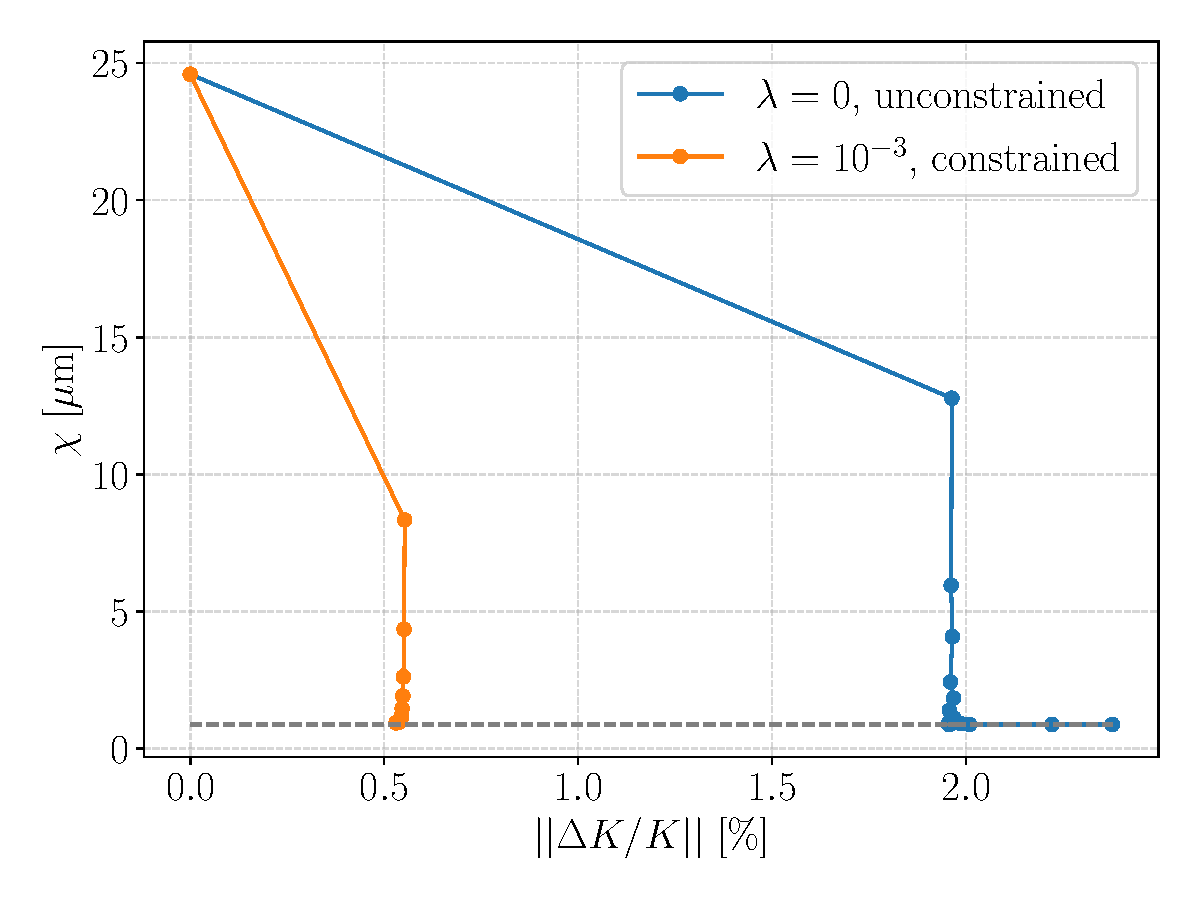
\includegraphics[width=0.75\textwidth]{figures/chi_versus_dk_cumsum.pdf}
\caption{$\chi$ versus $||\Delta K/K||$ throughout 10 LOCO iterations. The gray dashed horizontal line corresponds to $\chi = \SI{908}{\nano\meter}$, the value used as reference for convergence.}
\label{fig:chi_vs_dkl}
\end{figure}
\begin{figure}[h!]
\centering
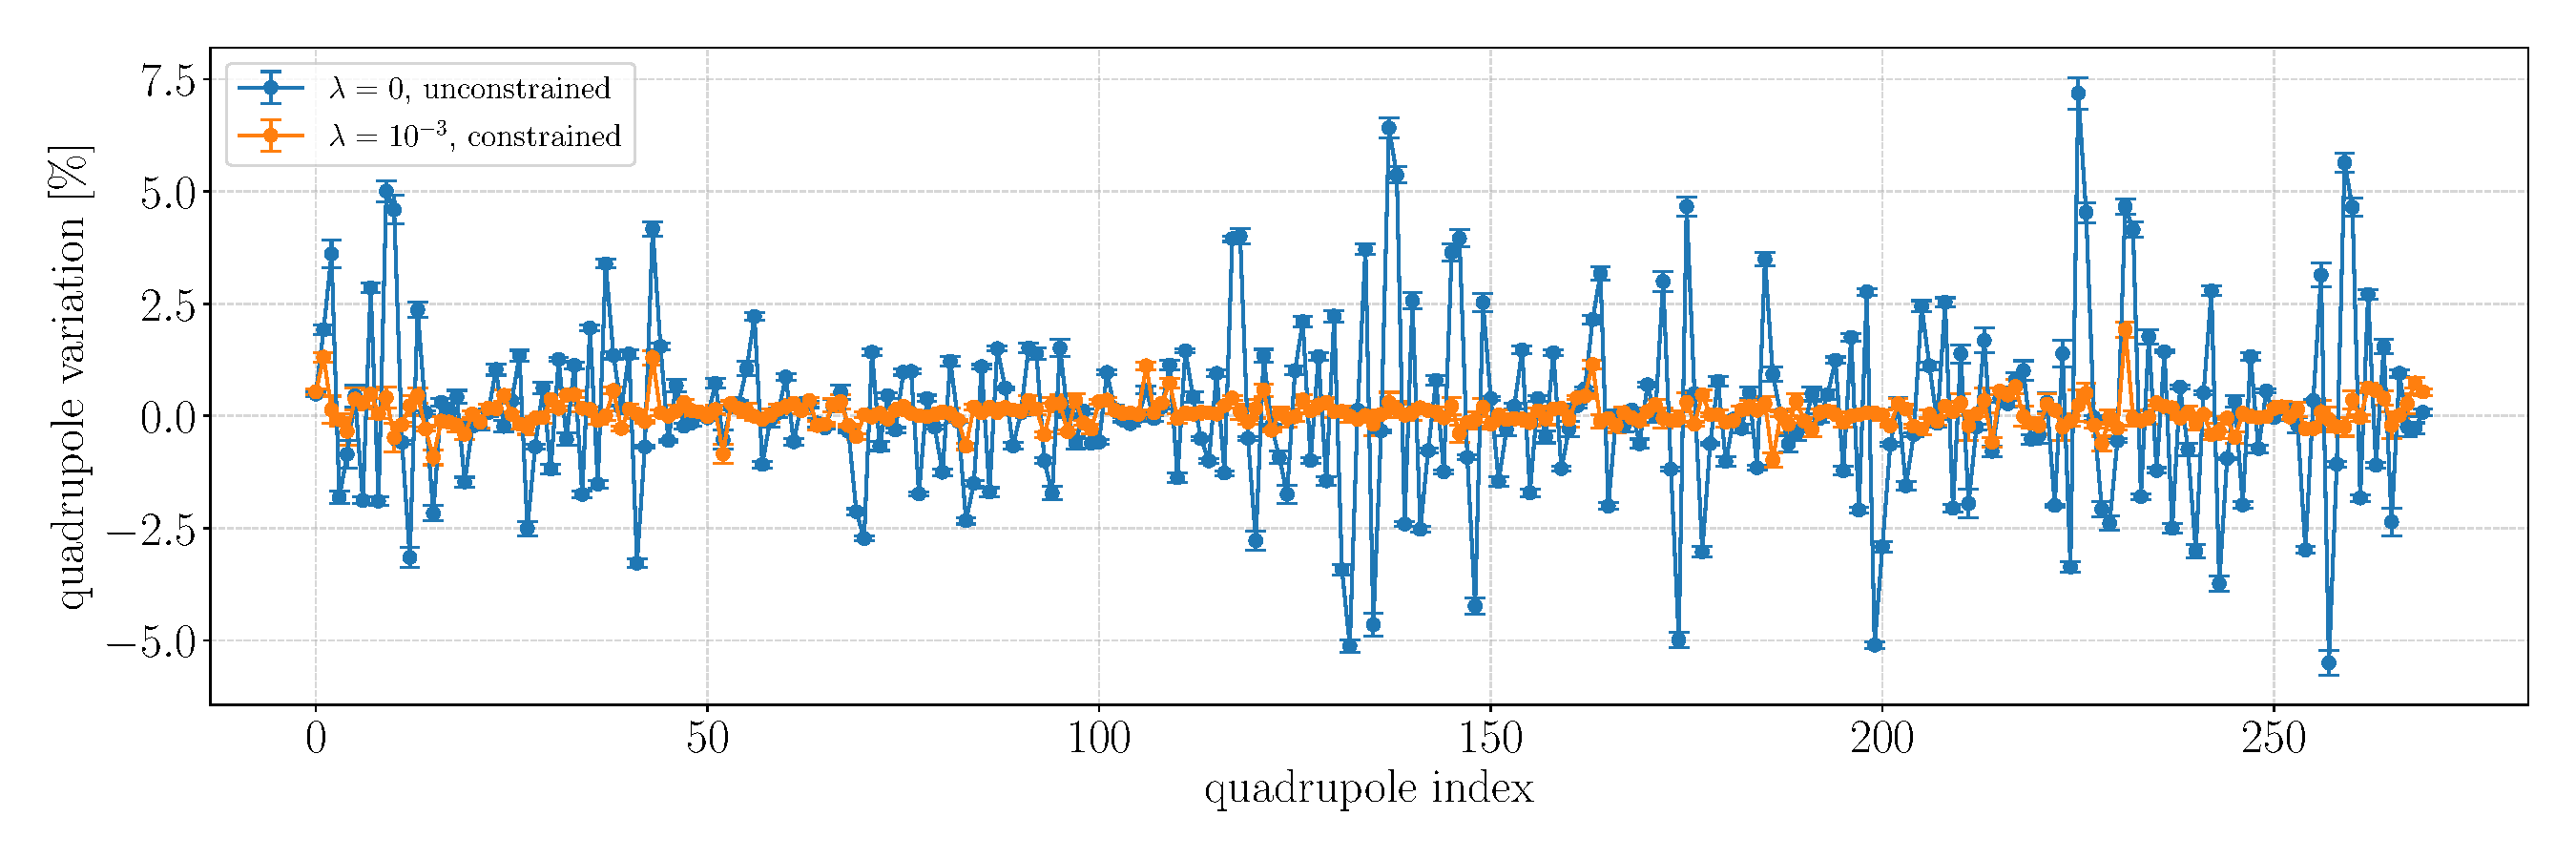
\includegraphics[width=1.0\textwidth]{figures/delta_kl_comparison_better_grid.pdf}
\caption{Comparison of quadrupoles variations obtained from LOCO with two calculation methods.}
\label{fig:dkl_compare}
\end{figure}

The variations reaching $\SI{7.5}{\%}$ are unrealistic, since previous magnetic measurements and characterizations indicate a good gradient field quality, satisfying the specification of $\SI{0.05}{\%}$ in gradient errors. Moreover, it can be seen that some adjacent quadrupoles have large variations with opposite signs, which are related to the quasi-denegeracies discussed in Section~\ref{sec:degeneracy}. The solution obtained with constraints demands much less of quadrupole variations and also adjusts the measured~\gls{orm} in the same level. The variations obtained for the other fit parameters included in the fitting agree for the two setups within the error bars, which was expected since basically the major difference is related to the constraints on quadrupoles strengths.

It is important to point out that the convergence criteria for $\chi$ should avoid the cases of over-fitting. In addition to save the LOCO running time, the most important reason is to prevent the method from increasing the quadrupoles strengths to produce a negligible reduction in $\chi$. In Figure~\ref{fig:chi_vs_dkl} it can be seen that for the unconstrained case, the last three iterations increased $||\Delta K/K||$ considerably while $\chi$ was basically the same. The over-fitting is more serious for the unconstrained case indeed, since each iteration may produce large variations on quadrupoles but it may also be a problem even for the constrained case, since accumulated small step sizes may also produce large and unnecessary variations in the final values. The convergence criteria can be controlled by defining the minimum acceptable change in the residue, given by $\chi_{\mathrm{step}}$ and the minimum level for the residue, $\chi_{\mathrm{min}}$. For the LOCO fittings performed in Sirius storage ring, the values used was $\chi_{\mathrm{step}} = \SI{10}{\nano\meter}$ and $\chi_{\mathrm{min}} = \SI{250}{\nano\meter}$, where the value for $\chi_{\mathrm{min}}$ was defined based on Sirius \glspl{bpm} accuracy. The final residue of $\SI{908}{\nano\meter}$ obtained in these fittings is still $3.6$ times greater than the \gls{bpm} accuracy and the explanation for this limit of convergence will be given throughout this chapter. Nevertheless, obtain a calibrated model with an \gls{orm} that agrees with the measured in the sub-$\mu$m level already corresponds to a very good fitting.

\subsection{Fit Parameters Variation}\label{subsec:fit_var}
As mentioned in~\cite{safranek1997}: ``\textit{the easiest way to determine how much the set of fit parameters vary due to random errors in the measurements is simply to measure many~\gls{orm}, analyze each one separately, and see how much variation there is between fit parameters for the different data sets}''. Therefore, to determine the variations of fit parameters presented in Table~\ref{tab:fit_params}, the aforementioned procedure was applied in Sirius storage ring, where 10~\glspl{orm} were measured sequentially. 

The~\gls{loco} analysis was performed in these 10 measured~\glspl{orm} with the configuration described in Subsection~\ref{subsec:loco_config} and the results are organized in Table~\ref{tab:fit_var}. The average initial residue for these 10 realizations was $\chi_{\mathrm{initial}} = \SI{9.2(4)}{\micro\meter}$ and after the convergence the average final residue was $\chi_{\mathrm{final}} = \SI{1.04(2)}{\micro\meter}$. For each fit parameter, the~\gls{std} variation obtained in the set of 10 LOCO realizations was used to define the corresponding error bars.
\begin{table}
    \centering
    \caption{Variations in fit parameters from LOCO analysis of 10 ORM measurements performed in Sirius storage ring.}
    \label{tab:fit_var}
    \begin{tabular}{cccc}
        \toprule\toprule
        Parameter & std variation & peak-to-valley variation & Unit \\
        \hline
        Quadrupole Relative Strength     & 0.13 & 0.32 & \% \\  
        H. BPM Gain             & 0.06 & 0.27 & \%\\
        H. Corrector Gain       & 0.18 & 1.03 & \%\\
        V. BPM  Gain             & 0.07 & 0.35 & \%\\
        V. Corrector Gain       & 0.21 & 1.14 & \%\\
        Skew Quadrupole Absolute Strength& \num{1.3e-4} & \num{6.2e-4} & $\SI{}{\meter^{-1}}$\\
        BPM roll angle                & 0.25 & 1.31 & $\SI{}{\milli\radian}$ \\
        \bottomrule\bottomrule
    \end{tabular}
\end{table}

For each calibrated model obtained with LOCO, the lattice functions and its variations in this set of 10 values were also calculated. The results are organized in Table~\ref{tab:twiss_var}. 
\begin{table}
    \centering
    \caption{Variations in lattice functions obtained from LOCO calibrated models from 10 ORM measurements performed in Sirius storage ring.}
    \label{tab:twiss_var}
    \begin{tabular}{cccc}
        \toprule\toprule
        Lattice function & std variation & peak-to-valley variation & Unit \\
        \hline
        $\beta_x$ & \num{0.17}& \num{0.86} & \%\\
        $\beta_y$ & \num{0.14} & \num{0.99}& \% \\
        $\eta_x$ & \num{0.26} & \num{1.36} & \SI{}{\milli\meter}\\
        $\eta_y$ & \num{0.62} & \num{2.62} & \SI{}{\milli\meter} \\
        \bottomrule\bottomrule
    \end{tabular}
\end{table}

The variations for dispersion function are calculated as absolute values because $\eta_x$ is zero in the straight sections, so it is not possible to divide the variations by the average values and then obtain a finite relative variation. To compare the variations in Table~\ref{tab:twiss_var}, the average and~\gls{std} of $\eta_x$ around the Sirius storage ring is $\SI{2.1}{\cm}$ and the peak-to-valley value is $\SI{8.3}{\cm}$. In the case of betatron functions, which always assumes positive values by definition, it is possible to obtain the relative variations.

\subsection{Initial Condition Dependence}
\gls{orm} fitting for Sirius storage ring with LOCO can be viewed as finding a minimum of a function $\chi$ with $1110$ variables (the fit parameters). The minimization problem in such high dimensions may contain multiple local minima between the starting point and the global minimum (if it exists at all). The parameters during the fitting may produce a $\chi$ that is trapped in these local minima, which might be away from more effective solutions in terms of minimizing $\chi$.

A strategy to explore the search space is beginning with different initial guesses and check the final solution obtained. If the final results are fairly independent on the initial guess, one has an indicative that, at least inside the region covered by the initial guesses range, the obtained solution is the best minimum. For a given problem, if the initial guesses cover a broad range of feasible values for fit parameters, this process indicates that, amongst the doable solutions, the found solution is the best one.

The initial condition dependence test was applied in LOCO code. An~\gls{orm} measured in Sirius storage ring was used as input for LOCO fitting. Twenty different initial conditions, regarding only the quadrupole strengths, were used to adjust the measured~\gls{orm}. The gradient initial guesses varied with a random normal distribution with $\sigma=0.5\%$ and $\sigma$ cutoff, with respect to the nominal gradients. Larger values of $\sigma$ was tested but they produced unstable dynamics in the model, thus $0.5\%$ was chosen since it allowed for the largest large of feasible initial conditions.

All the 20 initial conditions produced a greater initial $\chi$ as compared to the nominal initial guess. The minimum initial $\chi$ was $\SI{25.2}{\micro\meter}$ while with zero initial condition it was $\SI{24.6}{\micro\meter}$. Thus, the zero initial condition still was the closest to the minimum of $\chi$. The $\chi$ convergence for all the 20 realizations and the zero initial guess are plotted in Figure~\ref{fig:chi_ini_guess}. The initial $\chi$ in this test was $\SI{47(28)}{\micro\meter}$ and after 10 iterations, the final was $\SI{0.98(7)}{\micro\meter}$. Therefore, all the realizations converged to the same fitting level.
\begin{figure}[h!]
\centering
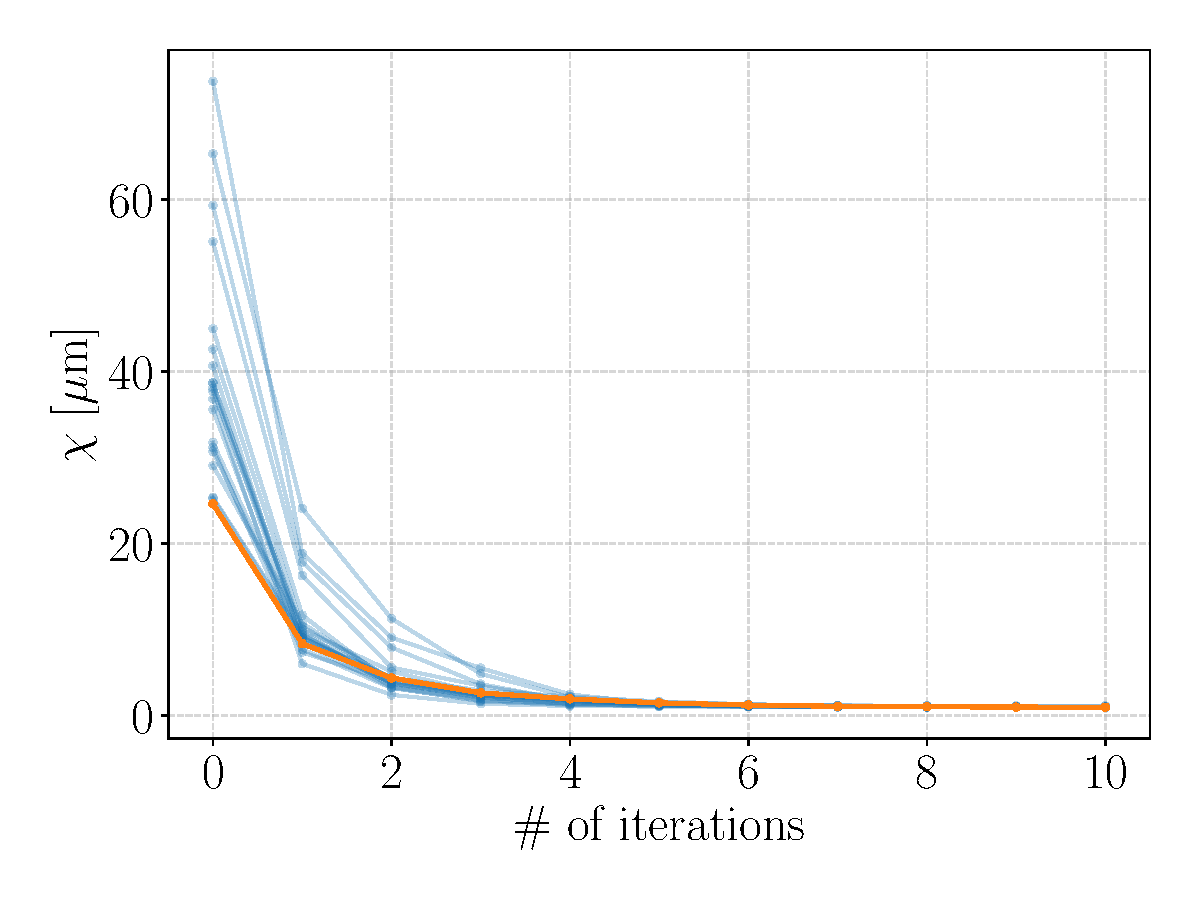
\includegraphics[width=0.75\textwidth]{figures/chi_convergence_initial_guess.pdf}
\caption{$\chi$ convergence for different initial conditions. The zero initial guess convergence is represented by the orange curve.}
\label{fig:chi_ini_guess}
\end{figure}

Figure~\ref{fig:quad_stren_ini_guess} shows the gradient solutions obtained these 20 different initial conditions and the solution obtained with zero initial guess as well. The relative variations were calculated comparing final with nominal strengths. Although the initial spread in gradients was $0.5\%$, the final spread in the fitted solutions is $0.2\%$. Moreover, the correlation between the mean of solutions and the solution obtained with zero initial guess was $98.5\%$ and the~\gls{std} difference is only $0.06\%$. For the realizations individually, the maximum and minimum correlations was $90\%$ and $71\%$, respectively.
\begin{figure}
\centering
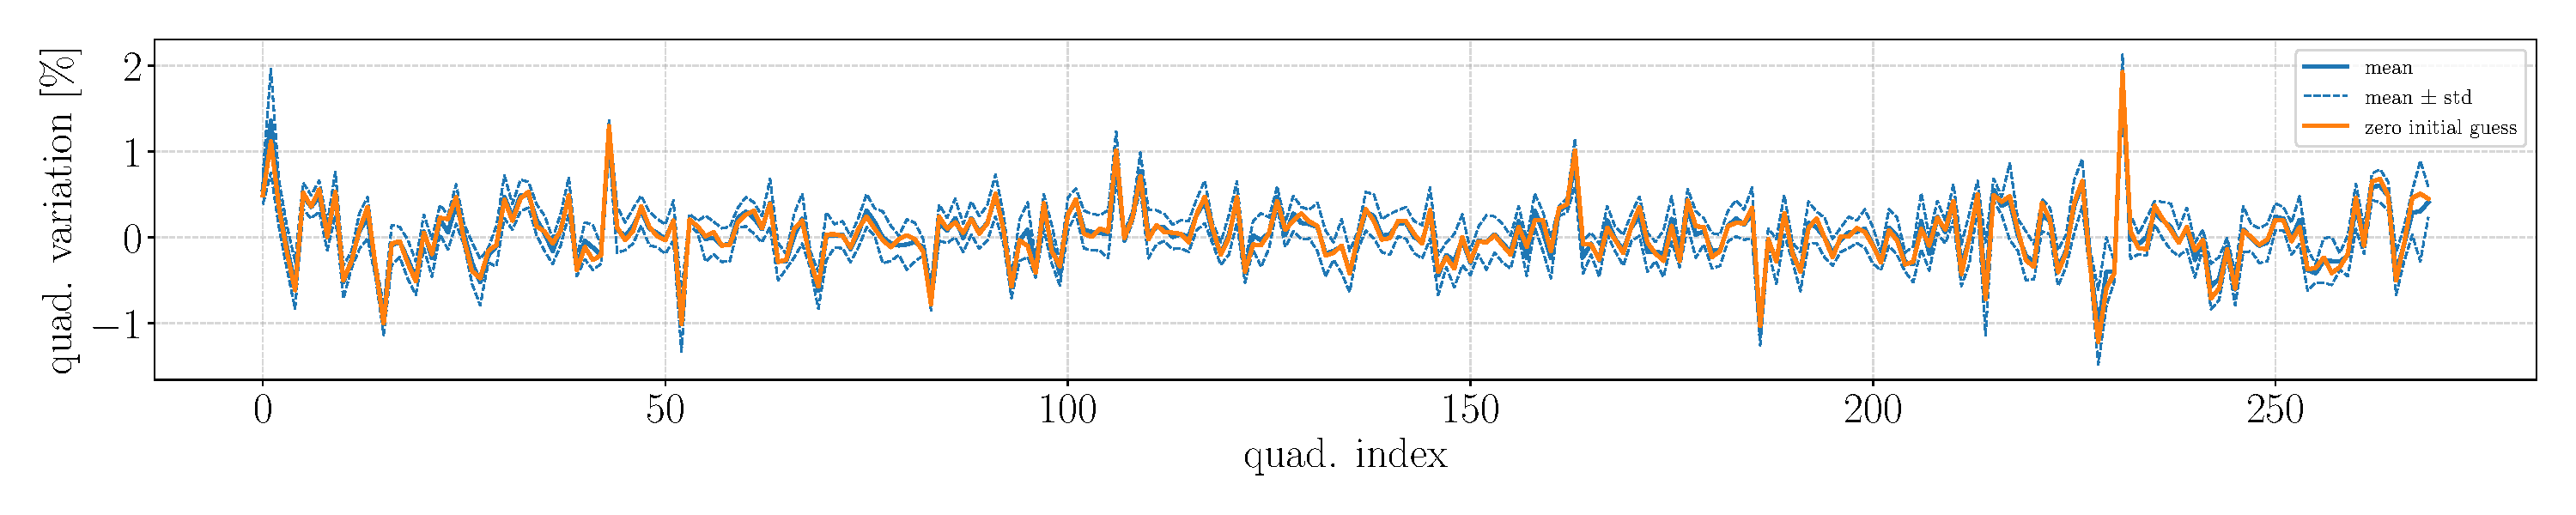
\includegraphics[width=1.0\textwidth]{figures/quad_stren_initial_guess.pdf}
\caption{Quadrupoles variations for 20 different initial guesses compared to zero initial condition.}
\label{fig:quad_stren_ini_guess}
\end{figure}

With this test one can conclude that the solution obtained with zero initial guess produces a minimum in $\chi$ that is fairly independent on the initial conditions.
\subsection{Finding Planted Error}
There is another insightful test, suggested and performed in~\cite{safranek1995}, with the goal of showing that quadrupole gradients can be accurately predicted with LOCO method. The test is quite simple: measure an~\gls{orm}, then change an individual quadrupole strength (in the case of Sirius, change the current of a trim-coil) and re-measure the~\gls{orm}. Each~\gls{orm} is adjusted with LOCO and the two sets of fitted quadrupole gradients is then compared.

The test was also performed in Sirius storage ring. The trim-coil current of a QFA quadrupole was varied to produce a $-1.19\%$ reduction in its gradient strength. This quadrupole is placed in a high-beta straight section. Following the quadrupoles sorting around the storage ring, this corresponds to the 161\ts{th} quadrupole out of 270. Figure~\ref{fig:delta_13M1_qfa} shows the test results.
\begin{figure}[h!]
\centering
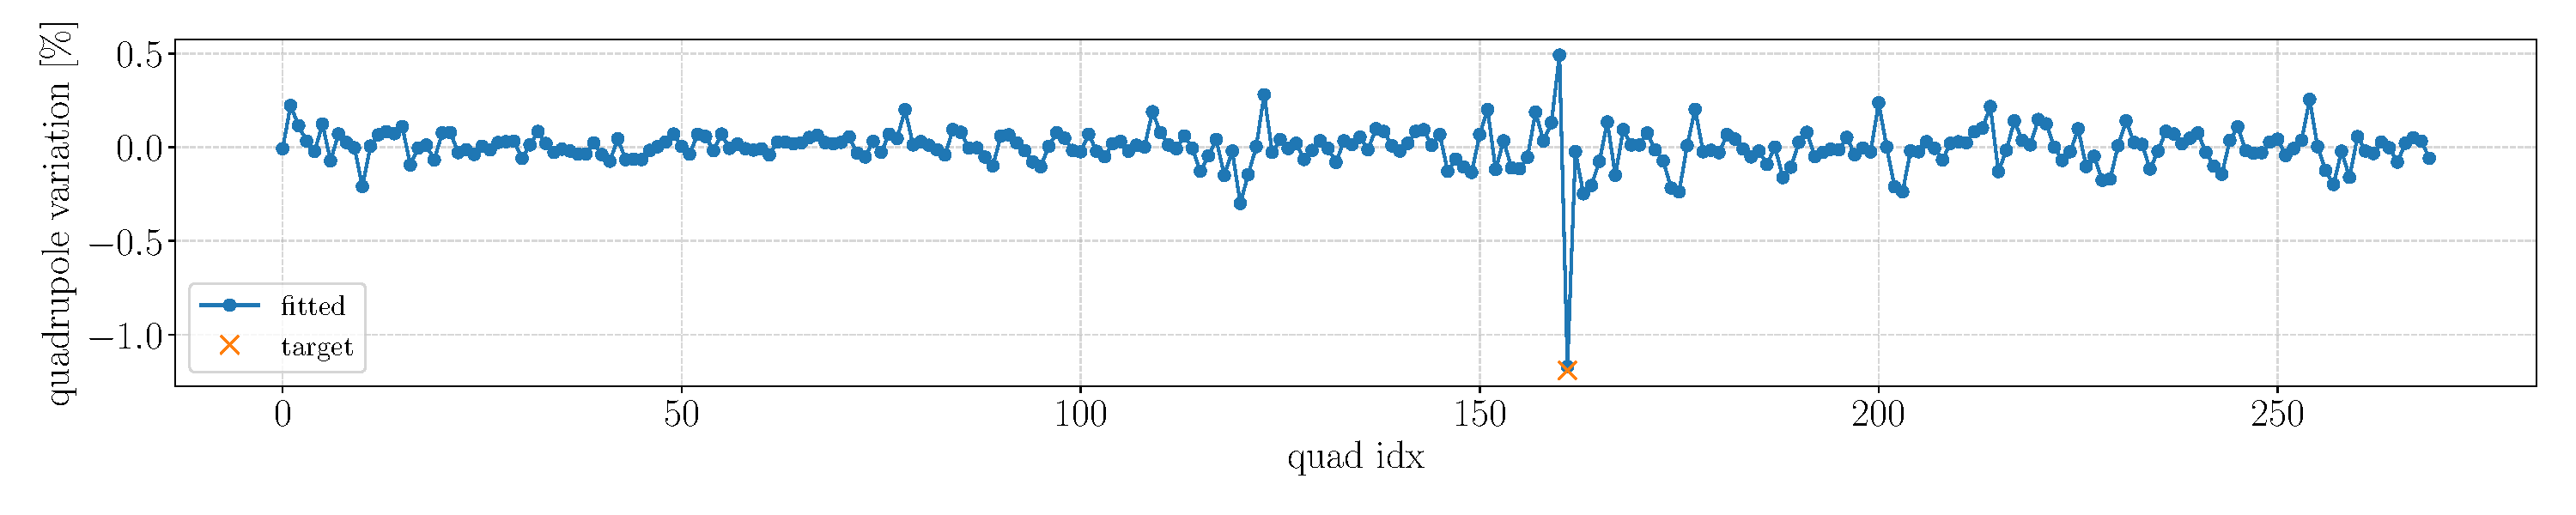
\includegraphics[width=1.0\textwidth]{figures/delta_13M1_QFA.pdf}
\caption{Quadrupoles variations comparison for two orbit response fittings, where the difference in an intentional change in the 161\ts{th} quadrupole.}
\label{fig:delta_13M1_qfa}
\end{figure}

The target gradient error in the 161\ts{th} quadrupole was $-1.19\%$. From LOCO analysis, it was found a $-1.17\%$ variation in this quadrupole. This is a disagreement between the planted and the fitted error with LOCO lesser than $2\%$. The remaining quadrupoles variations found had a $0.002\%$ average and $0.09\%$~\gls{std}. The low average indicates that these variations are related to random errors in the fit parameters and the~\gls{std} value obtained in this test is compatible with $0.13\%$, which is the std variation for quadrupoles obtained in 10 ORM measurements (Table~\ref{tab:fit_var}).

From this test, it can be concluded that LOCO analysis can accurately predict the quadrupole gradient errors in Sirius storage ring. 

\section{Orbit Response Matrix Fitting}\label{sec:orm_fit}
After an exhaustive set of tests to check the LOCO code reliability and to define the fitting setup, the method was finally applied to fit the measured~\gls{orm}, calculate the necessary corrections and download them in Sirius storage ring normal quadrupole trim-coils and skew quadrupoles as well. The process is repeated until measured and nominal~\gls{orm} coincide in a satisfactory level.

The first~\gls{orm} was measured in Sirius storage ring with a $\SI{10}{\milli\ampere}$ stored electron beam and the orbit corrected to the~\gls{bba} orbit. The operation tunes was around $\nu_x = 49.07$ and $\nu_y = 14.13$, the quadrupole trim coils and skew quadrupoles currents were all set to zero. The LOCO fitting was applied, starting from the nominal model to obtain the fit parameters presented in Table~\ref{tab:fit_params} that best explains the measured~\gls{orm}. Since the aforementioned tunes provides a better injection efficiency, it was decided that the LOCO corrections should not move the measured tunes towards the nominal values. Therefore, the nominal model used as the initial model for LOCO had its betatron tunes shifted to match measured ones, in such a way that the gradient variations obtained would be associated only to the localized errors that maintain the tunes unchanged.

Based on previous tests performed with measured data, it was observed that only including the orbit response related to~\gls{rf} frequency variation in the~\gls{orm}, i.e., including the dispersion function in the fitting, it is not sufficient make the correspondence between predicted and measured dispersion functions, both horizontal and vertical. It was necessary to include a weight factor of $2 \times 80/15 \approx 10.7$ in dispersion to reduce the fitting error. The factor $80/15$ can be understood as a normalization to compensate the difference in orbit distortions generated by a $\SI{80}{\hertz}$ variation in~\gls{rf} frequency as compared to the distortion caused by $\SI{15}{\micro\radian}$ kick change in correctors during the measurement. The factor $2$ is used to force even further the dispersion fitting. In principle, if optics distortions is caused solely by gradient errors on quadrupoles, once the measured~\gls{orm} is adjusted with the model, i.e., the beta function and phase advances in~\glspl{bpm} and correctors are fitted, the predicted dispersion function from this model should be very closed to the measured one. The need for this weight on dispersion is important and will be further discussed in Section~\ref{sec:orbit_effect}.

The initial difference between measured and nominal~\gls{orm} produced $\chi = \SI{24.6}{\micro\meter}$. After the LOCO fitting, the calibrated model produced an~\gls{orm} whose difference to the measured one was $\chi = \SI{940}{\nano\meter}$. The minimum $\chi$ obtained from LOCO fitting was almost $4$ times greater than the measured BPM accuracy. Even though the obtained $\chi$ around $\SI{1}{\micro\meter}$ represents a good level of fitting, the factor $4$ difference from the BPM accuracy values indicates that there are still some systematic errors influencing the measurements, as discussed in \cite{safranek1995}.

\subsection{Gains}
\glspl{bpm} gains, roll errors and correctors gains are parameters that are related to the correspondent devices, thus it should be independent on the machine optics and coupling. Furthermore, typically these parameters should not vary greatly, specially in such a short period of time when these measurements occurred. Therefore, it is reasonable to include the gains and roll errors as LOCO fit parameters in the first iteration and use these obtained values as initial conditions for the following fittings. It is expected that the gains will not deviate too much from the fit values obtained in the first step. From the first LOCO iteration on Sirius, the BPM gains, roll errors and correctors gains obtained are shown in Figure~\ref{fig:gain_fit}.
\begin{figure}[h!]
\centering
\begin{subfigure}[t]{0.49\textwidth}
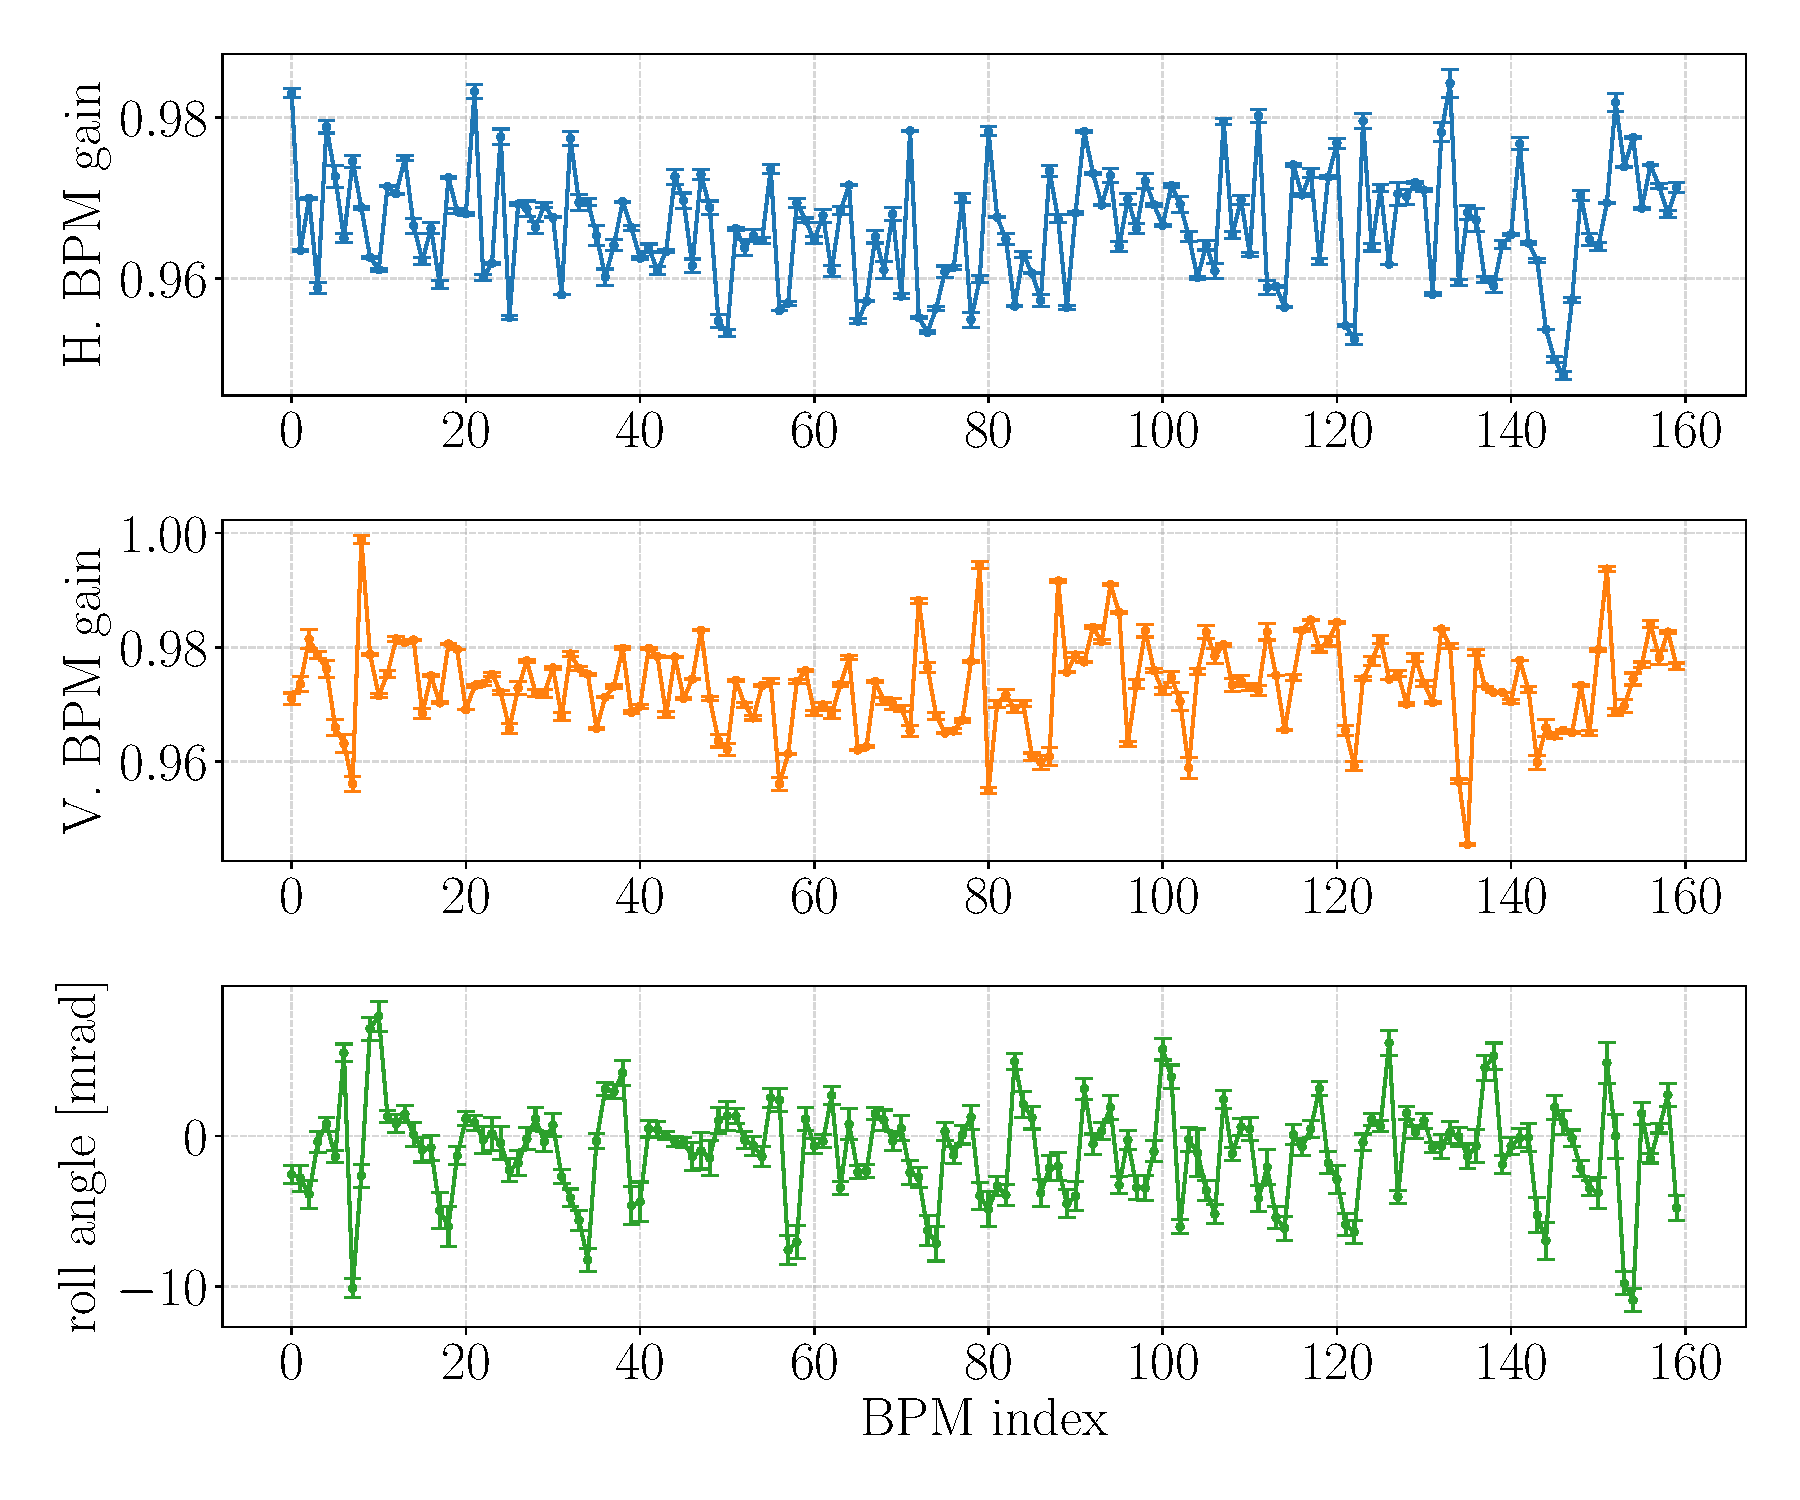
\includegraphics[width=1.0\textwidth]{figures/bpm_gains_iter0_big.pdf}
    \caption{BPM gains and roll angles.}
    \label{subfig:bpm_fit}
\end{subfigure}
 \begin{subfigure}[t]{0.49\textwidth}
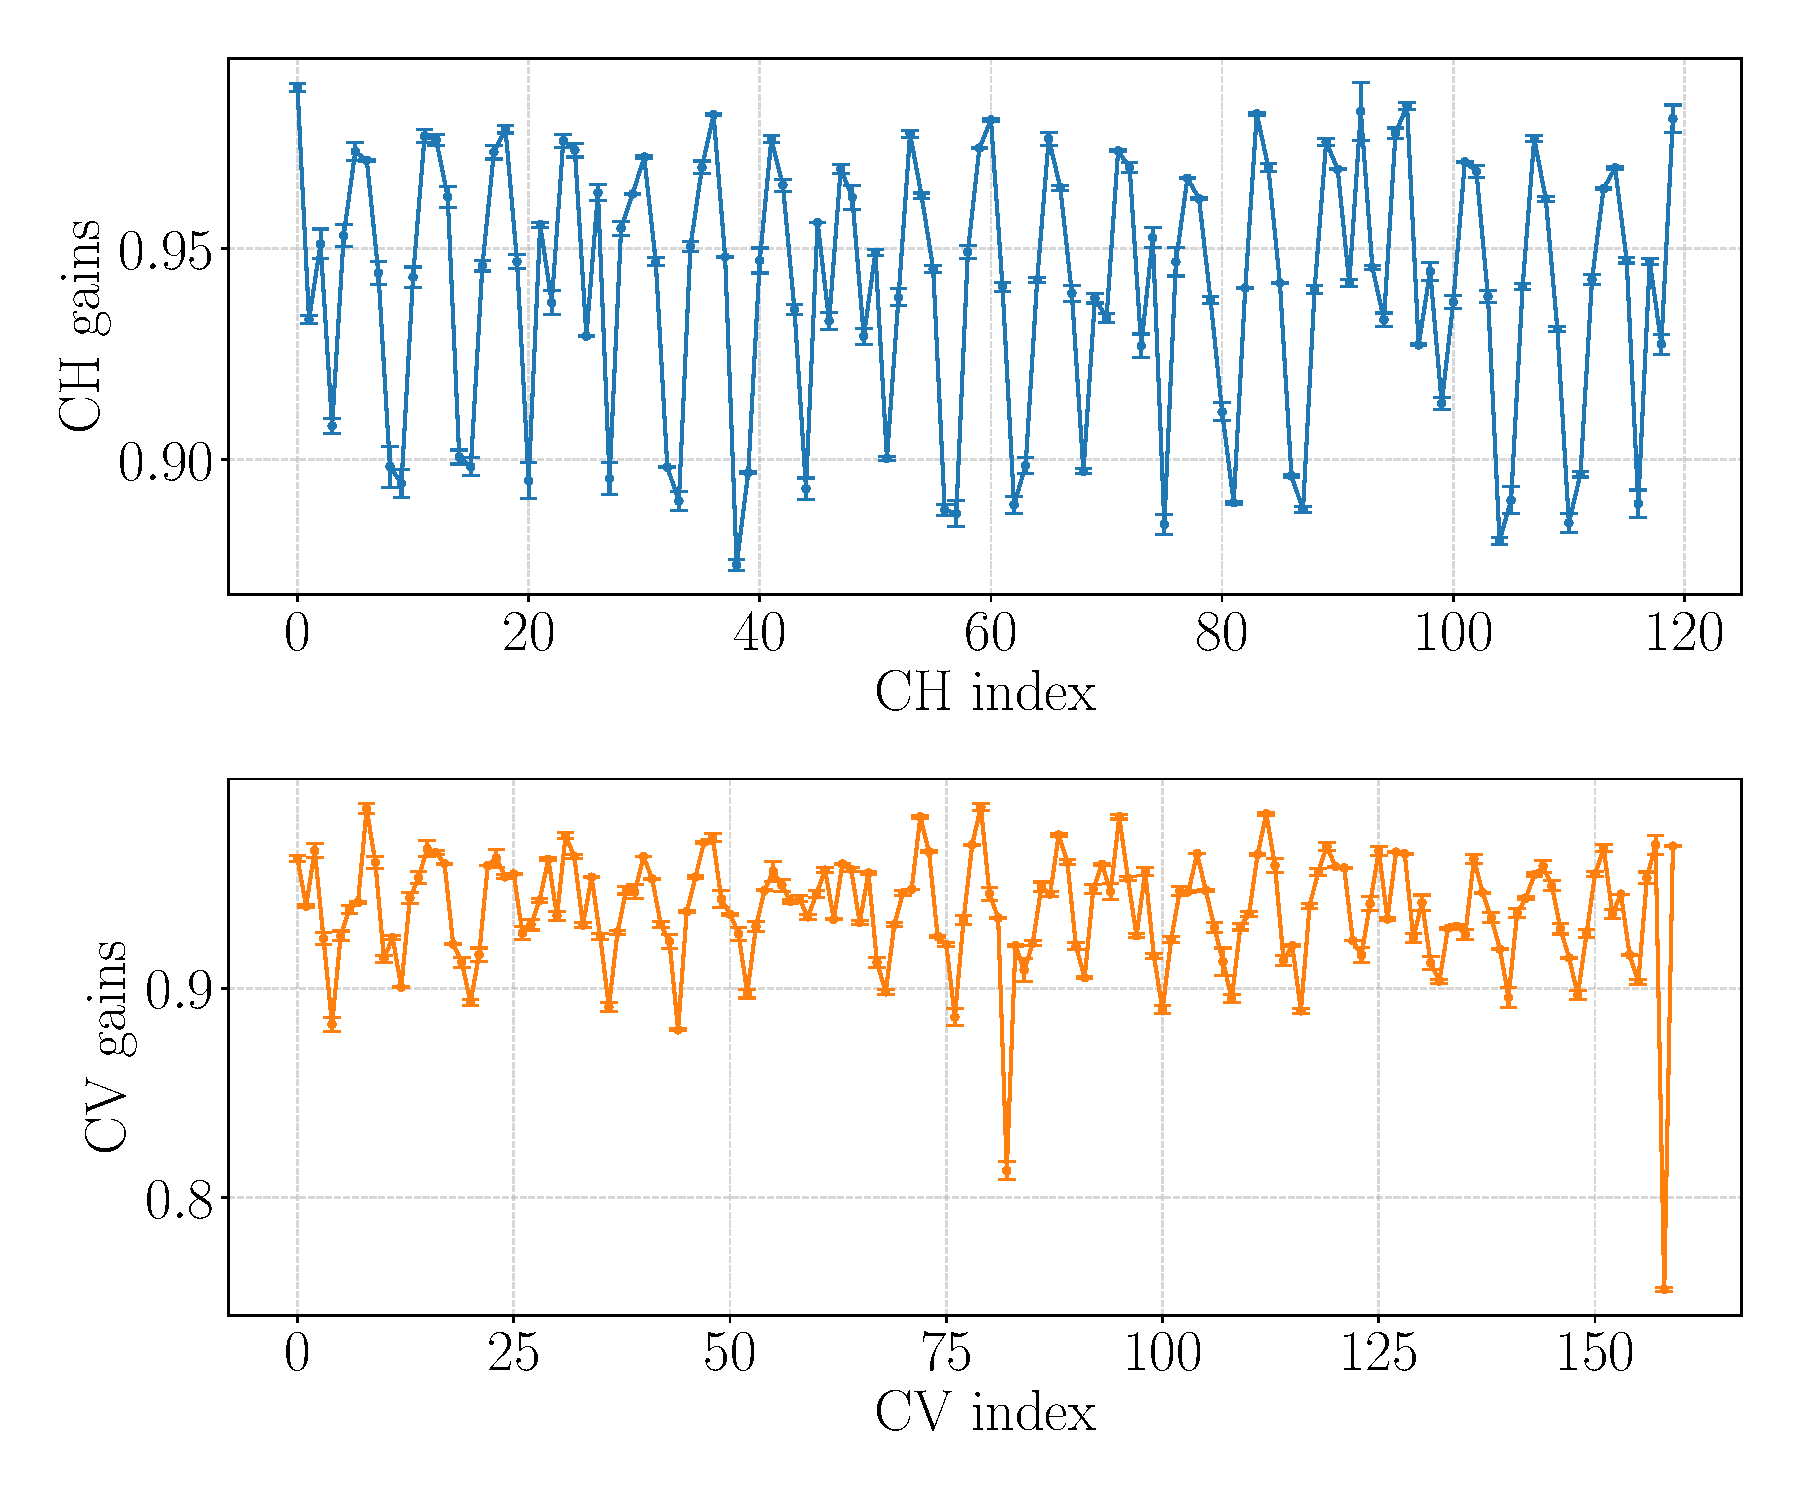
\includegraphics[width=1.0\textwidth]{figures/corr_gains_iter0_big.pdf}
    \caption{Correctors gains.}
    \label{subfig:corr_fit}
\end{subfigure}
\caption{Fitted values for BPM gains, roll errors and correctors (CH and CV) gains.}
\label{fig:gain_fit}
\end{figure}

The values in format (average $\pm$ std) for each parameter presented in Figure~\ref{fig:gain_fit} are: $\num{0.966(7)}$ for horizontal BPM gain, $\num{0.973(8)}$ for vertical BPM gain, $\num{0.94(3)}$ for CH gain, $\num{0.94(4)}$ for CV gain and $\SI{-1(3)}{\milli\radian}$ for BPM roll error. As discussed in Appendix~\ref{appendix:gains}, the interpretations for BPM and correctors gains are opposite, in the sense that for BPMs the fitted gains represents the corrections factors that should be applied in the measurements to explain correctly the actual orbit distortions, while it is the inverse of correctors gains that should be used in the kick applied to obtain the actual kicks that affected the beam. Therefore, this fitting indicates that the actual BPMs measurements are around $3\%$ lower than the actual values, on average, and the actual kicks that distort the beam orbit are $6\%$ greater (on average) than the kicks variations ($\SI{15}{\micro\radian}$) considered by the control system during~\gls{orm} measurement. It also can be observed that the spread between BPM gains is one order of magnitude lower than the spread between correctors and this difference was already expected.

In Figure~\ref{subfig:corr_fit} it can be observed a 20-fold periodic pattern in correctors gains, specially in CH gains. This signature following the storage ring period is also correlated to the topic of Section~\ref{sec:orbit_effect}. It also can be seen two outliers in CV gains in 82\ts{th} and 158\ts{th} vertical correctors. These correctors were later examined on site but this initial survey did not reveal any anomalies. The cause for these outliers in CV gains is still under investigation and they did not compromise the following results.

As already mentioned, the fitted gains obtained from the first LOCO iteration and presented in Figure~\ref{fig:gain_fit} were used as initial values for the following iterations. For this study, the obtained values were not used in the control system to correct the BPM measurements nor the correctors excitation curves. This was decided since the fitted gains are close to unity and they do not compromise greatly the orbit correction system and the~\gls{orm} measurement. For machine studies in the future, when much finer tuning in storage ring and control system will be performed, the fitted gains and roll errors may also be included as correction factors for BPMs and correctors.

\subsection{Quadrupoles Gradients}
Normal and skew gradients were also included as LOCO fit parameters to adjust the measured~\gls{orm}. The normal gradients are associated to the corrections that can be applied in 270 quadrupoles trim-coils in Sirius storage ring and skew gradients to the 80 skew quadrupoles coils installed inside some sextupoles.

The LOCO fitting changes the model parameters to calibrated it with the real machine, so the integrated gradients are changed by $\mathrm{KL}_{\mathrm{nominal}} \rightarrow \mathrm{KL}_{\mathrm{nominal}} + \Delta\mathrm{KL}_{\mathrm{LOCO}}$. The same is valid for $\mathrm{KsL}$, the skew gradients strength, however the difference is that initially the skew gradients are zero, since in the nominal model the coupling is zero as well. Ideally, $\mathrm{KL}_{\mathrm{actual}} = \mathrm{KL}_{\mathrm{nominal}} + \Delta\mathrm{KL}_{\mathrm{LOCO}}$ represents the actual focusing strengths affecting the electron beam in the real storage ring. In the real machine it is wanted to reverse this process, moving the focusing strengths towards the nominal values. Therefore, the gradient variations calculated from LOCO was applied to the machine with the opposite sign, making $\mathrm{KL}_{\mathrm{actual}} - \Delta\mathrm{KL}_{\mathrm{LOCO}} \rightarrow \mathrm{KL}_{\mathrm{nominal}}$. For skew quadrupoles, it is expected that the applied corrections cancels out the unwanted skew gradients in the storage ring to result in $\mathrm{KsL} = 0$, which is the nominal.

The process of measuring an~\gls{orm}, fitting it with LOCO and applying the corrections to the machine was realized only twice until the convergence was reached. The corrections distribution history both for normal quadrupoles and skew quadrupoles are shown in Figure~\ref{fig:loco_corrections}. The standard deviations of these corrections for each LOCO iteration are organized in Table~\ref{tab:corr_converge}.
\begin{figure}[h!]
\centering
\begin{subfigure}[t]{1.0\textwidth}
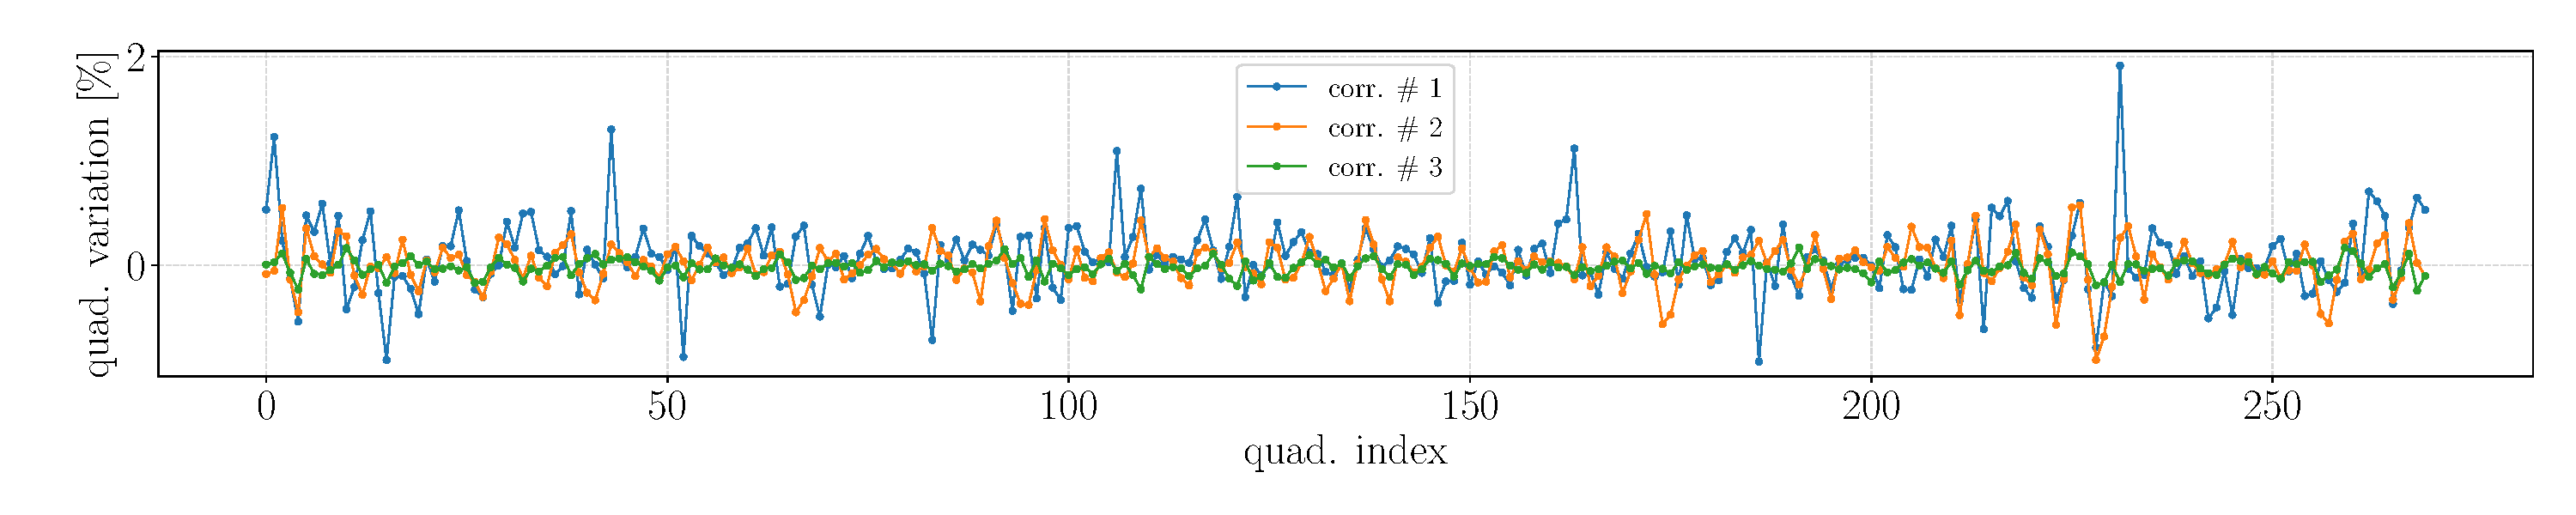
\includegraphics[width=1.0\textwidth]{figures/loco_quad_big.pdf}
    \caption{Quadrupoles trim-coils.}
    \label{subfig:quad_fit}
\end{subfigure}
 \begin{subfigure}[t]{1.0\textwidth}
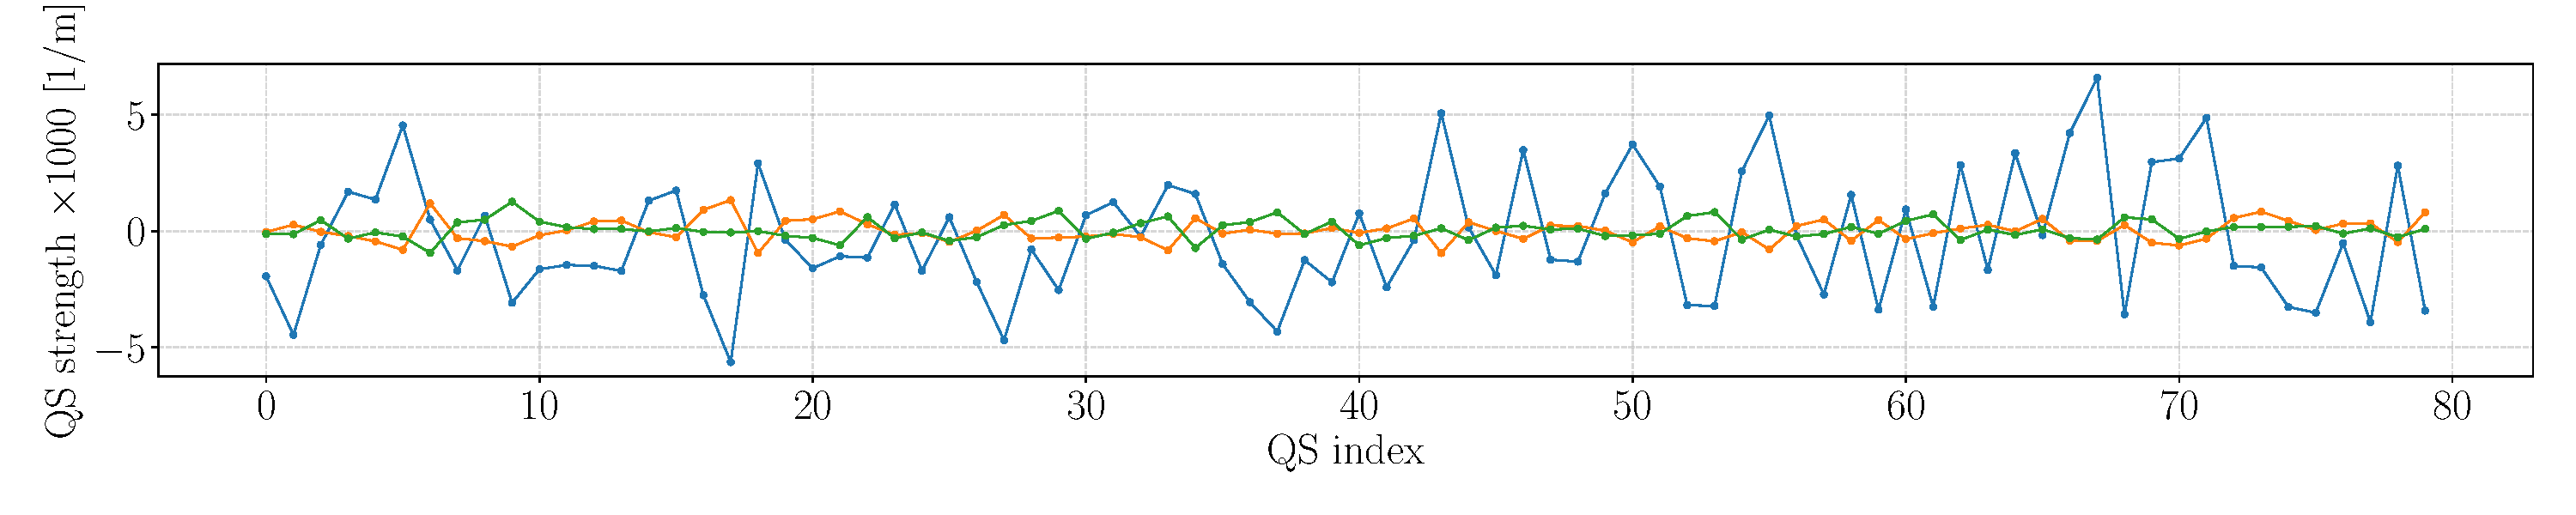
\includegraphics[width=1.0\textwidth]{figures/loco_qs_big.pdf}
    \caption{Skew quadrupoles.}
    \label{subfig:qs_fit}
\end{subfigure}
\caption{Normal and skew quadrupoles strength variations throughout LOCO iterations.}
\label{fig:loco_corrections}
\end{figure}
\begin{table}[h!]
    \centering
    \caption{Corrections strengths variation for each LOCO iteration.}
    \label{tab:corr_converge}
    \begin{tabular}{ccccc}
        \toprule\toprule
        Knobs variation (std) & corr. \#1 & corr. \#2 & corr. \#3 & Unit \\
        \hline
        Quadrupoles & \num{0.33} & \num{0.21} & \num{0.07} &\SI{}{\%}\\
        Skew Quadrupoles & \num{2.7e-3} & \num{5e-4} & \num{4e-4} & \SI{}{\meter^{-1}} \\
        \bottomrule\bottomrule
    \end{tabular}
\end{table}

From Figure~\ref{fig:loco_corrections} and the values in Table~\ref{tab:corr_converge} it can be seen that the corrections calculated in third LOCO iteration and the respective parameters variations obtained, presented in Table~\ref{tab:fit_var}, are commensurable. Therefore, it did not make sense to apply this third set of corrections, since its values already reached the limit given by the method precision so it was considered at this stage that the corrections converged. This is why only two LOCO corrections were applied in Sirius storage ring.
% \begin{figure}
% \centering
% \begin{subfigure}[t]{0.49\textwidth}
% 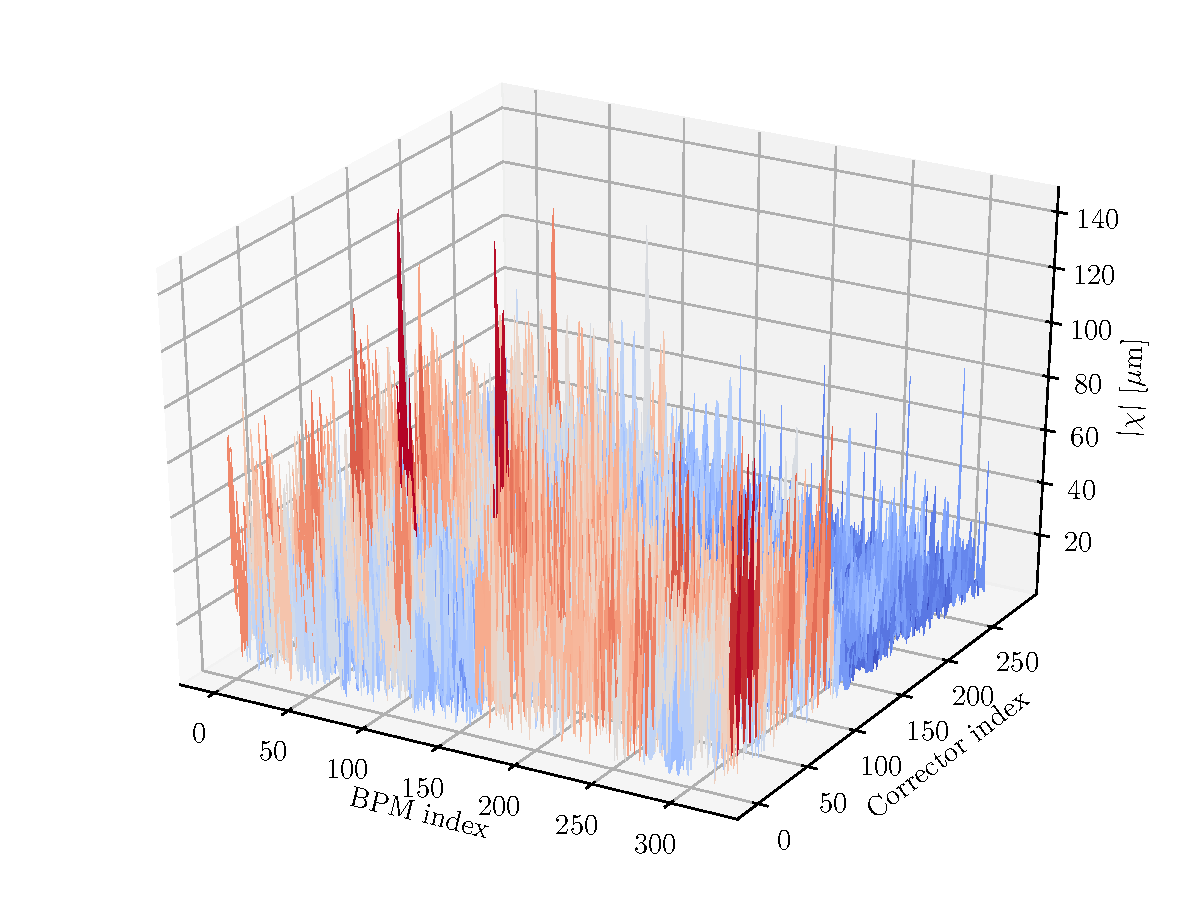
\includegraphics[width=1.0\textwidth]{figures/surface_before_loco.pdf}
%     \caption{Before.}
%     \label{subfig:ondiag}
% \end{subfigure}
%  \begin{subfigure}[t]{0.49\textwidth}
% 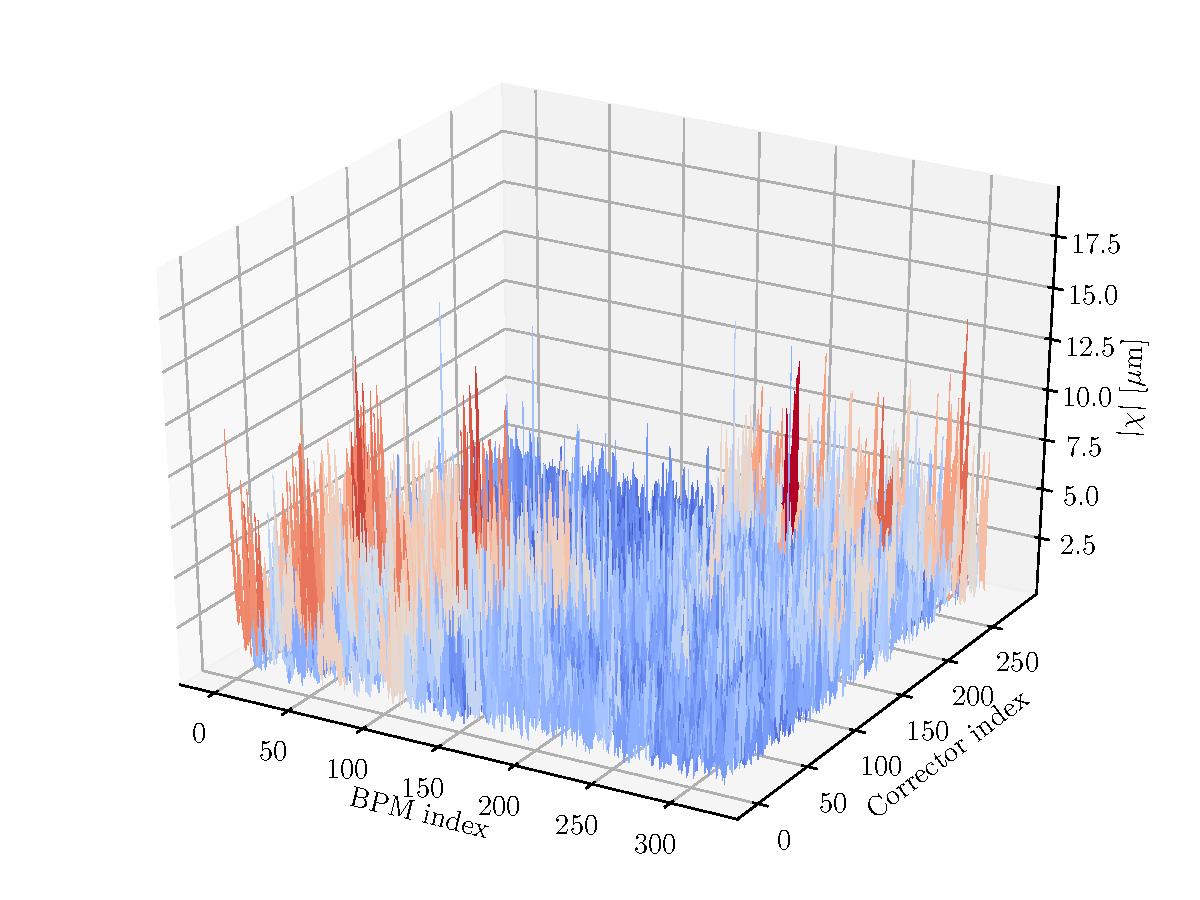
\includegraphics[width=1.0\textwidth]{figures/surface_after_loco.pdf}
%     \caption{After.}
%     \label{subfig:offdiag}
% \end{subfigure}
% \caption{Orbit response matrix error surface before and after LOCO corrections.}
% \label{fig:hist}
% \end{figure}

\subsection{Deviations from Nominal}
The figure of merit to be minimized with LOCO method is the difference between measured and calculated~\gls{orm} in each iteration, by changing the storage ring model. As LOCO corrections are applied to the machine, it is expected that the measured~\gls{orm} converges to the nominal~\gls{orm}. Table~\ref{tab:orm_progress} shows the progress of~\gls{orm} differences (represented by $\chi$) throughout LOCO corrections applied to the machine and also the fitting level for each particular iteration.
\begin{table}[h!]
    \centering
    \caption{ORM fitting progress.}
    \label{tab:orm_progress}
    \begin{tabular}{ccc}
        \toprule\toprule
        LOCO iteration & Initial $\chi$ [$\SI{}{\micro\meter}$] & Final $\chi$ [$\SI{}{\nano\meter}$] \\
        \hline
        \#1 & 24.6 & 940 \\
        \#2 & 2.7 & 895 \\
        \#3 & 2.1 & 921 \\
        \bottomrule\bottomrule
    \end{tabular}
\end{table}

The LOCO corrections applied in Sirius storage ring decreased the difference between measured and nominal~\gls{orm} from $\SI{24.6}{\micro\meter}$ to $\SI{2.1}{\micro\meter}$, which is almost a factor $12$ of reduction.

For a global view of measured~\gls{orm} convergence towards the nominal, Figure~\ref{fig:histogram} shows the histogram of errors for each LOCO iteration. The error histograms are divided in four parts, following the four~\gls{orm} blocks: $M_{xx}$, $M_{yy}$ (on-diagonal) and $M_{xy}$, $M_{yx}$ (off-diagonal). 
\begin{figure}[h!]
\centering
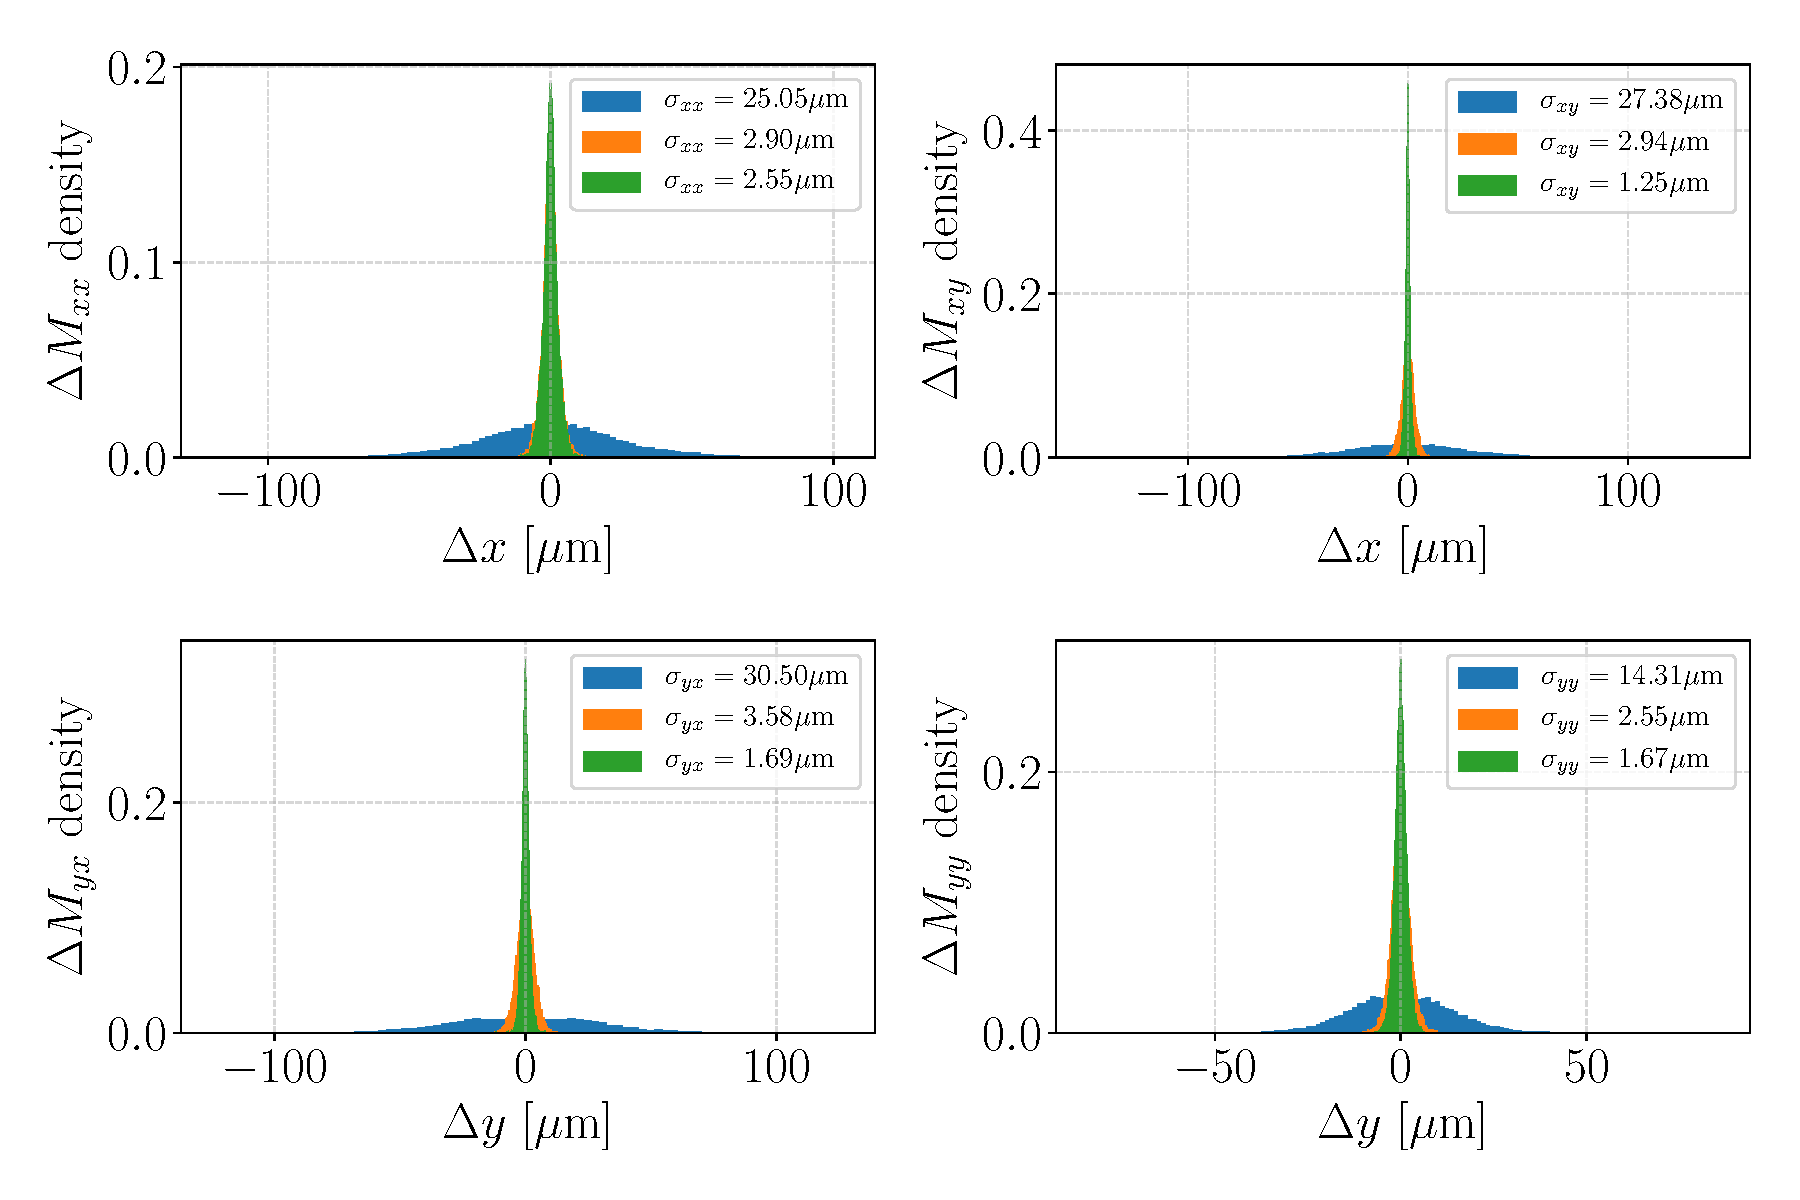
\includegraphics[width=1.0\textwidth]{figures/histogram_loco_iterations3_density.pdf}
\caption{Histogram for the errors between measured and nominal orbit response matrices for each LOCO iteration. The blue data refers to the measured ORM without corrections applied. The orange data was obtained after the first application of LOCO corrections. The green data is related to the second and last LOCO round applied.}
\label{fig:histogram}
\end{figure}

It can be seen that initially the order of magnitude of errors are basically the same for all blocks. The off-diagonal errors (related to coupling errors) are slightly greater than the on-diagonal errors. After the first correction application in the storage ring, the errors in the four blocks were already greatly reduced. After the second and final corrections the~\gls{std} errors were reduced by the following factors: 
\begin{align*}
    \sigma_{xx}^{\mathrm{initial}}/\sigma_{xx}^{\mathrm{final}} = 9.8, & \hspace{1.5cm} \sigma_{xy}^{\mathrm{initial}}/\sigma_{xy}^{\mathrm{final}} = 21.9, \\
    \sigma_{yx}^{\mathrm{initial}}/\sigma_{yx}^{\mathrm{final}} = 18.0, & \hspace{1.5cm}
    \sigma_{yy}^{\mathrm{initial}}/\sigma_{yy}^{\mathrm{final}} = 8.6. 
\end{align*}

The off-diagonal errors were reduced by a factor of 2 greater than the on-diagonal errors.

Two~\gls{orm} columns were taken to exemplify typical differences between measured and nominal matrices, before and after LOCO corrections and the results are presented in Figure~\ref{fig:orm_rows}. The first column is related to a horizontal corrector signature and the second one to a vertical corrector. Multiplying the~\gls{orm} column by the kicks $\Delta\theta_x$ and $\Delta\theta_y$, one can obtain the orbit distortion signature $\Delta x$ and $\Delta y$.
\begin{figure}[h!]
\centering
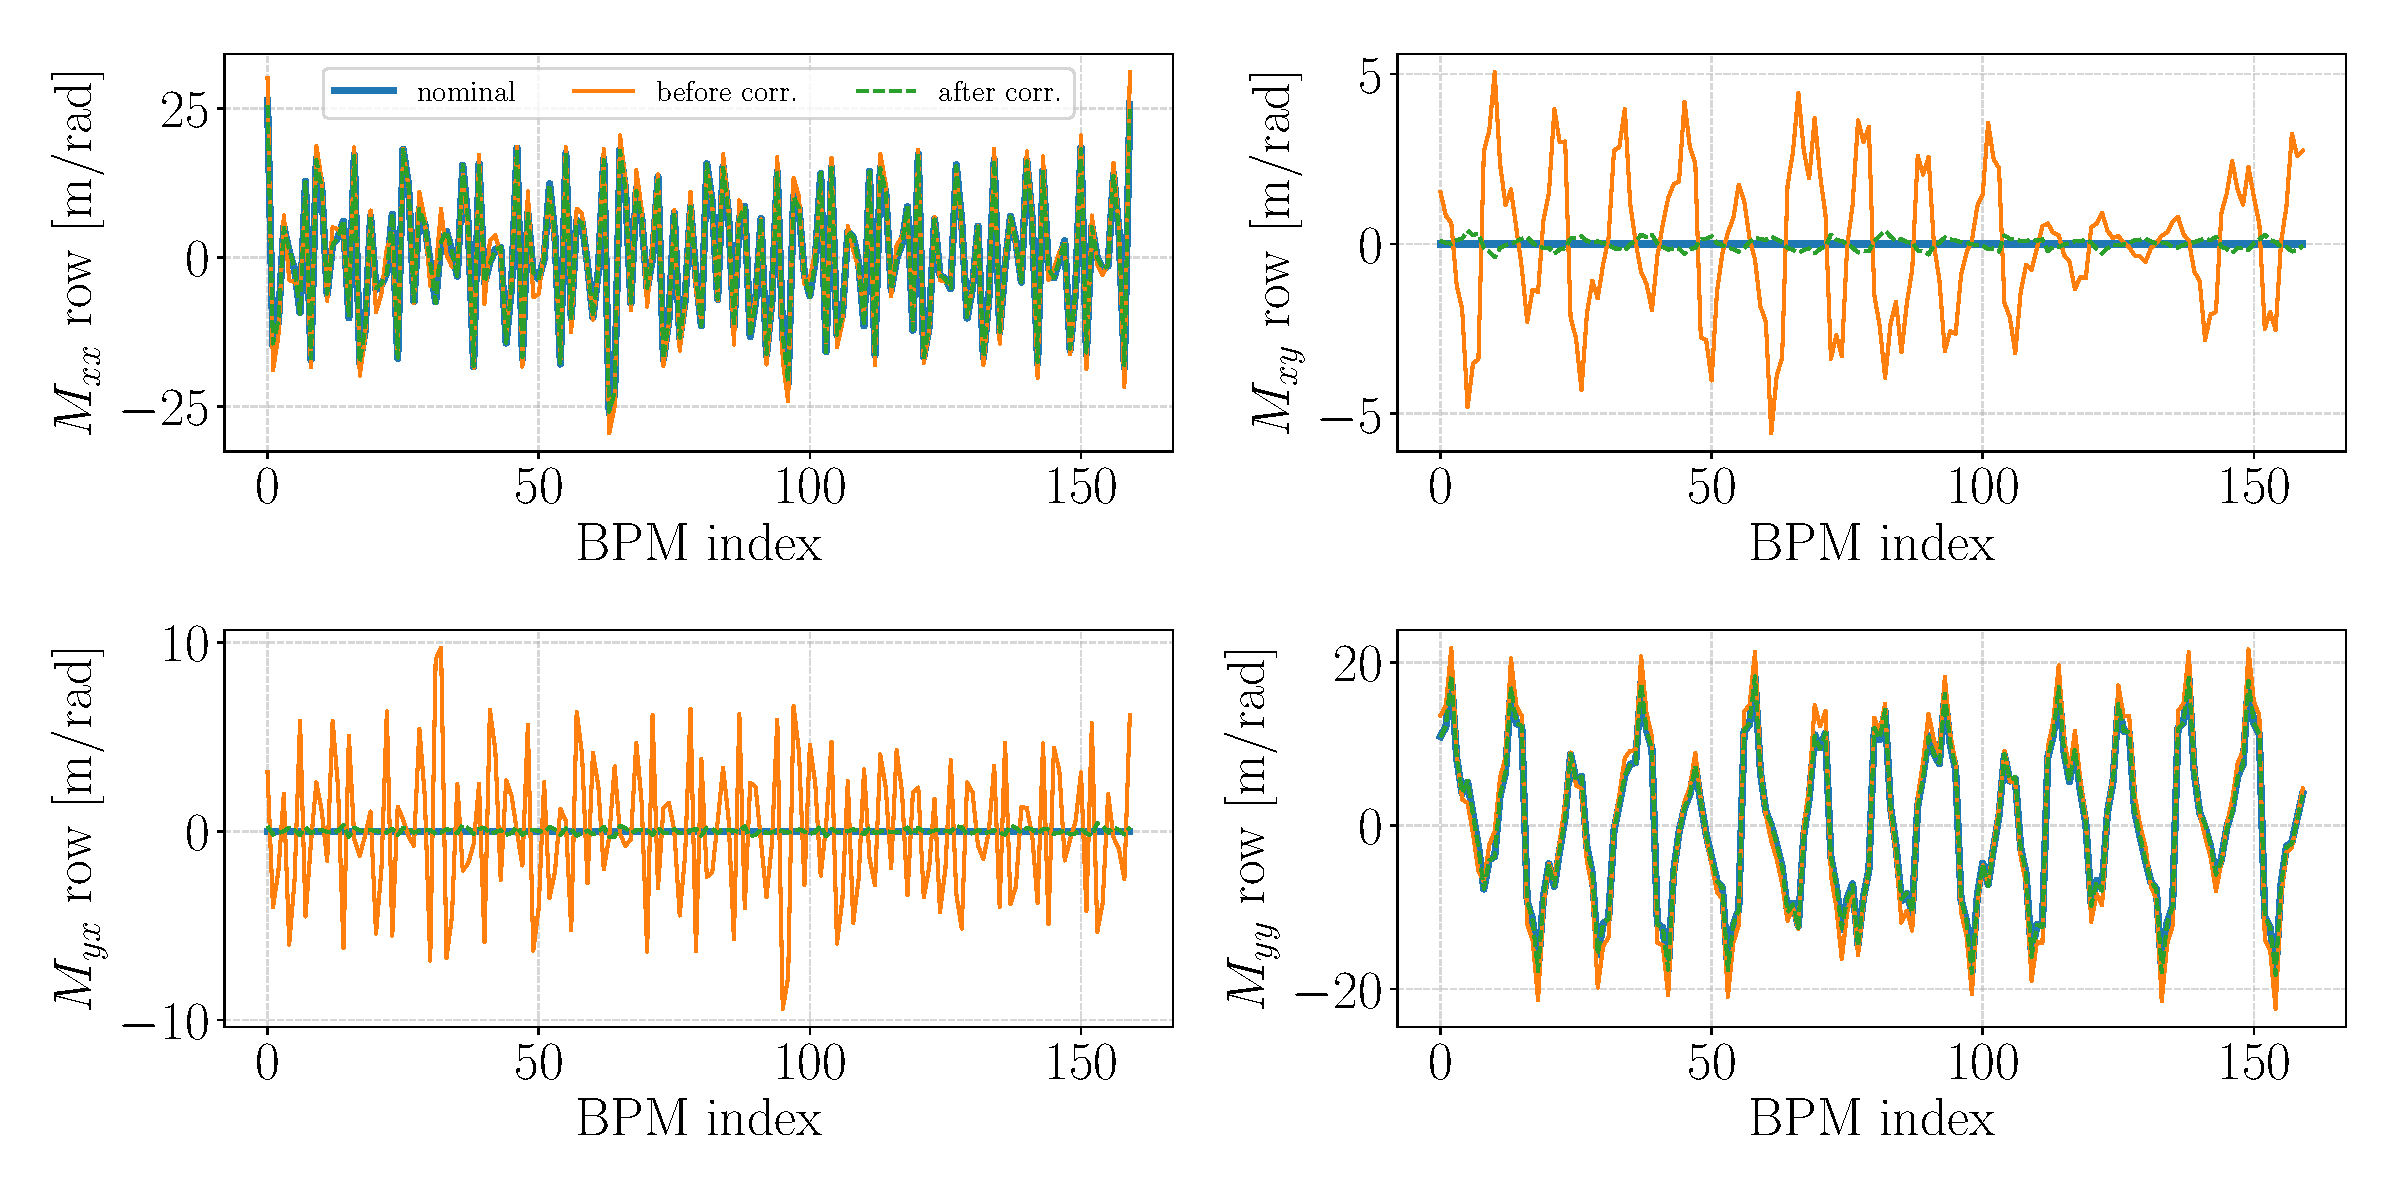
\includegraphics[width=1.0\textwidth]{figures/nominal_measured_after_before_loco_big.pdf}
\caption{Orbit Response Matrix rows for the first CH and CV. The blue curve is the nominal ORM, the orange curve represents the measured ORM before LOCO corrections and the green curve is from measured ORM after LOCO.}
\label{fig:orm_rows}
\end{figure}

In this example it can be seen that the off-diagonal elements are greatly reduced and are close to zero after corrections. The on-diagonal elements for measured and nominal~\gls{orm} are practically overlapped.

\subsection{Final Corrections}
Adding up the corrections sets for normal and skew quadruploles gradients in the two LOCO iterations, the final corrections are obtained and plotted in Figure~\ref{fig:loco_corrections_final}.
\begin{figure}
\centering
\begin{subfigure}[t]{1.0\textwidth}
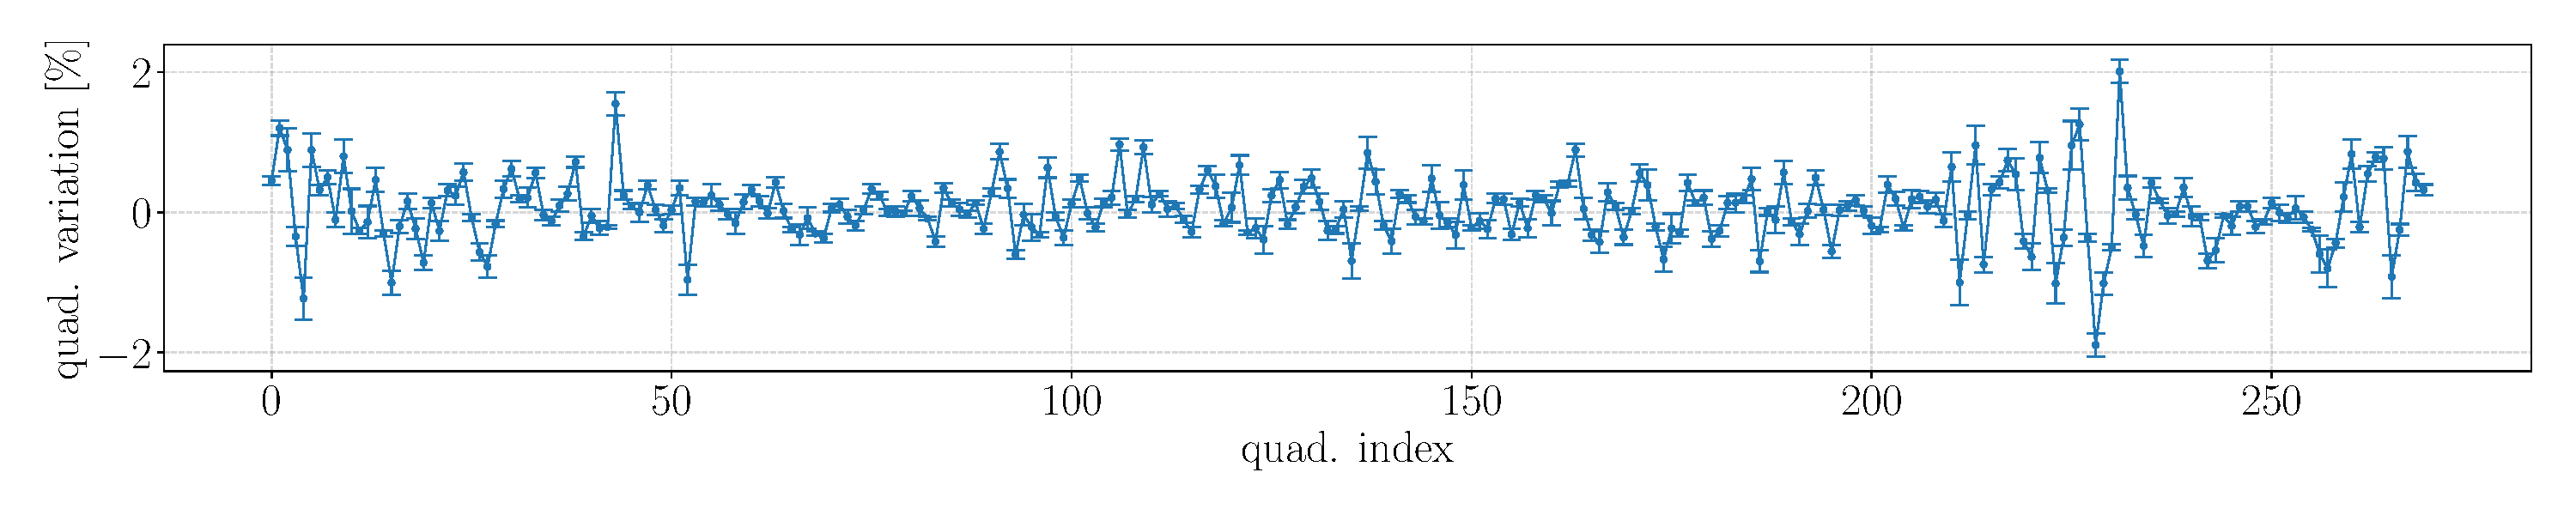
\includegraphics[width=1.0\textwidth]{figures/loco_quad_corrections_errorbar_big.pdf}
    \caption{Quadrupoles trim-coils.}
    \label{subfig:quad_fit_final}
\end{subfigure}
 \begin{subfigure}[t]{1.0\textwidth}
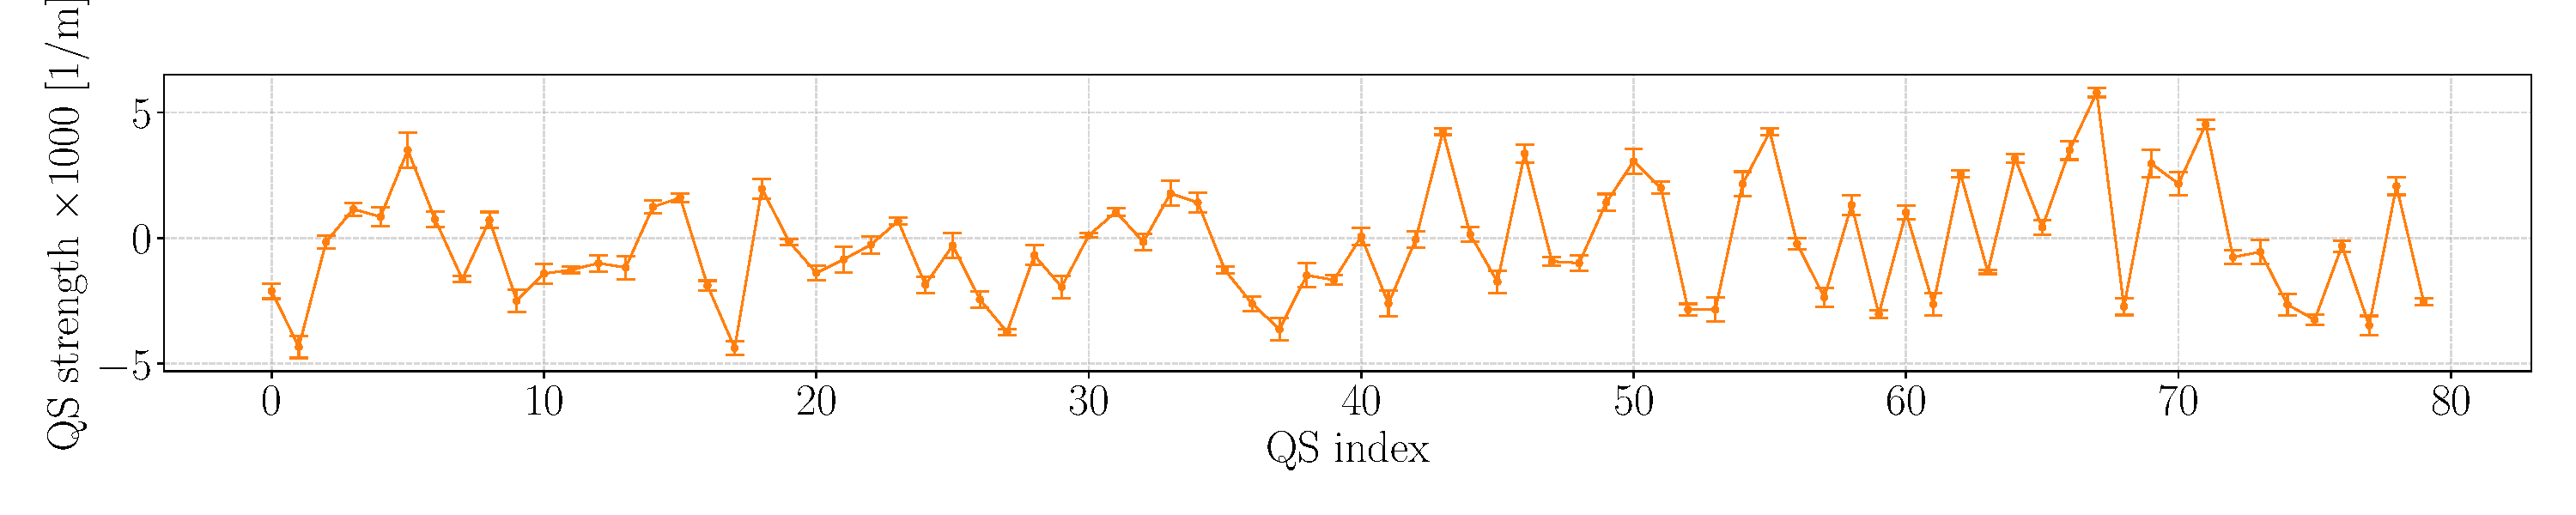
\includegraphics[width=1.0\textwidth]{figures/loco_qs_corrections_errorbar_big.pdf}
    \caption{Skew quadrupoles.}
    \label{subfig:qs_fit_final}
\end{subfigure}
\caption{Normal and skew quadrupoles final corrections.}
\label{fig:loco_corrections_final}
\end{figure}

The final quadrupole gradients variations covers the range of $\pm 2\%$, while the skew quadrupole strengths are between $\pm \SI{5e-3}{\meter^{-1}}$. Based only on magnetic characterization of quadrupoles fields, variations of $2\%$ are large, since the specifications for gradient errors were $0.05\%$. On the other hand, it is important to remember that these quadrupole variations are corrections for gradient errors along the whole storage ring. Thus, it is more likely that these corrections are compensating other sources of gradient errors. The most important ones are: additional gradients in dipoles that are not considered in the magnet modelling; gradients in sextupoles, which may be caused by additional fields in the magnets and by feed-down effect (Appendix~\ref{appendix:feed-down} for details) from misalignment or orbit distortions in sextupoles; gradient fields introduced by the undulators installed in storage ring. These other sources of gradient errors may accumulate in such a way that quadrupole variations on the order of $2\%$ are necessary for compensation.

An interesting way to visualize the quadrupole variations is dividing them by following the 12 quadrupoles families in storage ring. The magnets that make up each family were selected in order to minimize the spread in gradient strengths within the families and to satisfy the $0.05\%$ specification on gradient errors. The results of this rearrangement in families are shown in Figure~\ref{fig:loco_corrections_final_families}. The statistics for these quadrupole variations divided by families are organized in Table~\ref{tab:quad_fam_corr}.
\begin{figure}[h!]
\centering
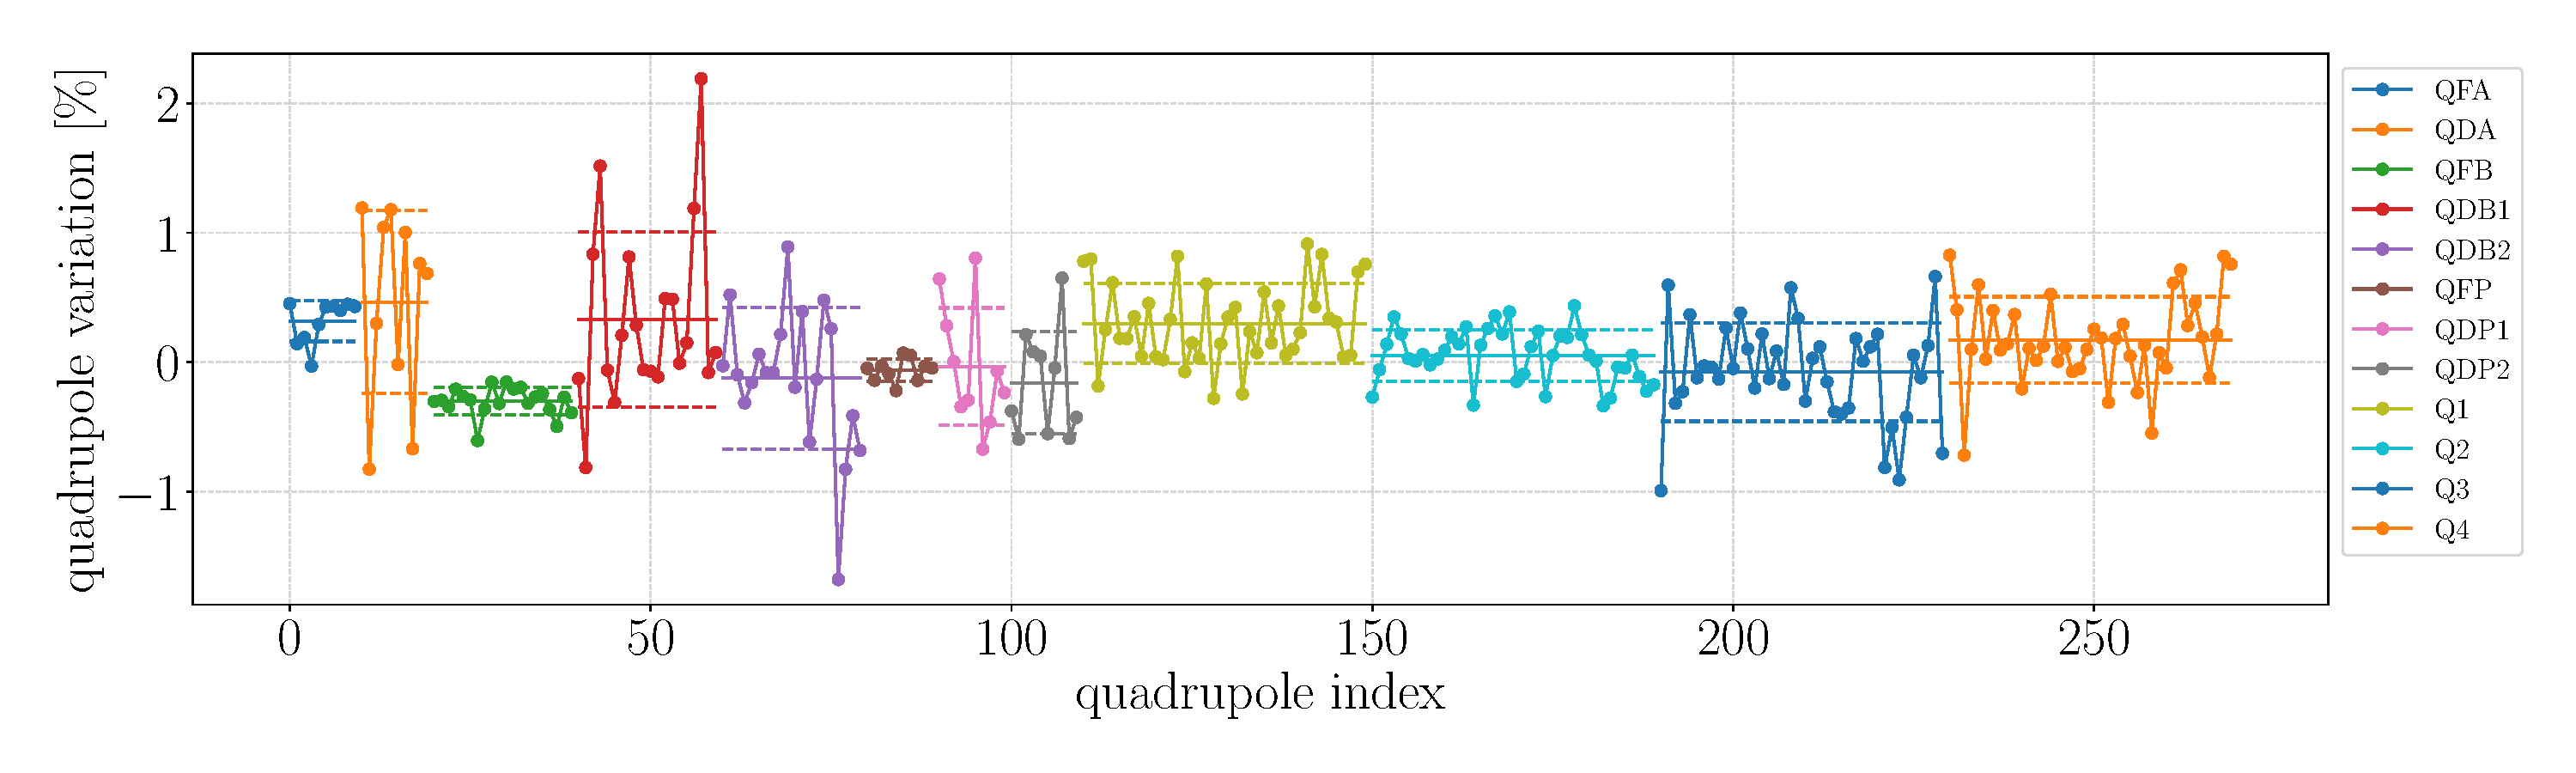
\includegraphics[width=1.0\textwidth]{figures/final_quads_correction_families_fix.pdf}
\caption{Quadrupoles families final variations after two LOCO iterations. The continuous lines indicate the family average variation and the dashed lines correspond to $\pm$ std.}
\label{fig:loco_corrections_final_families}
\end{figure}
\begin{table}[h!]
    \centering
    \caption{Quadrupole families corrections.}
    \label{tab:quad_fam_corr}
    \begin{tabular}{cccc}
        \toprule\toprule
        Quad. Family & mean [\%] & std [\%] & peak-to-valley [\%] \\
        \hline
        QDA  &  0.45  & 0.71 & 2.02 \\
        QDB1 &  0.31  & 0.68 & 3.00 \\
        QDB2 &  -0.14 &  0.55&  2.57 \\
        QDP1 &  -0.05 &  0.45 &  1.48 \\
        QDP2 &  -0.18 &  0.39 &  1.25 \\
        \hline
        QFA  &  0.31  & 0.16 & 0.48 \\
        Q1   &  0.30  & 0.31 & 1.19 \\
        Q2   &  0.05  & 0.20 & 0.77 \\
        Q3   &  -0.08 &  0.38 &  1.66 \\
        Q4   &  0.17  & 0.33 & 1.55 \\
        \hline
        QFB  &  -0.31 & 0.11 &  0.45 \\
        QFP  &  -0.07 &  0.08 &   0.29 \\
        \bottomrule\bottomrule
    \end{tabular}
\end{table}

Mechanically, three types of quadrupoles were used in Sirius storage ring, namely Q14, Q20 and Q30. The number in the name indicates the magnet length, $\SI{14}{\cm}$, $\SI{20}{\cm}$ and $\SI{30}{\cm}$, respectively. The shorter quadrupoles, Q14, were used as defocusing quadrupoles. Q20 were used for both quadrupoles in arc sections and for focusing quadrupoles in high-beta straight sections. The longest quadrupoles, Q30, were used for focusing quadrupoles in low-beta sections, in order to provide a larger integrated gradient field to focus the betatron functions in the straights sections. The quadrupoles families information in Table~\ref{tab:quad_fam_corr} are divided with horizontal line into three groups, following each magnet type to which each family corresponds. 

It can be observed that Q30 quadrupoles, QFB and QFP, presented the smaller variations, followed by Q20 and Q14 types, which are the defocusing quadrupoles, presented the largest variations. At the time of writing, the reason for these differences was not clearly understood. The LNLS Magnet Group were performing new magnetic characterizations and analysis with the quadrupoles available in the measurement laboratory to investigate the question in collaboration with LNLS~\gls{fac}.

\subsection{Calibrated Model Parameters}
Once the measured~\gls{orm} is adjusted, with the obtained calibrated model one can calculate lattice functions (beta and dispersion) and global parameters, such as betatron tunes and emittances. If the model describes accurately the real machine, this provides an indirect estimate of corresponding actual parameters.

A function that is related to the storage ring linear optics errors and asymmetries is the betatron function relative error $\Delta \beta(s)/\beta(s)$, called beta-beating. The beta-beating is a $s$-dependent function but it is common to use its standard deviation value as a characteristic parameter for the optics error level. The dispersion function~\gls{std} deviation from nominal values is a usual parameter to indicate the optics error as well.

In Table~\ref{tab:calibrated_optics}, the~\gls{std} values for beta-beating and dispersion errors are shown for each LOCO fitting.
\begin{table}[h!]
    \centering
    \caption{Lattice functions errors from calibrated model throughout LOCO fittings.}
    \label{tab:calibrated_optics}
    \begin{tabular}{ccccc}
        \toprule\toprule
        Parameter (std) & fitting \#1 & fitting \#2 & fitting \#3 & Unit \\
        \hline
        $\Delta\beta_x/\beta_x$ & \num{11.2} & \num{1.3} & \num{1.1} &\SI{}{\%}  \\
        $\Delta\beta_y/\beta_y$ & \num{7.9} & \num{0.9} & \num{1.6} &\SI{}{\%} \\
        $\Delta\eta_x$ &  \num{10.1} &  \num{1.6} & \num{1.4} & \SI{}{\milli\meter}  \\
        $\Delta\eta_y$ &  \num{3.1} &  \num{1.4} & \num{0.5} & \SI{}{\milli\meter} \\
        \bottomrule\bottomrule
    \end{tabular}
\end{table}

The results in Table~\ref{tab:calibrated_optics} indicate that $\Delta\beta_x/\beta_x$ in the calibrated models could be reduced by one tenth of its initial value. $\Delta\beta_y/\beta_y$ was reduced by a factor 5. The reduction factors for horizontal and vertical dispersion errors were $7$ and $6$, respectively.

From the calibrated model, the calculated fractional tunes agreed quite well with the measured ones as can be seen in Table~\ref{tab:calibrated_tunes}. The differences between the measured and predicted tunes from LOCO are on the order of $\num{1e-3}$ for both planes.
\begin{table}[h!]
    \centering
    \caption{Predicted fractional tunes from calibrated model compared to the measured ones for each LOCO fitting.}
    \label{tab:calibrated_tunes}
    \begin{tabular}{cccc}
        \toprule\toprule
        Parameter & fitting \#1 & fitting \#2 & fitting \#3 \\
        \hline
        measured $\nu_x$ & \num{7.6e-2} & \num{7.6e-2} & \num{7.6e-2} \\
        model $\nu_x$ & \num{7.9e-2} & \num{7.5e-2} & \num{7.5e-2}  \\
        $|\Delta \nu_x|$ & \num{3e-3} & \num{1e-3} & \num{1e-3}  \\
        \hline
        measured $\nu_y$ & \num{1.34e-1} & \num{1.38e-1} & \num{1.36e-1} \\
        model $\nu_y$ & \num{1.35e-1} & \num{1.37e-1} & \num{1.33e-1}  \\
        $|\Delta \nu_y|$ & \num{1e-3} & \num{1e-3} & \num{3e-3}  \\
        \bottomrule\bottomrule
    \end{tabular}
\end{table}

Finally, with the calibrated models the emittances were also calculated and the results are presented in Table~\ref{tab:calibrated_emittances}.
\begin{table}[h!]
    \centering
    \caption{Emittances from calibrated model throughout LOCO fittings.}
    \label{tab:calibrated_emittances}
    \begin{tabular}{ccccc}
        \toprule\toprule
        Parameter & fitting \#1 & fitting \#2 & fitting \#3 & Unit \\
        \hline
        $\epsilon_0$ & \num{283.4} & \num{250.4} & \num{251.6} & \SI{}{\pico\meter\radian}  \\
        $\epsilon_x$ & \num{280.7} & \num{250.0} & \num{251.5} & \SI{}{\pico\meter\radian} \\
        $\epsilon_y$ &  \num{2.65} &  \num{0.37} & \num{0.07} & \SI{}{\pico\meter\radian}  \\
        $\epsilon_y/\epsilon_x$ &  \num{0.94} &  \num{0.15} & \num{0.03} & \SI{}{\%} \\
        \bottomrule\bottomrule
    \end{tabular}
\end{table}

Initially the model indicated that the natural emittance was $13\%$ higher than the nominal value of $\SI{251}{\pico\meter\radian}$. The vertical emittance generated an emittance coupling ratio of $0.94\%$. The natural emittance obtained with the final calibrated model was very close to the nominal and the vertical emittance was virtually absent.

\section{Independent Measurements}\label{sec:independent_meas}
There are some measurements that can be realized to check independently the impact of LOCO corrections in Sirius storage ring. Lattice functions, betatron and dispersion, are measured to verify the machine linear optics and its deviations to the nominal functions. Measuring the avoided-crossing in betatron tunes provides the information about the global betatron coupling. To check the performance in beam dynamics, one can measure the dynamic aperture and injection efficiency, two typically correlated quantities. When these studies were performed, the Sirius diagnostic beamline was not installed yet, so it was not possible to perform beam size and emittance measurements.

\subsection{Dispersion Function}
The information about dispersion function is already encoded in one of~\gls{orm} columns. A column of this matrix is the orbit response due to a variation in~\gls{rf} frequency. From Eq.~\eqref{eq:rf_column}, the dispersion function at BPMs positions can be calculated as:
\begin{equation}
\eta_u(s_i) = -\alpha f_{\mathrm{rf}}\dfrac{\Delta u_i}{ \Delta f_{\mathrm{rf}}},
\end{equation}
where $u=x, y$ and $\alpha$ is the momentum compaction factor. Thus, given the~\gls{rf} frequency used in~\gls{orm} measurements, the dispersion is obtained with the corresponding~\gls{orm} column.

In this case, the dispersion function is not exactly an independent measurement, since it is included in LOCO fitting. For Sirius, it was required to include a weight factor to force the matching between measured and calculated dispersion function. It was tested that if this factor was not used, the measured~\gls{orm} were adjusted except for dispersion column. Applying the gradients variations calculated by LOCO actually increased $\eta(s)$ errors, specially on vertical plane. On the other hand, if the weight factor was further increased, the measured $\eta(s)$ is better explained with the model however the~\gls{orm} fitting quality was lowered.

With the measured~\gls{orm}s before and after LOCO corrections, $\eta_x$ and $\eta_y$ at~\glspl{bpm} were calculated and compared with the nominal function. The results are shown in Figure~\ref{fig:disp_error}. 
\begin{figure}
\centering
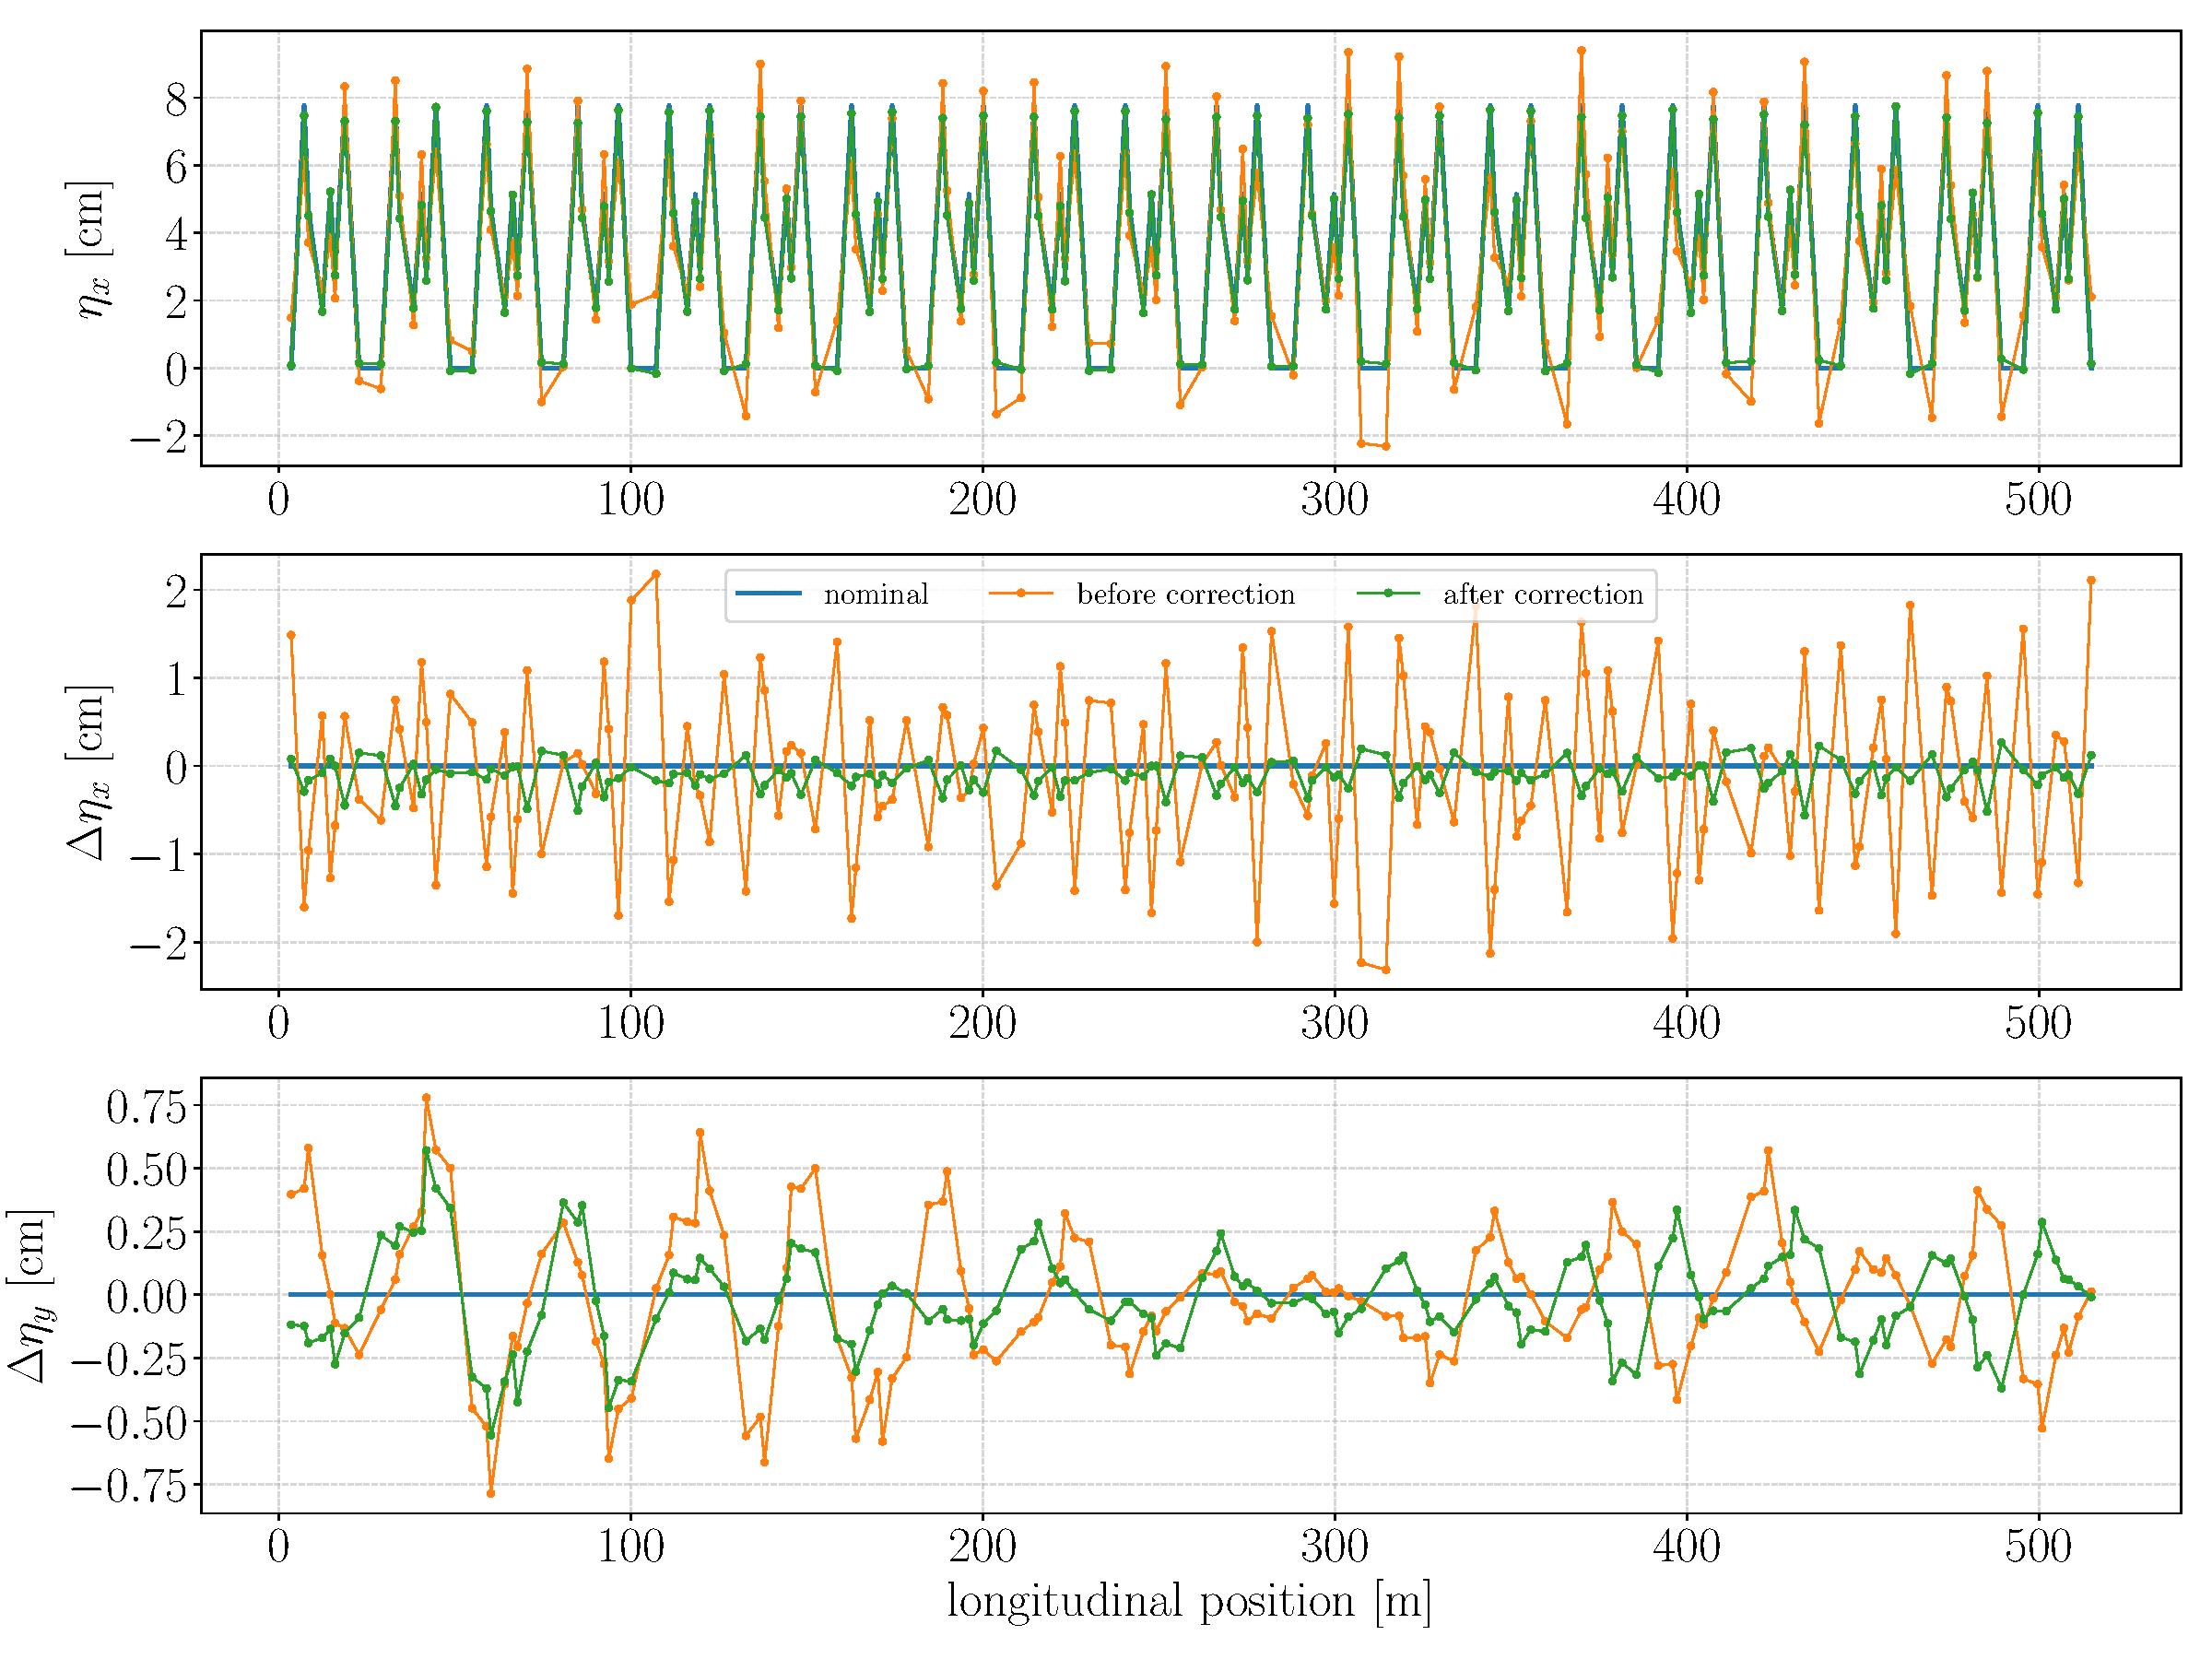
\includegraphics[width=1.0\textwidth]{figures/dispersion_after_before_loco_legend.pdf}
\caption{Measured dispersion functions on BPMs and its differences from nominal values.}
\label{fig:disp_error}
\end{figure}

It can be observed that the horizontal dispersion errors were greatly reduced, specially in straight sections, were $\eta_x = 0$ nominally. However, the errors of vertical dispersion could not be reduced with the same effectiveness. This was already expected, since the LOCO calibrated models predicted $\eta_y$ functions very different from the measured ones. Initially the std error for $\eta_x$ was $\SI{10.2}{\milli\meter}$ and after the corrections it was reduced to $\SI{1.6}{\milli\meter}$. For $\eta_y$, these errors were $\SI{2.8}{\milli\meter}$ before and $\SI{1.9}{\milli\meter}$ after LOCO. From Table~\ref{tab:calibrated_optics}, it is seen that LOCO model accurately predicted the values obtained in the real storage ring for $\eta_x$. On the other hand, even tough the initial predicted and measured  $\eta_y$ are in concordance, the final $\eta_y$ error calculated with the calibrated model is about 4 times lower than the corresponding measured error. This incompatibility will be further discussed in Section~\ref{sec:orbit_effect}.

\subsection{Betatron Function}
In Subection~\ref{subsec:optics} it is discussed how gradient errors perturb the linear optics on a storage ring. In Appendix~\ref{appendix:beta} the effect of a single gradient error in a quadrupole of length $L$ on the betatron tunes, given the beta function, is calculated. The process can be reversed: intentionally changing the integrated gradient of a single quadrupole by a small amount $\Delta \mathrm{KL}$ and measuring the corresponding tune shift, the integral of beta function along the quadrupole is calculated simply as:
\begin{align}
\dfrac{1}{L}\int_{0}^{L} \beta_u(s) \mathrm{d}s &= 4\pi\frac{\Delta \nu_u}{\Delta \mathrm{KL}},
\end{align}
where $u=x, y$. This method has the disadvantage that the gradient variation $\Delta \mathrm{KL}$ applied in the quadrupole must be well known, otherwise this will introduce systematic errors in beta calculation. Since the tunes measurements are typically very precise, the error in the determination of $\Delta \nu_u$ is negligible to the beta measurement.

This process, which will be called beta measurement by tune shifts, can be performed in every quadrupole to measure the betatron functions around the storage ring. Then, the obtained values may be compared to the nominal ones, which can be obtained in the model numerically, simulating the described process, or by analytical calculations of these integrals, as shown in Appendix~\ref{appendix:beta}.

The author implemented the beta measurement by tunes shifts for Sirius storage ring in a Python script and the code can be accessed in its GitHub Repository~\cite{betasirius}. The script also performs the data analysis and evaluates the beta integrals for a given Sirius storage ring model, returning both measured and model beta integrals at quadrupoles for comparison.

The measurement process were tested and adjusted several times. After 10~\gls{orm}s were measured to obtain the fit parameters variations as discussed in Subsection~\ref{subsec:fit_var}, 10 sequential beta measurements were performed as well. Calculating the dispersion function from the 10 measured~\gls{orm}s, the variations for lattice functions measurements in Sirius storage ring were obtained and the results are organized in Table~\ref{tab:twiss_var_meas}. 
\begin{table}[h!]
    \centering
    \caption{Variations in lattice functions for 10 sequential measurements performed in Sirius storage ring.}
    \label{tab:twiss_var_meas}
    \begin{tabular}{cccc}
        \toprule\toprule
        Lattice function & std variation & peak-to-valley variation & Unit \\
        \hline
        $\beta_x$ & \num{0.8}& \num{4.3} & \%\\
        $\beta_y$ & \num{0.5} & \num{4.2}& \% \\
        $\eta_x$ & \num{0.2} & \num{0.9} & \SI{}{\milli\meter}\\
        $\eta_y$ & \num{0.3} & \num{1.3} & \SI{}{\milli\meter} \\
        \bottomrule\bottomrule
    \end{tabular}
\end{table}

The~\gls{std} variations for each point were used to define the related error bars, which is this case are related to random errors. Notice that dispersion function measurement variations are low, due to the fact that~\gls{rf} frequency changes are precise and well known. On the other hand, variations in beta measurement on the order of few percent. The main cause for this is hysteresis in the quadrupoles gradient fields. It is desirable to correct the storage ring linear optics in the level of measurements errors.

The implemented script was applied to obtain the Sirius beta functions before and after the application of LOCO corrections in quadrupoles trim-coils and the results are shown in Figure~\ref{fig:beta_tuneshift}. The corresponding beta-beatings for the absolute measured values are plotted in Figure~\ref{fig:beta_beating_progress}.
\begin{figure}
\centering
\begin{subfigure}[t]{0.49\textwidth}
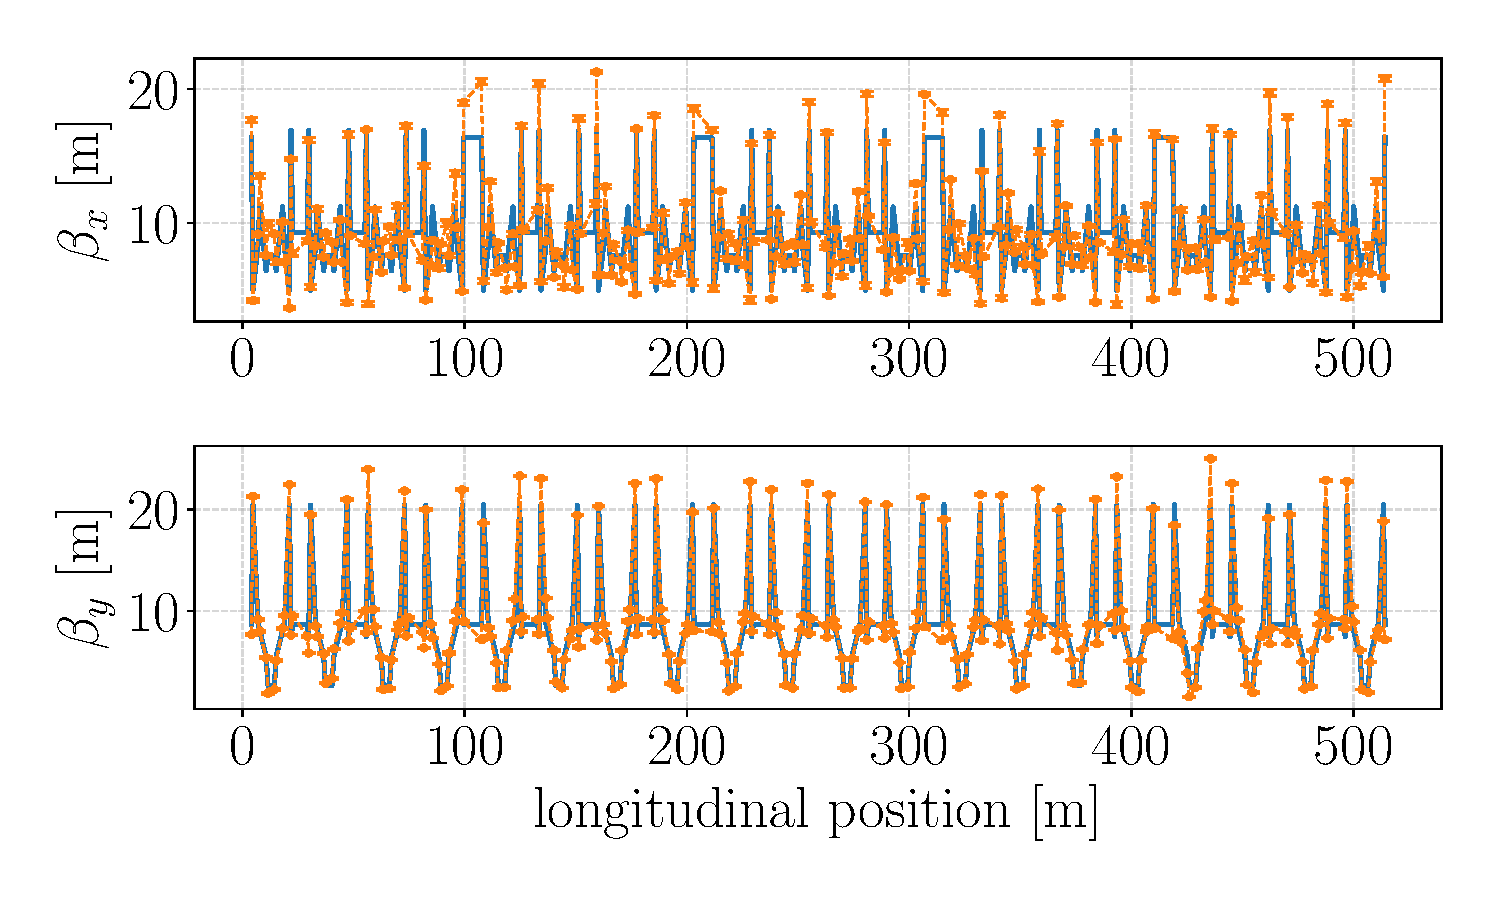
\includegraphics[width=1.0\textwidth]{figures/beta_before_big.pdf}
    \caption{Before.}
    \label{subfig:beta_before}
\end{subfigure}
 \begin{subfigure}[t]{0.49\textwidth}
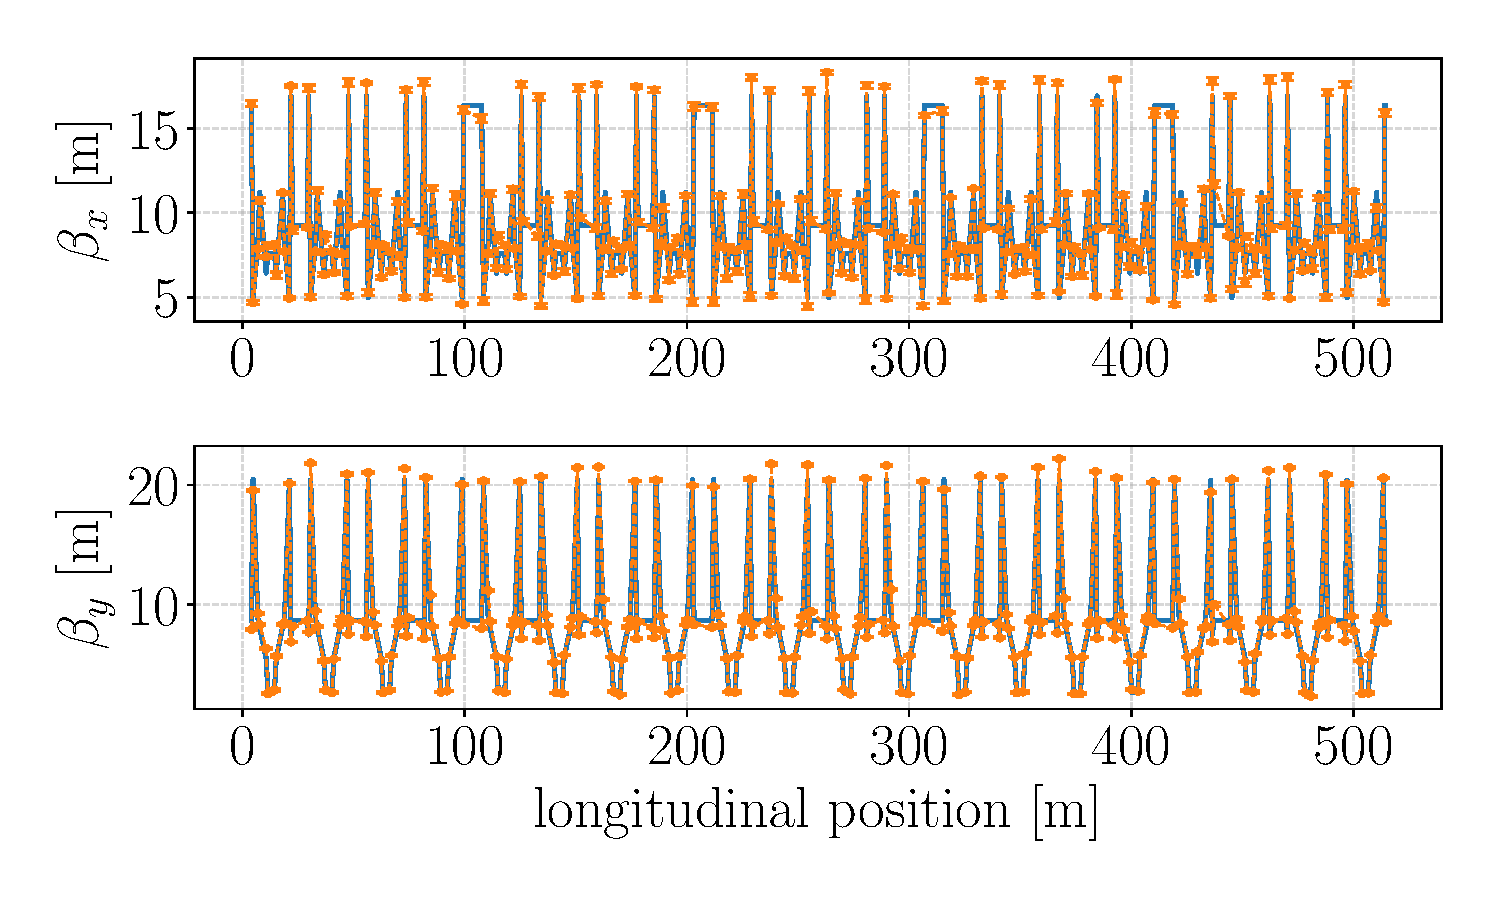
\includegraphics[width=1.0\textwidth]{figures/beta_after_big.pdf}
    \caption{After.}
    \label{subfig:beta_after}
\end{subfigure}
\caption{Nominal (blue) and measured (orange) betatron functions before and after LOCO corrections.}
\label{fig:beta_tuneshift}
\end{figure}
\begin{figure}
\centering
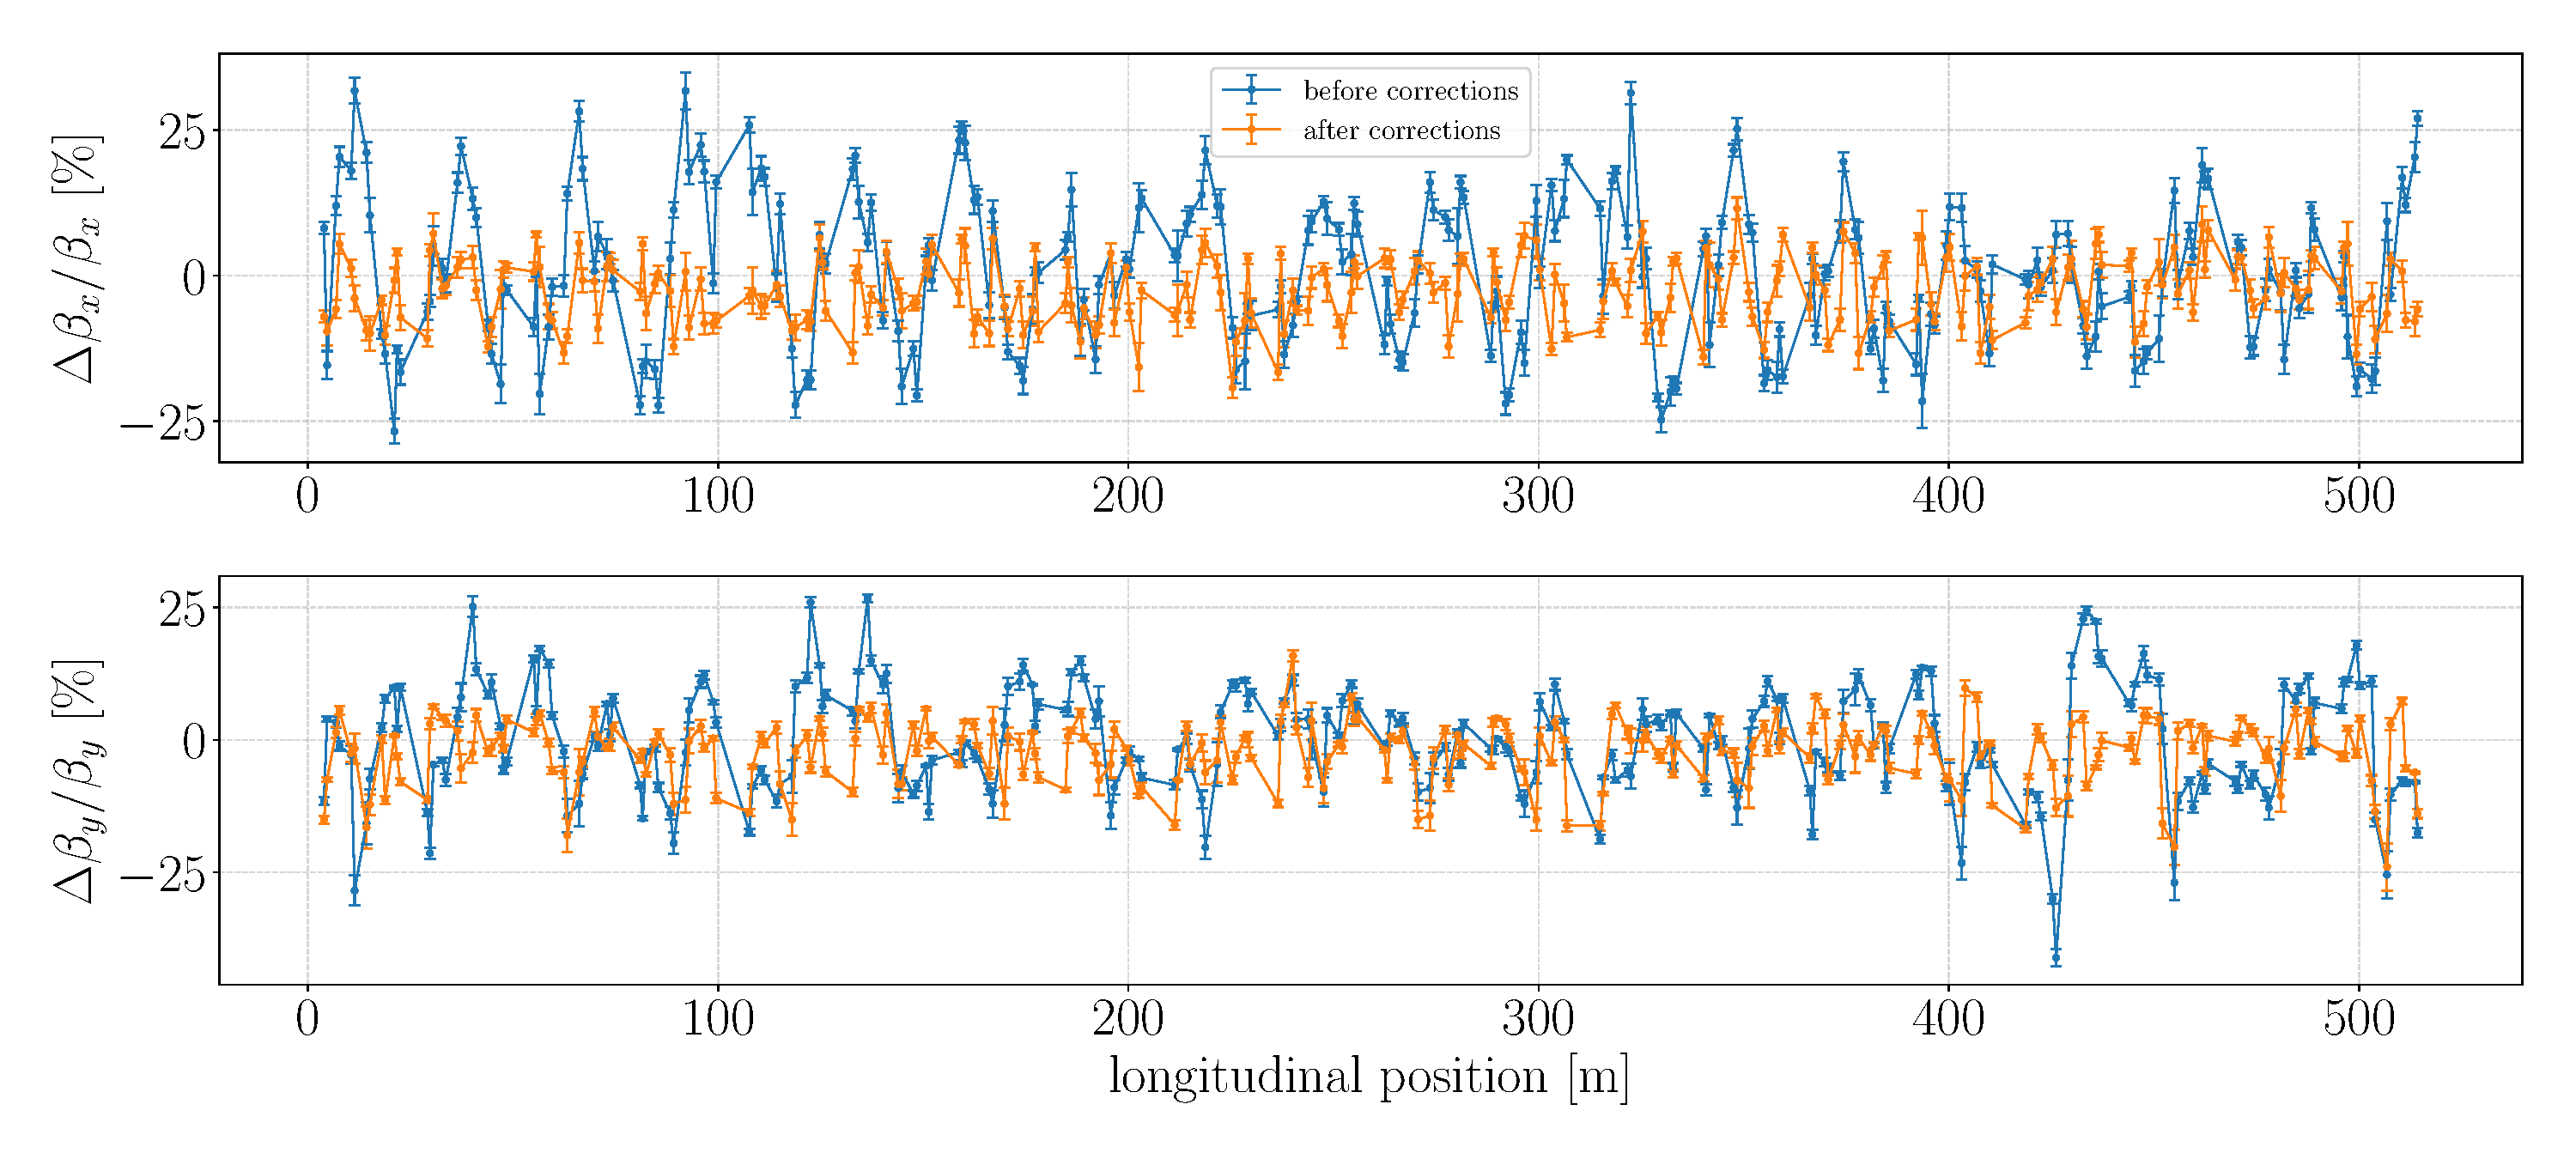
\includegraphics[width=1.0\textwidth]{figures/beta_beating_progress_big.pdf}
\caption{Comparsion of beta-beating before and after optics corrections.}
\label{fig:beta_beating_progress}
\end{figure}

Before LOCO corrections, measured horizontal and vertical beta-beatings (std) were $\SI{12.8(8)}{\%}$ and $\SI{10.4(5)}{\%}$, respectively. With new gradients settings these values were reduced to $\SI{3.9(8)}{\%}$ and $\SI{4.1(5)}{\%}$.

An alternative method to measure beta functions can be realized by applying~\gls{pca} in~\gls{tbt} position measurements from~\glspl{bpm}. The beam orbit can be perturbed with a dipolar impulse, applied by an element in storage ring called pinger, exciting betatron oscillations that are acquired by~\glspl{bpm}. The various oscillation harmonics BPM data can be identified and separated with~\gls{pca}. The two main components for each plane of oscillation are related to the betatron motion and from this main harmonics it is possible to extract the beta functions and the phase advances in BPMs. For more details about the method, the author recommends the reference~\cite{huang2019beam}.

In Sirius storage ring, the dipolar kicker, used for on-axis injection, can also be used as a horizontal pinger. When these measurements were conducted, a vertical pinger was not available, so it was possible to measured only the horizontal beta function in~\glspl{bpm} via~\gls{pca} method. These measurements were realized before and after LOCO corrections, using a small kick impulse of $\SI{100}{\micro\radian}$ and analysing the~\gls{tbt} data for 4000 turns. The horizontal beta-beatings obtained were compared with measurements at quadrupoles by tune shifts and with the predicted beta-beating from LOCO calibrated models. These results are plotted in Figure~\ref{fig:betax_compare}.
\begin{figure}
\centering
\begin{subfigure}[t]{1.0\textwidth}
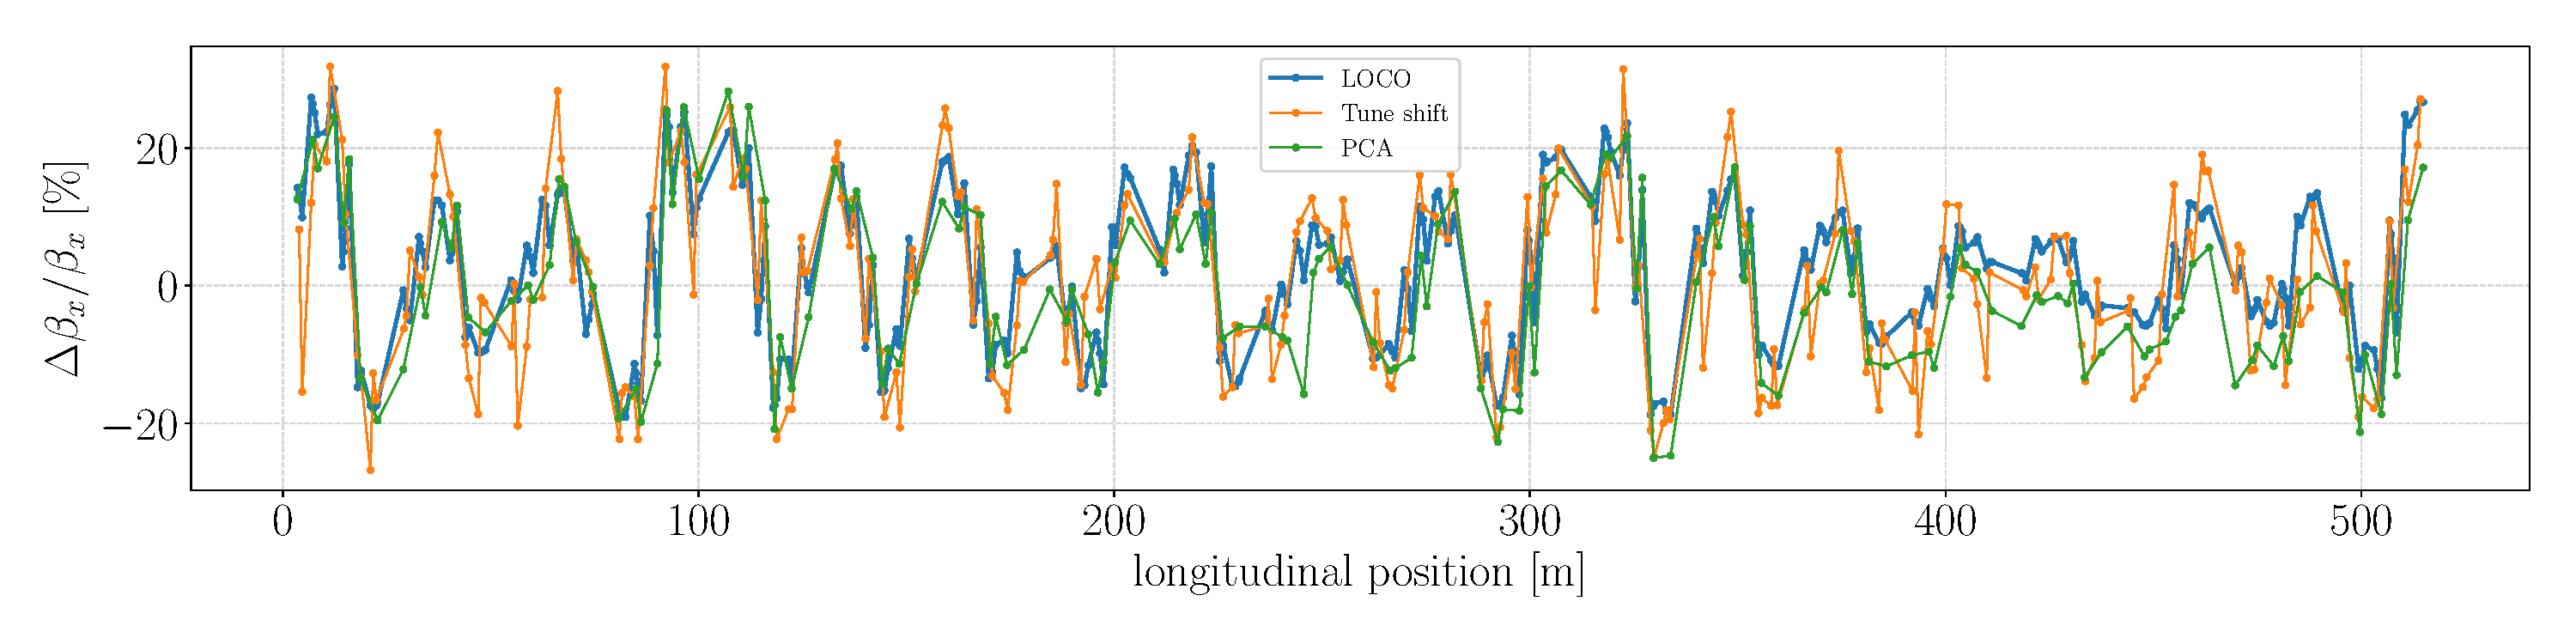
\includegraphics[width=1.0\textwidth]{figures/betax_compare_loco_pca_quad_before_corr.pdf}
    \caption{Before correction.}
    \label{subfig:betax_compare_before}
\end{subfigure}
 \begin{subfigure}[t]{1.0\textwidth}
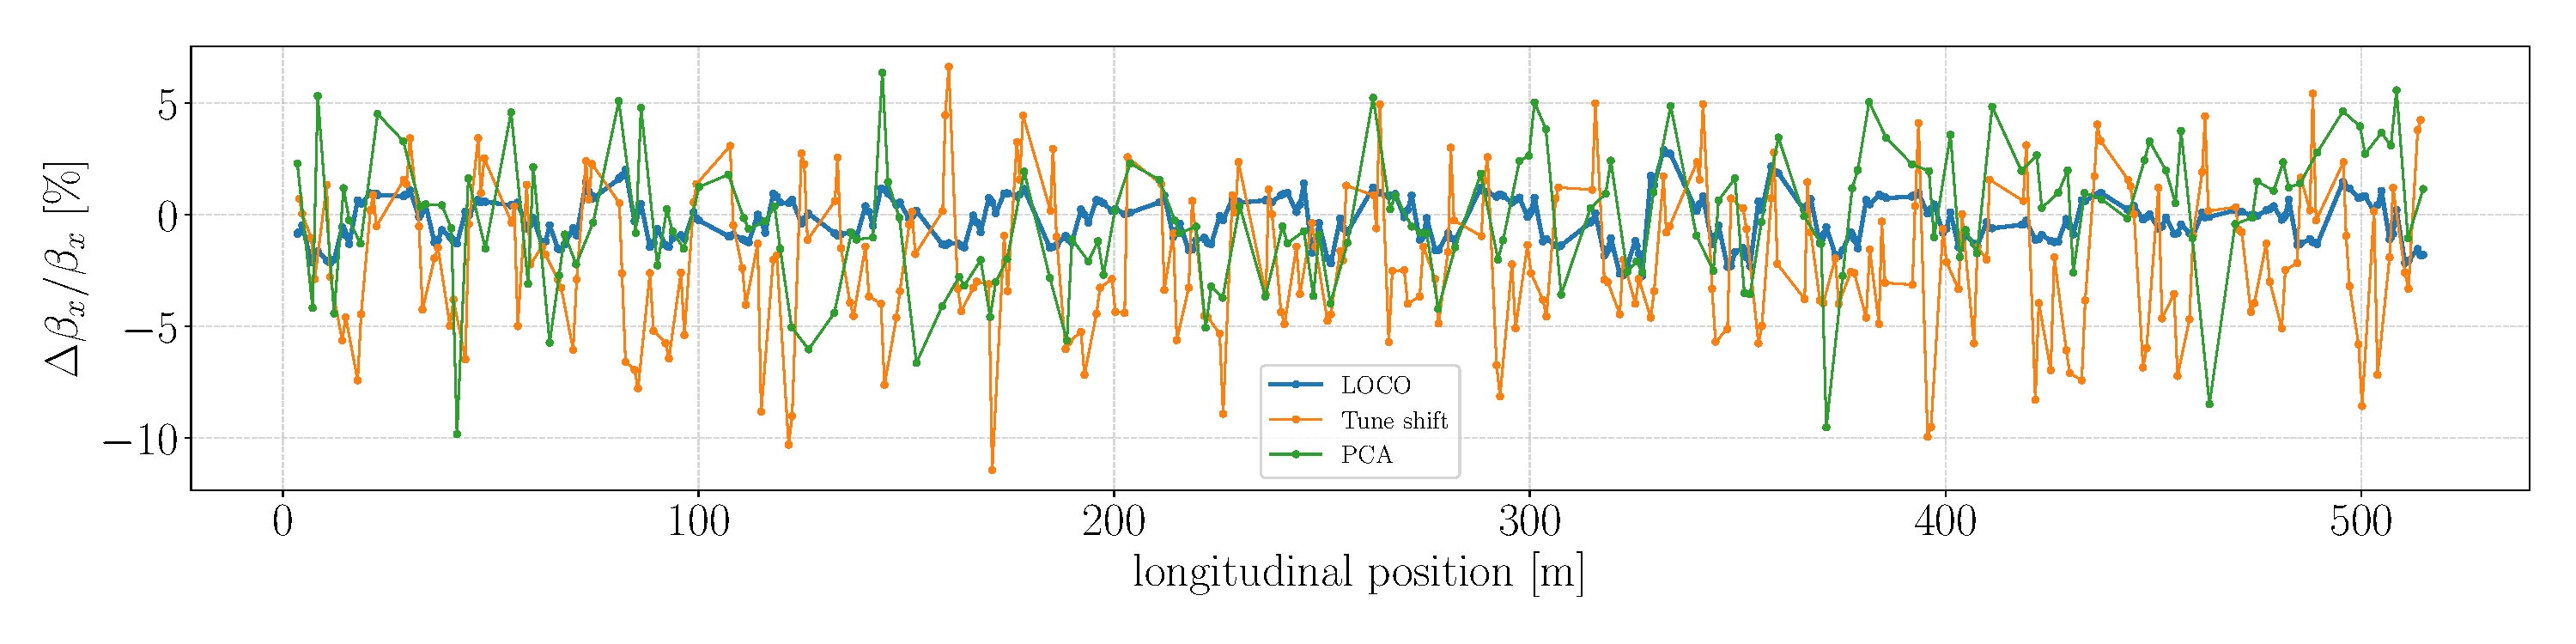
\includegraphics[width=1.0\textwidth]{figures/betax_compare_loco_pca_quad_after_corr.pdf}
    \caption{After correction.}
    \label{subfig:betax_compare_after}
\end{subfigure}
\caption{Horizontal beta-beating comparison between predicted beta with LOCO model and beta measurements: at quadrupole based on tune shifts and at BPMs based on PCA applied on turn-by-turn data.}
\label{fig:betax_compare}
\end{figure}

Before LOCO corrections, the three measurements agreed quite well. The correlation between LOCO and PCA beta-beating signatures is $91\%$ and between LOCO and tune shifts is $86\%$. On the other hand, it can be seen that after the corrections, the LOCO model fails to predict the measured beta-beating in storage ring. In this situation, the correlation between LOCO and PCA values is $39\%$ and LOCO and tune shifts it is only $8\%$. The same is valid for~\gls{std} beta-beating, before corrections the values were; LOCO: $\SI{11.3}{\%}$, tune shift: $\SI{12.8}{\%}$, PCA: $\SI{11.5}{\%}$ and after corrections; LOCO: $\SI{1.0}{\%}$, tune shift: $\SI{3.3}{\%}$, PCA: $\SI{3.0}{\%}$. Then, in the latter case, the calibrated model predicted a horizontal beta-beating that is 3 times smaller than the measured values in Sirius storage ring.

% before: peak-to-valley x 58.6 y 67.9
% before: max abs x 31.8 y 41.1
% \\
% after: peak-to-valley x 36.9, y 38.8
% after  max abs x 26.4 y 26.8
\subsection{Betatron Coupling}
In Subection~\ref{subsec:linear_coupling} the effect of skew gradients on betatron coupling was briefly discussed. It was shown that a global parameter $|\kappa|$, called global betatron coupling, can be measured by approximating the betatron tunes, taking advantage on the fact that the tune difference resonance is stable. In the presence of coupling, the transverse tunes $\nu_x$ and $\nu_y$ are replaced by two normal tunes $\nu_1$ and $\nu_2$, also called eigentunes. This coupling problem can be formulated to be mathematically equivalent to the avoided crossing problem in a two-level system in quantum mechanics. In this case, the matrix $\mathbf{C} = \begin{bmatrix} \nu_x & \kappa \\ \kappa & \nu_y \end{bmatrix}$ takes the place of the two-state hamiltonian and its eigenvalues are calculated:
\begin{align}
    \nu_1 &= \dfrac{\nu_x + \nu_y}{2} + \dfrac{1}{2}\sqrt{\left(\dfrac{\nu_x - \nu_y}{2}\right)^2 + 4 \kappa^2}, \\
    \nu_2 &= \dfrac{\nu_x + \nu_y}{2} - \dfrac{1}{2}\sqrt{\left(\dfrac{\nu_x - \nu_y}{2}\right)^2 + 4 \kappa^2}.
    \label{eq:normal_tunes}
\end{align}

The equations above are equivalent to Eq.~\eqref{eq:eigentunes}. In the limit $\nu_x = \nu_y$, we also obtain that $\nu_1 - \nu_2 = |\kappa|$.

The tunes approximation can be performed by changing the focusing strengths in the storage ring. For Sirius, the fractional horizontal tune is lower than the vertical tune, thus the value scan be approximated by increasing a focusing quadrupole strength. The QFB family was chosen for this experiment. If the power supply current that feeds this quadrupole family is changed by $\Delta I_{\mathrm{QFB}}>0$, there will be a corresponding change in horizontal tune $\Delta\nu_x > 0$ and vertical tunes $\Delta\nu_y < 0$. In this way, both the tune sum and difference can be viewed as function of QFB current: $\nu_x + \nu_y = \Sigma \nu_{x, y} = f\left(I_{\mathrm{QFB}}\right)$ and $\nu_x - \nu_y = \Delta \nu_{x, y} = g\left(I_{\mathrm{QFB}}\right)$.

The measurement script and analysis was implemented by an~\gls{fac} colleague and used by the author in Sirius storage ring to obtain the global betatron tunes before and after LOCO corrections. The results are shown in Figure~\ref{fig:global_coupling}. The fitting gray curve presented in Figure~\ref{fig:global_coupling} were obtained by plugging the measured $\nu_x$, $\nu_y$ for each current $I_{\mathrm{QFB}}$ in matrix $\mathbf{C}$, diagonalizing it and finding the parameter $\kappa$ and the offsets $(\nu_x+\nu_y)/2$ that minimize the quadratic difference to the data.
\begin{figure}
\centering
\begin{subfigure}[t]{0.49\textwidth}
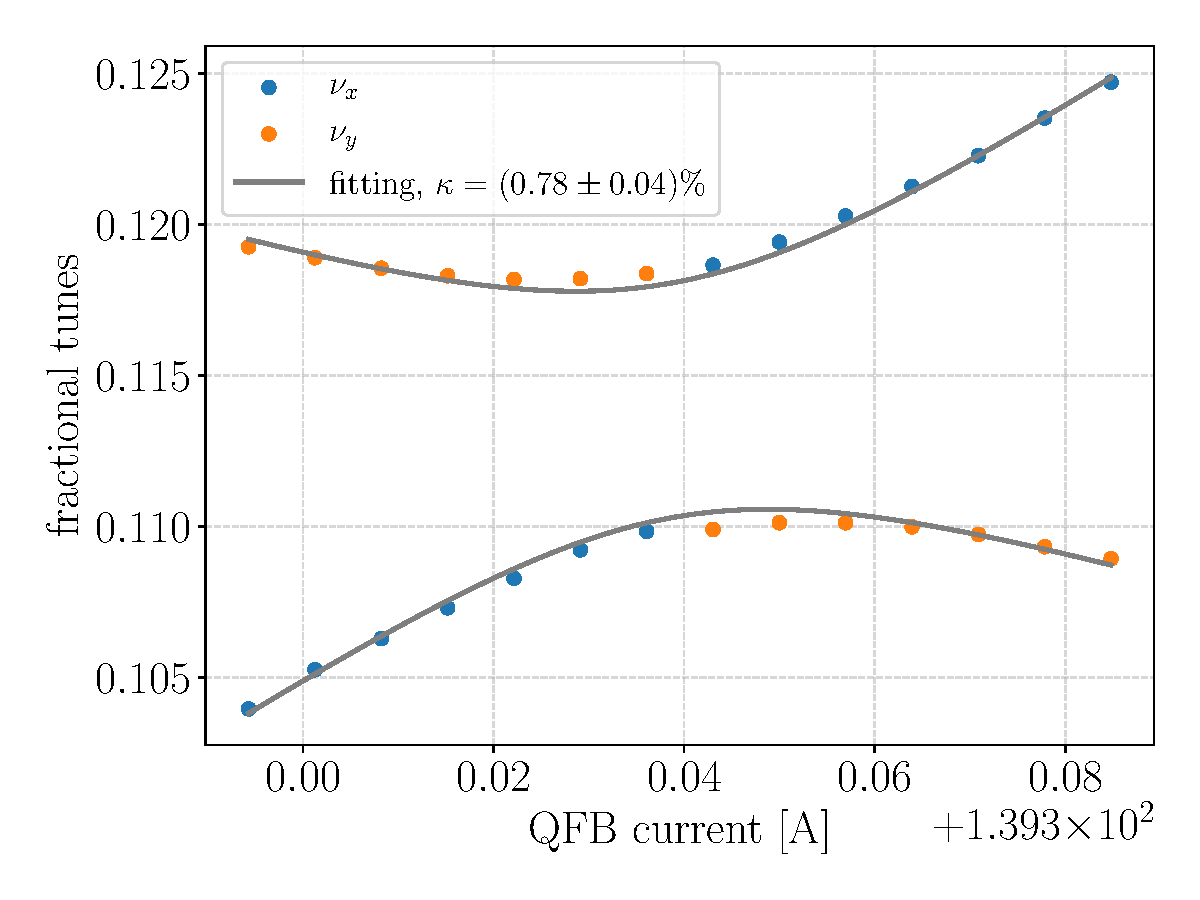
\includegraphics[width=1.0\textwidth]{figures/coupling_before_loco_grid_filter.pdf}
    \caption{Before.}
    \label{subfig:coup_before}
\end{subfigure}
 \begin{subfigure}[t]{0.49\textwidth}
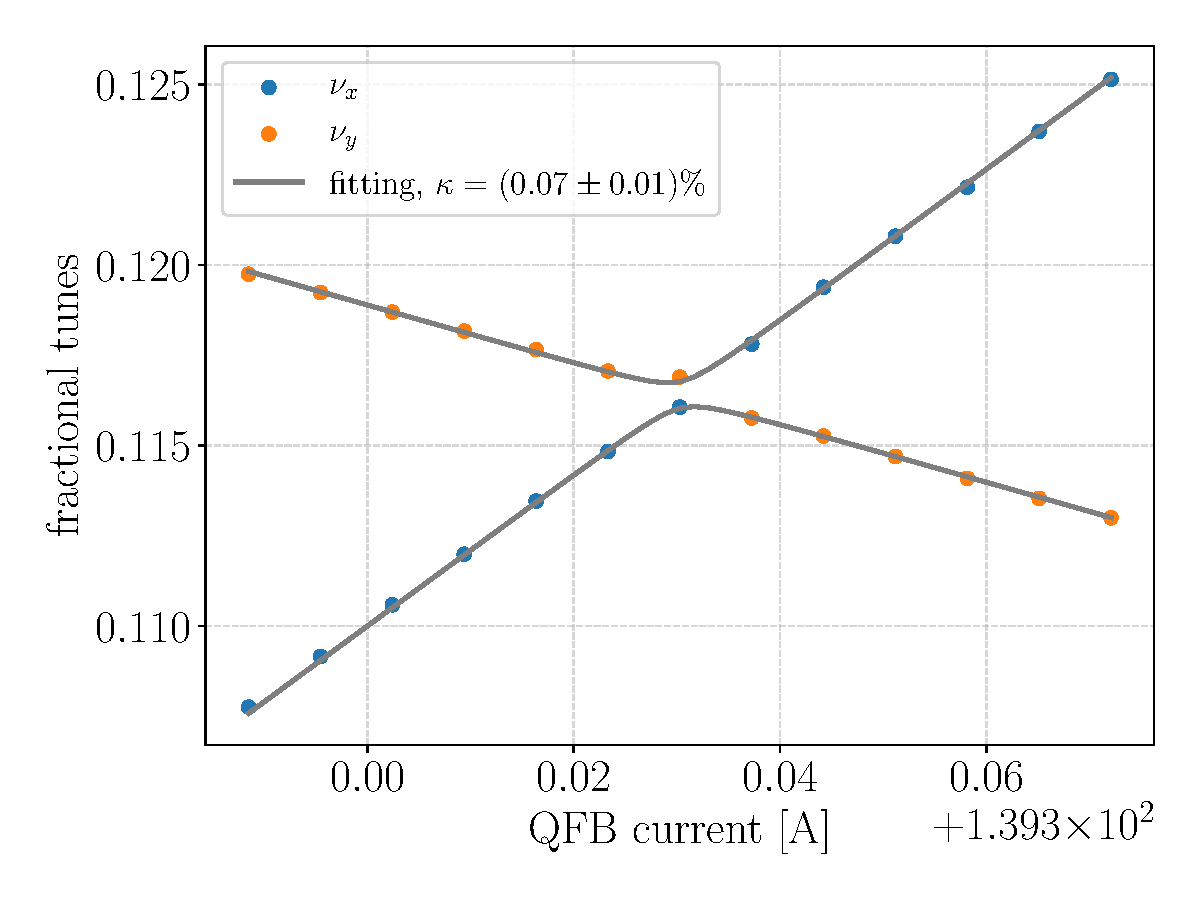
\includegraphics[width=1.0\textwidth]{figures/coupling_after_loco_grid_filter.pdf}
    \caption{After.}
    \label{subfig:coup_after}
\end{subfigure}
\caption{Global betatron coupling before and after LOCO corrections.}
\label{fig:global_coupling}
\end{figure}
In LOCO coupling corrections applied on skew quadrupoles, the residues that were used for minimization were $M_{xy}$ and $M_{yx}$, the~\gls{orm} off-diagonal elements, which are related to the local coupling along storage ring. However, the minimum tune difference measurements showed that the global betatron coupling was reduced as well, from the initial value of $\SI{0.78(4)}{\%}$ to $\SI{0.07(1)}{\%}$.

It is important to mention the goal coupling for Sirius storage ring is not necessarily zero. The coupling parameter is somewhat a free parameter that can be varied to attend other purposes, for example to increase the beam lifetime or the vertical beam size. Neverthless, a common procedure is to first reduce the betatron coupling as much as possible in the first plane then increase the coupling towards the goal value in a controlled manner. With this studies, it was proved that LOCO is a robust method to minimize the off-diagonal~\gls{orm} elements and in this process the global betatron coupling is consequently reduced. However, even tough the measured betatron coupling is near zero, since the vertical dispersion function could not be reduced with LOCO corrections, it is likely that the vertical beam emittance is still about $1\%$ of the horizontal emittance, as calculated in the first calibrated model.

\subsection{Horizontal Dynamic Aperture}

The horizontal pinger can also be used to apply dipolar impulses in the stored electron beam with increasing amplitudes until the beam is partially or totally lost. The extreme transverse positions over the turns can be acquired with~\glspl{bpm} to obtain how much beam is lost as a function of position. This is basically the dynamic aperture measurement. Since only the horizontal pinger was available in Sirius storage ring, only the horizontal dynamics aperture could be measure, before and after optics and coupling corrections. The results are presented in~\ref{fig:xdynap}.
\begin{figure}
\centering
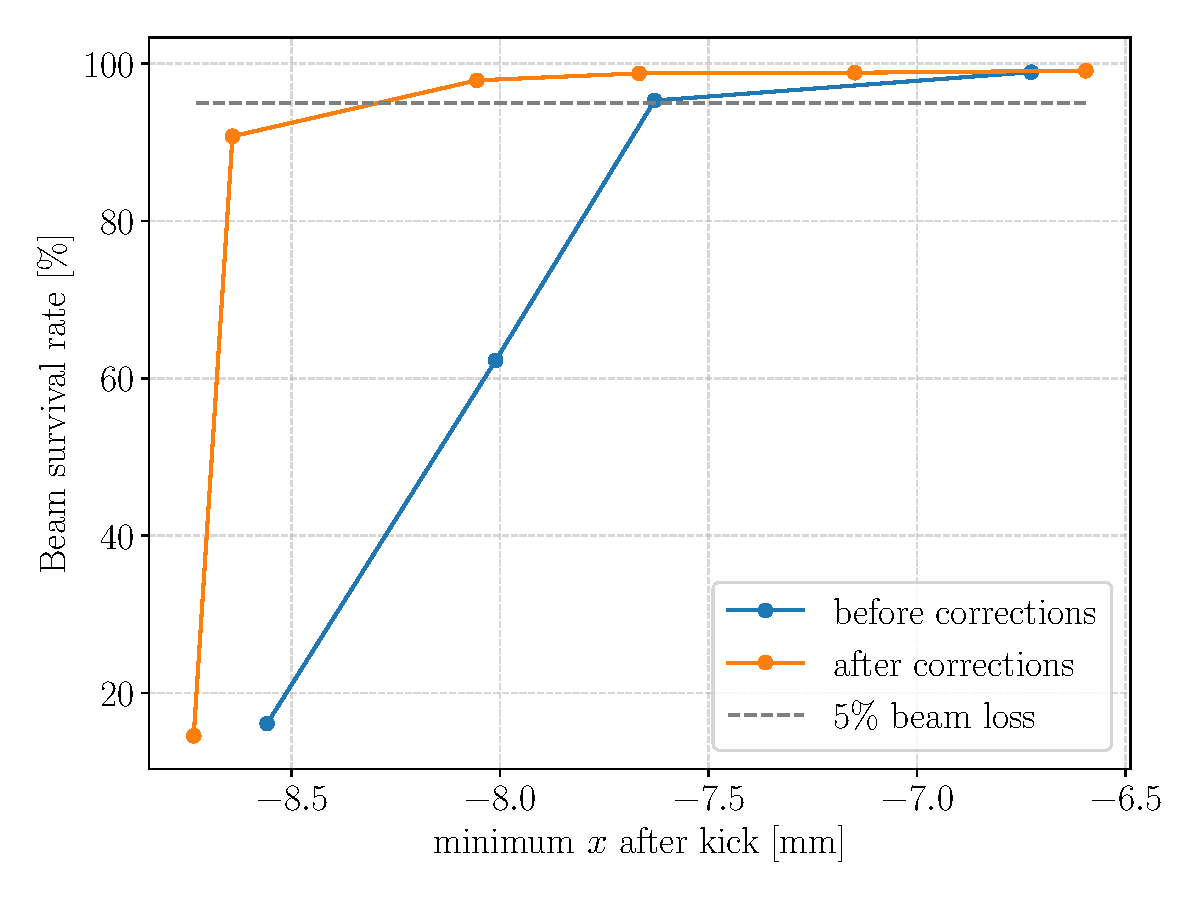
\includegraphics[width=0.75\textwidth]{figures/xdynamic_aperture_grid.pdf}
\caption{Comparison of horizontal dynamic aperture measurement before and after LOCO corrections.}
\label{fig:xdynap}
\end{figure}

Setting $5\%$ as the beam loss limit to estimate the dynamic aperture, after the application of LOCO corrections on linear optics and coupling, the horizontal dynamic aperture was increased from $\SI{7.6}{\milli\meter}$ to $\SI{8.3}{\milli\meter}$, which is an optimization of approximately $10\%$.

The horizontal dynamic aperture is important for Sirius injection, given that a non-linear kicker (NLK) is used to perform off-axis injection in the storage ring. The off-axis injection occurs at $x=\SI{-8}{mm}$ from the vacuum chamber center, because at that location the NLK field is maximum by design. The NLK field rapidly decays as the position approaches $x=0$, causing no effect on stored beam. More information about off-axis injection with NLK can be found in~\cite{liu2016a} and~\cite{wikinlk}.

To efficiently inject electron from Booster with NLK, the storage ring dynamics at $x=\SI{-8}{mm}$ must be stable. From the simulations with Sirius storage ring model, including alignment and field errors (satisfying the specifications), the dynamic aperture obtained is $x=\SI{-10}{mm}$. Therefore, even with the improvement realized with LOCO corrections, the measured horizontal dynamic aperture is still about $20\%$ lower than expected from simulations. 

It is worth to mention that beam dynamics in Sirius storage ring depend strongly on non-linear effects, which is well-known for 4\ts{th} generation light sources. At the time of writing, non-linear optimizations were not applied in Sirius yet. This kind of optimization is one example of accelerator physics studies that might improve the storage ring dynamic aperture towards design values.

\subsection{Injection Efficiency}
To close this section of independent measurements, the injection efficiency in storage ring was recorded before and after linear optics and coupling corrections. The data is presented in Figure~\ref{fig:injeff}.
\begin{figure}[h!]
\centering
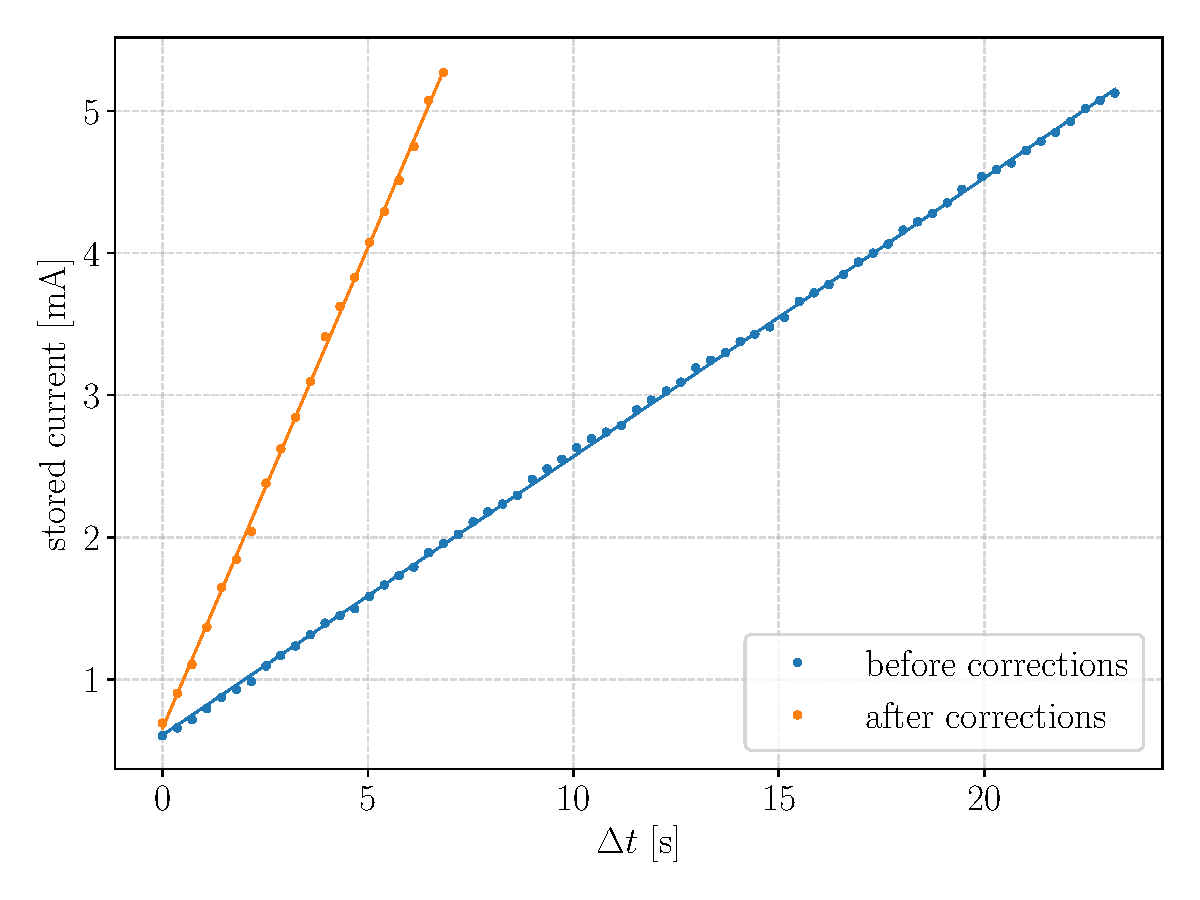
\includegraphics[width=0.75\textwidth]{figures/injeff_grid.pdf}
\caption{Beam accumulation before and after LOCO corrections.}
\label{fig:injeff}
\end{figure}

A linear fitting was applied on the data presented in Figure~\ref{fig:injeff}. The angular coefficient increased from $\SI{196}{\micro\ampere\second^{-1}}$ to $\SI{677}{\micro\ampere\second^{-1}}$. The Sirius injection rate is $\SI{2}{\hertz}$ and the current delivered by booster to the storage ring is $\SI{500}{\micro\ampere}$ on average, i.e, with an injection without any losses, the accumulation rate would be approximately $\SI{1}{\milli\ampere\second^{-1}}$. Therefore, with optics and coupling corrections, the average injection efficiency was increased from $20\%$ to $68\%$, which is an improvement of a factor $3.4$.

During the commissioning, large pulse-by-pulse variations on injection efficiency have been observed. The changes in injection efficiency recorded were as high as $20\%$. This problem might be related to the dynamic aperture, since its measured value indicates that the electron beam must be injected in the dynamic aperture edge in order to receive the required kick from NLK. In this situation, any change of a few percent in the injection condition leads to electron losses. For the top-up injection mode on Sirius, an injection efficiency higher than $95\%$ with small variation between injection pulses is required, so Sirius dynamic aperture optimization is a work in progress. 

\section{Orbit Effect on Optics and Coupling}\label{sec:orbit_effect}
Orbit correction on Sirius storage ring was performed as follows: the BPM offsets with respect to quadrupoles centers were measured to define the~\gls{bba} orbit, then this orbit is used as the target for orbit correction. In this process, it was not possible to use all 281 singular values available in~\gls{orm} in the corrections, otherwise the correctors strengths would surpass the kick limits $\pm \SI{300}{\micro\meter}$. Thus, it was necessary to use only 180 singular values in orbit correction and the final residual orbit, represented in Figure~\ref{fig:orbit_residue}, was obtained.
\begin{figure}[h!]
\centering
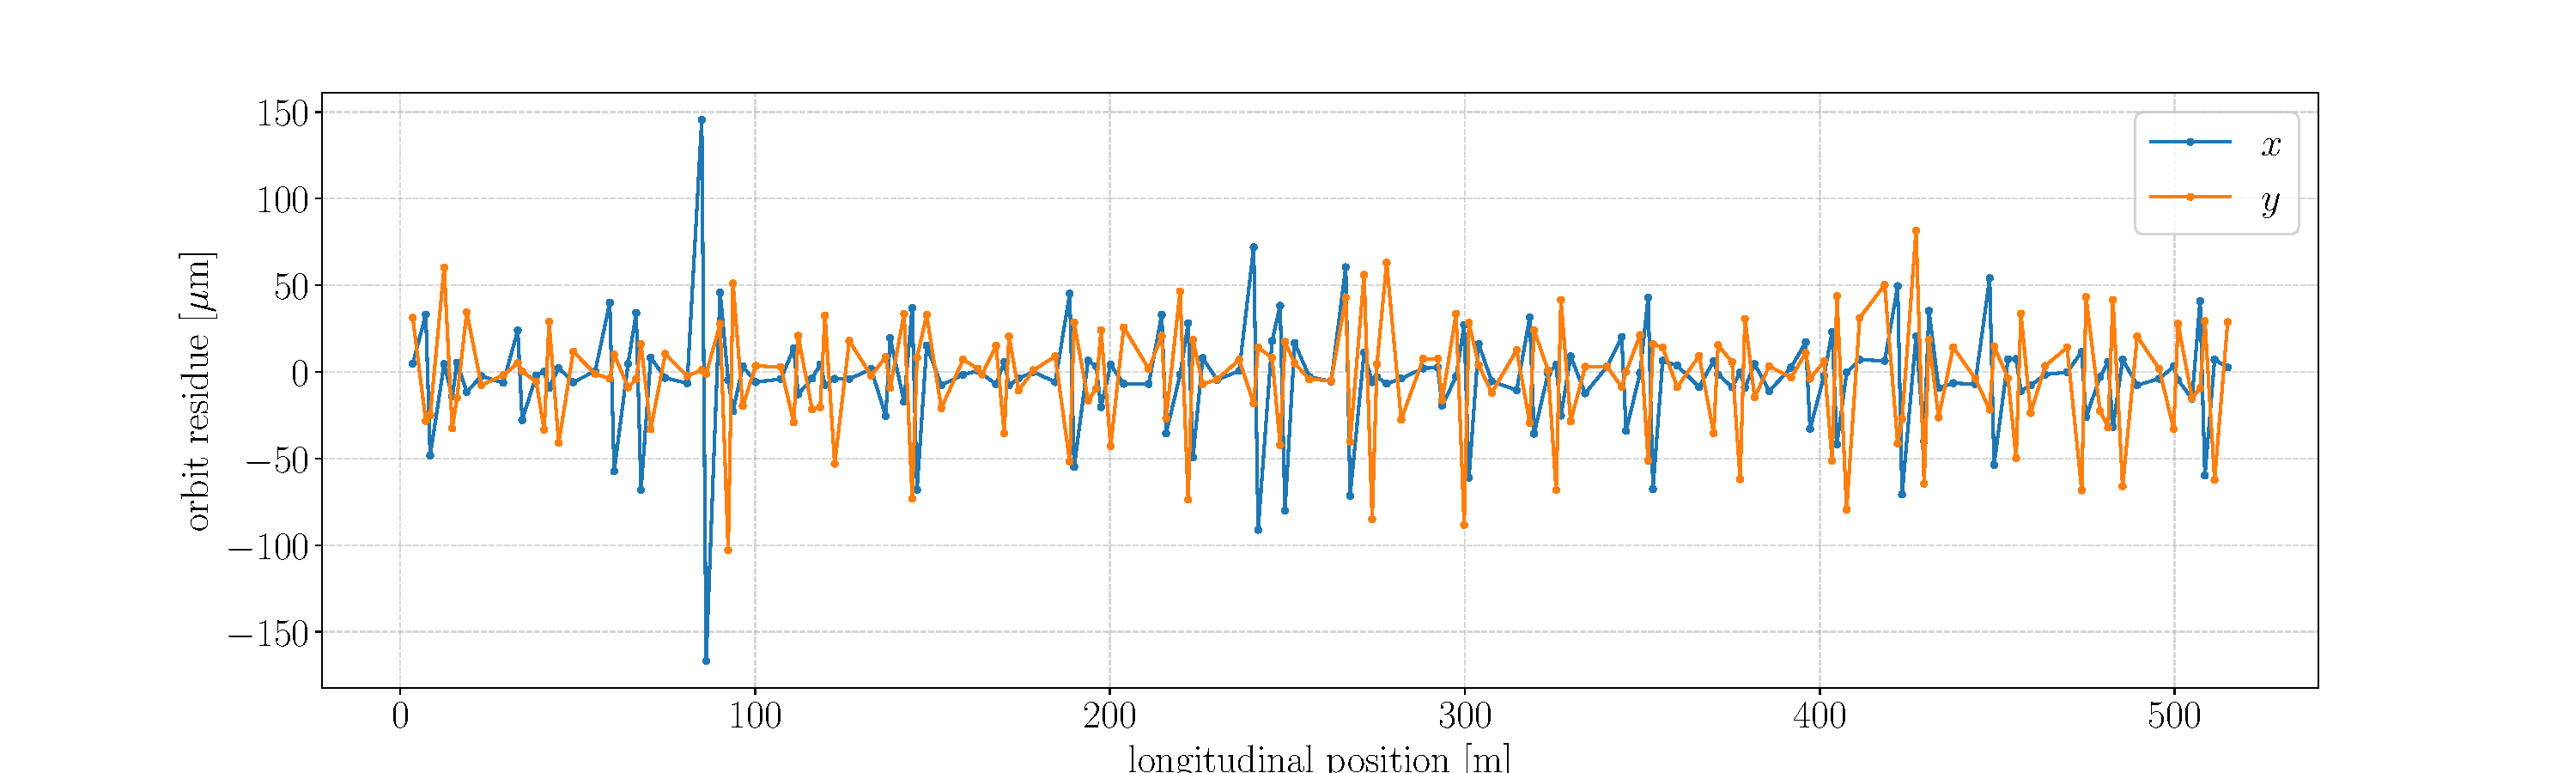
\includegraphics[width=1.0\textwidth]{figures/orbit_residue.pdf}
\caption{Residual orbit in Sirius storage ring.}
\label{fig:orbit_residue}
\end{figure}

The std values for the distortions in Figure~\ref{fig:orbit_residue} are $\SI{31}{\micro\meter}$ in horizontal plane and $\SI{32}{\micro\meter}$ in vertical. The peak-to-valley values are $\SI{312}{\micro\meter}$ and $\SI{184}{\micro\meter}$ for $x$ and $y$, respectively. From simulations, with alignment and field errors (within specified tolerances) on storage ring model, the orbit correction performance is better than the obtained in the actual ring. This is a strong indicative that the real alignment errors are greater than the specifications.

It is well-known that the magnetic fields in a storage ring depend on the relative transverse position deviations of the beam with respect to the magnets centers. This is the feed-down effect that was already mentioned throughout this work and is discussed in Appendix~\ref{appendix:feed-down}. Since very strong quadrupoles and sextupoles are used in Sirius~\gls{mba} lattice, it is expected that the dependencies of linear optics and coupling related to orbit distortions might play an important role.

To study the contribution of orbit distortion on optics and coupling, the residual orbit in the storage ring was reproduced in the nominal model. At this stage the betatron tunes were $\nu_x = 48.917$ and $\nu_y = 13.961$, and the tune were corrected to the nominal values. Notice that the distorted orbit produced large tune shifts of $\Delta \nu_x = -0.18$ and $\Delta \nu_y = -0.19$. An~\gls{orm} was calculated with this model and was used as input for a LOCO fitting with the same configuration used for the fitting of measured \gls{orm}s. Using the same kicks used for~\gls{orm} measurement, the initial difference between this~\gls{orm} and the nominal was $\chi = \SI{8.7}{\micro\meter}$. After the fitting, the final difference was $\chi = \SI{744}{\nano\meter}$. Observe that no noise was included in the goal~\gls{orm} and even so the minimum $\chi$ obtained after convergence was $\SI{676}{\nano\meter}$. Considering the measured Sirius BPM accuracy of $\SI{250}{\nano\meter}$ approximately, a rough estimate of this noise effect on data would increase the final $\chi$ close to the $\SI{1}{\micro\meter}$ level, which is the same level obtained in LOCO fittings from measured~\gls{orm} in the storage ring.

The qualitative behavior of LOCO fitting in this test was very similar to the fittings performed with measured~\gls{orm}. The~\gls{orm} could be adjusted in a very good level, both in on-diagonal and off-diagonal blocks. It was necessary to include the dispersion function in the fitting with weight $2$, otherwise the horizontal dispersion obtained with calibrated model did not match the dispersion from the perturbed orbit model. The vertical dispersion function could not be reproduced with LOCO model as well. 

Although there were no errors in BPM gains and roll angles and correctors gains, during the fitting these parameters were changed to adjust the~\gls{orm}. The results for these fit parameters are shown in Figure~\ref{fig:gain_fit_orb}.
\begin{figure}
\centering
\begin{subfigure}[t]{0.49\textwidth}
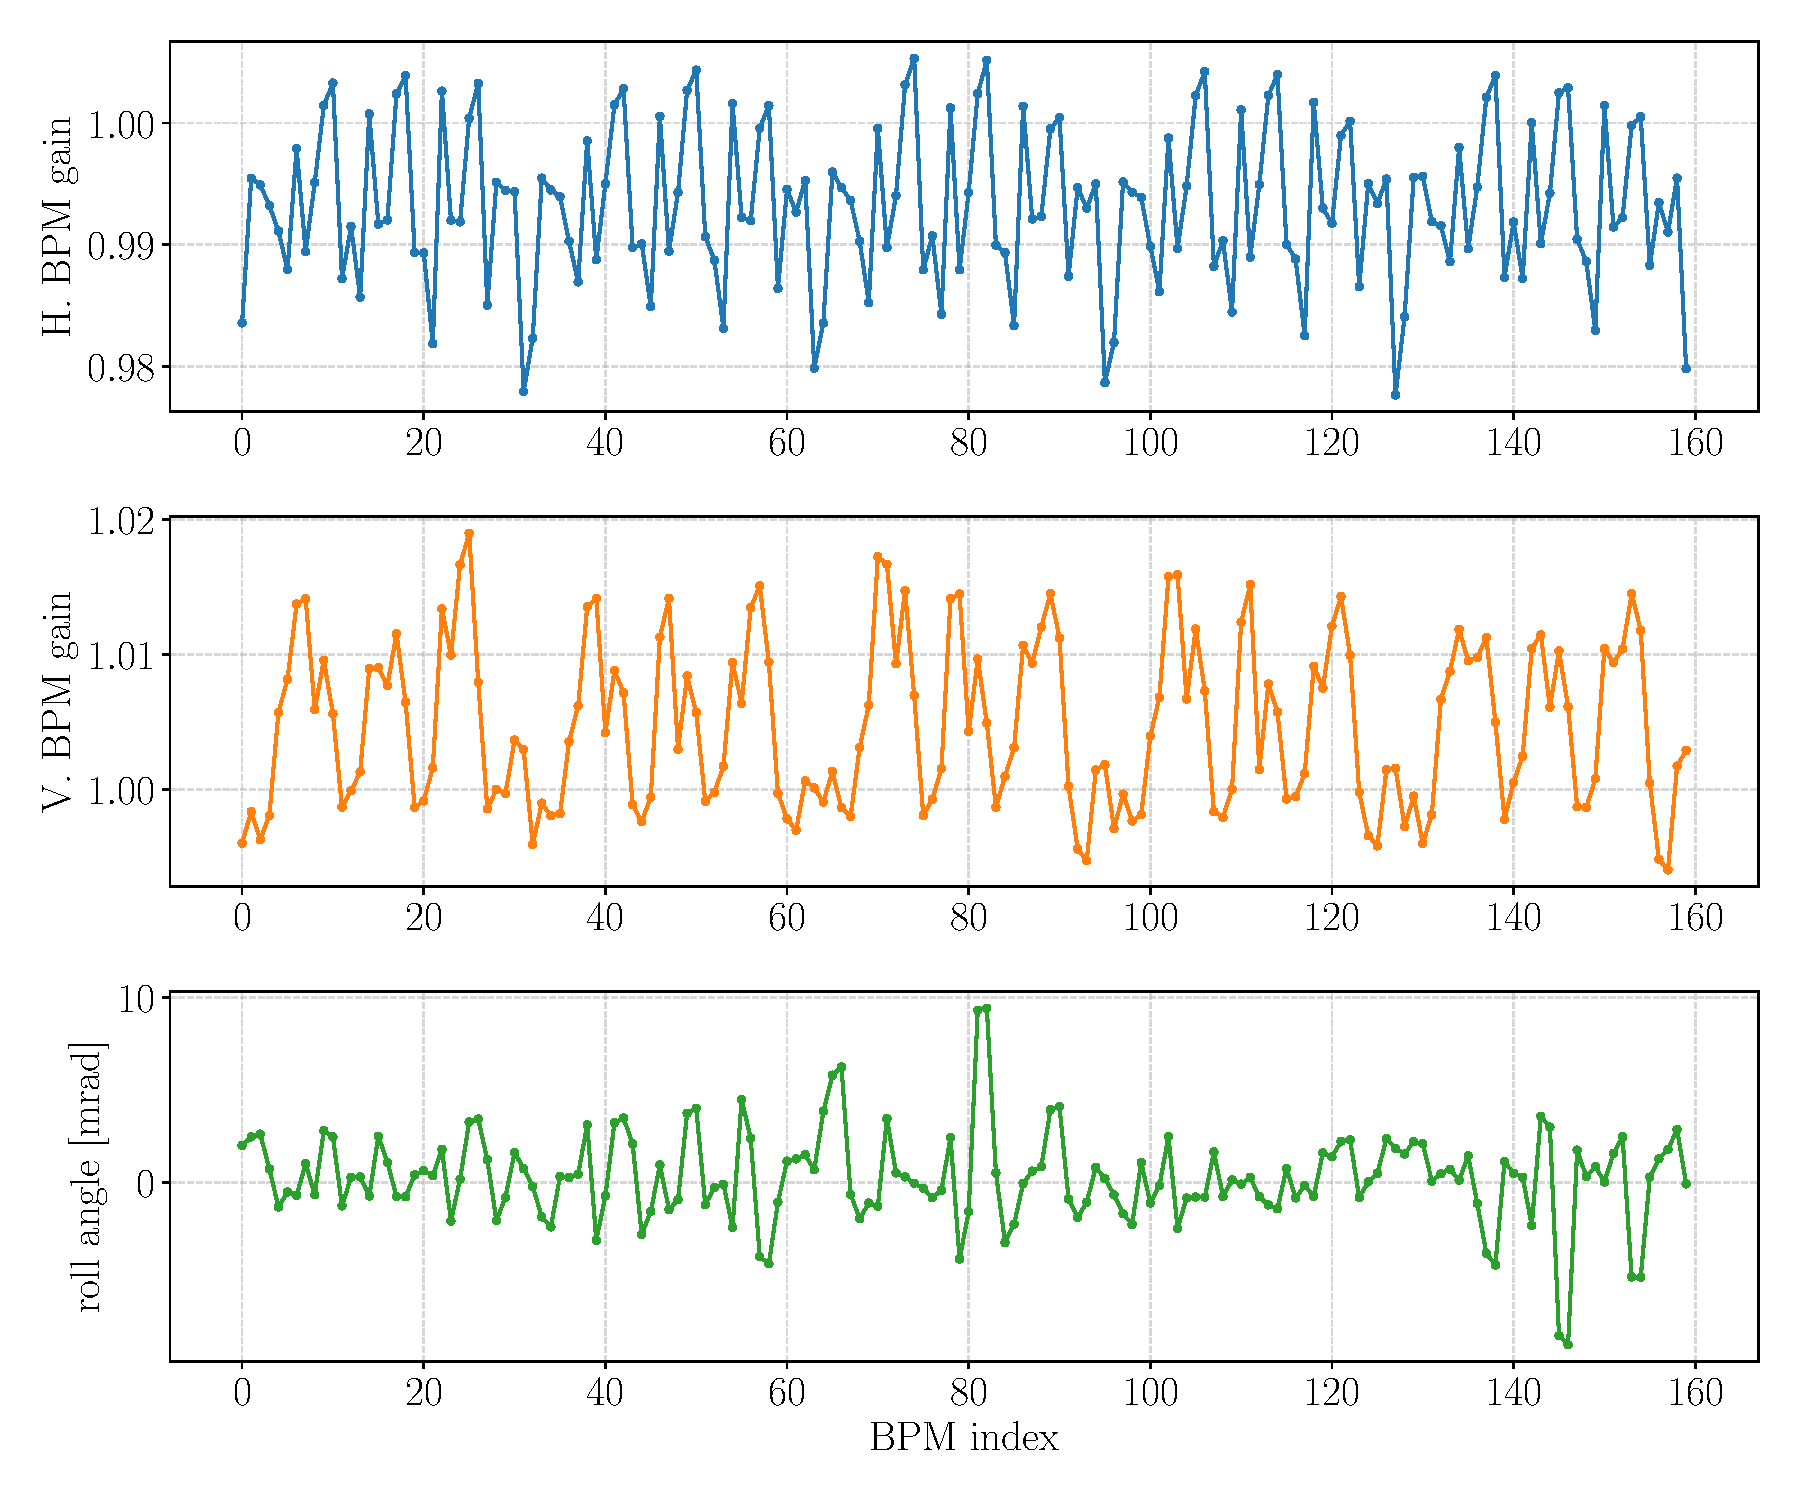
\includegraphics[width=1.0\textwidth]{figures/bpm_gains_orbit_distortion.pdf}
    \caption{BPM gains and roll angles.}
    \label{subfig:bpm_fit_orb}
\end{subfigure}
 \begin{subfigure}[t]{0.49\textwidth}
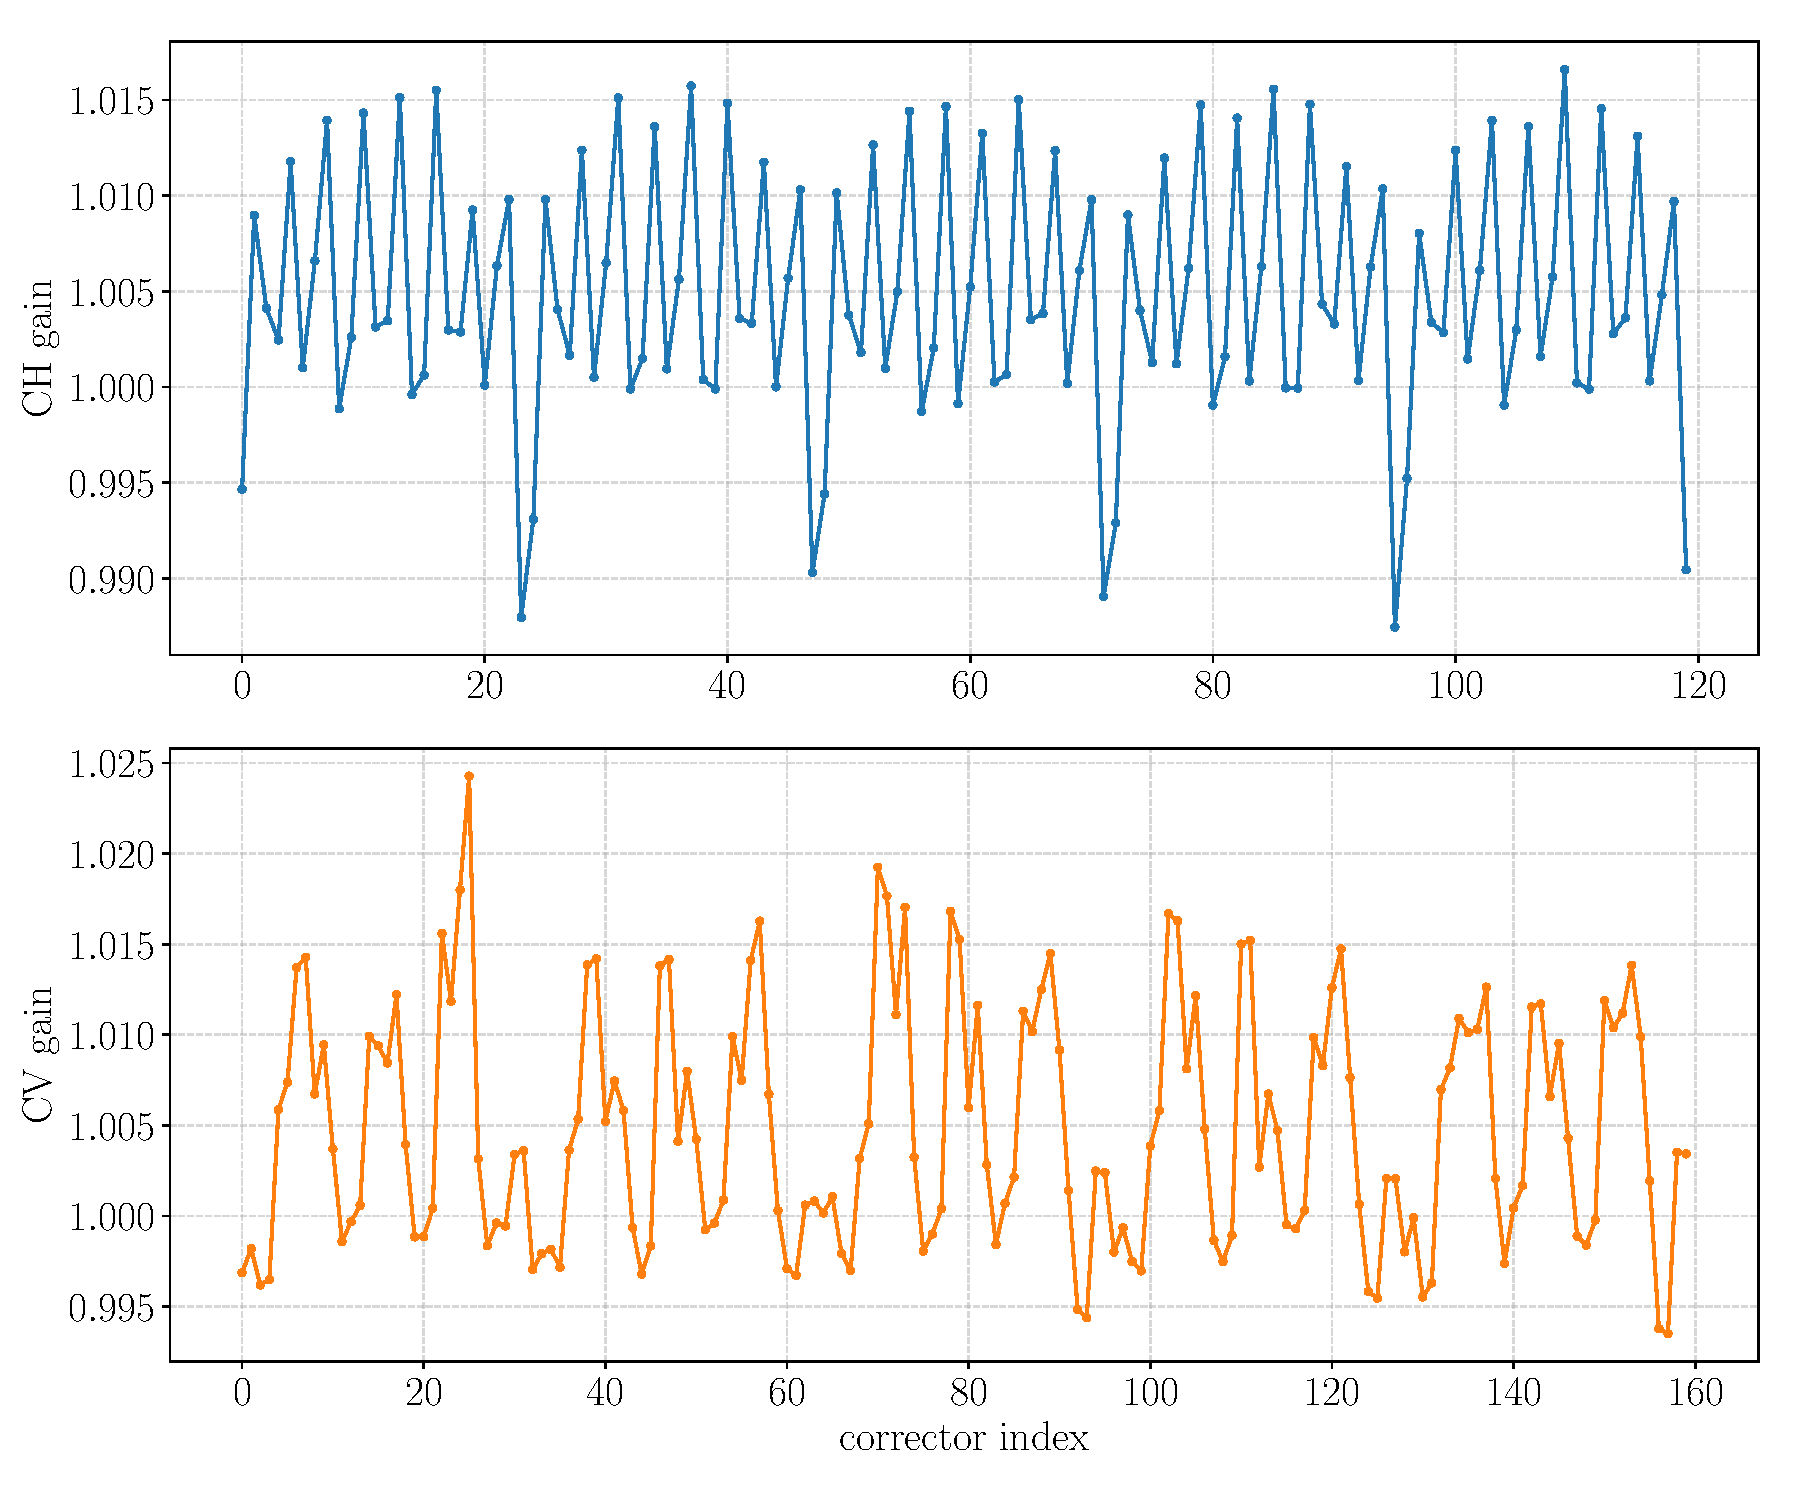
\includegraphics[width=1.0\textwidth]{figures/corr_gains_orbit_distortion.pdf}
    \caption{Correctors gains.}
    \label{subfig:corr_fit_orb}
\end{subfigure}
\caption{Fitted values for BPM gains, roll errors and correctors (CH and CV) gains for model with perturbed orbit.}
\label{fig:gain_fit_orb}
\end{figure}

Observe that there is also a periodic signature in the gains. Comparing with Figure~\ref{fig:gain_fit}, even tough the absolute values are smaller than the gains obtained in the previous fitting, the periodic signature observed previously (specially for correctors) can be related to the orbit distortion effect on gains fitting. The BPM roll angles adjusted in this test were also on the order of $\pm\SI{10}{\milli\radian}$. Thus the values obtained previously probably are unrealistic and also related to the orbit contribution.

The beta-beating caused by the residual orbit were also calculated and compared with the first calibrated LOCO model. The results are presented in Figure~\ref{fig:beta_beating_orb}. The disturbed orbit produced~\gls{std} beta-beatings of $\SI{8.6}{\%}$ in horizontal and $\SI{3.0}{\%}$ in vertical plane. It can be seen that the orbit contributions to the beta-beating in some locations are commensurable to the ones obtained from calibrated model. The fact that calibrated beta-beating is higher than the cause by orbit distortion is reasonable, since in the real storage ring there are other sources of optics perturbations. 
\begin{figure}[h!]
\centering
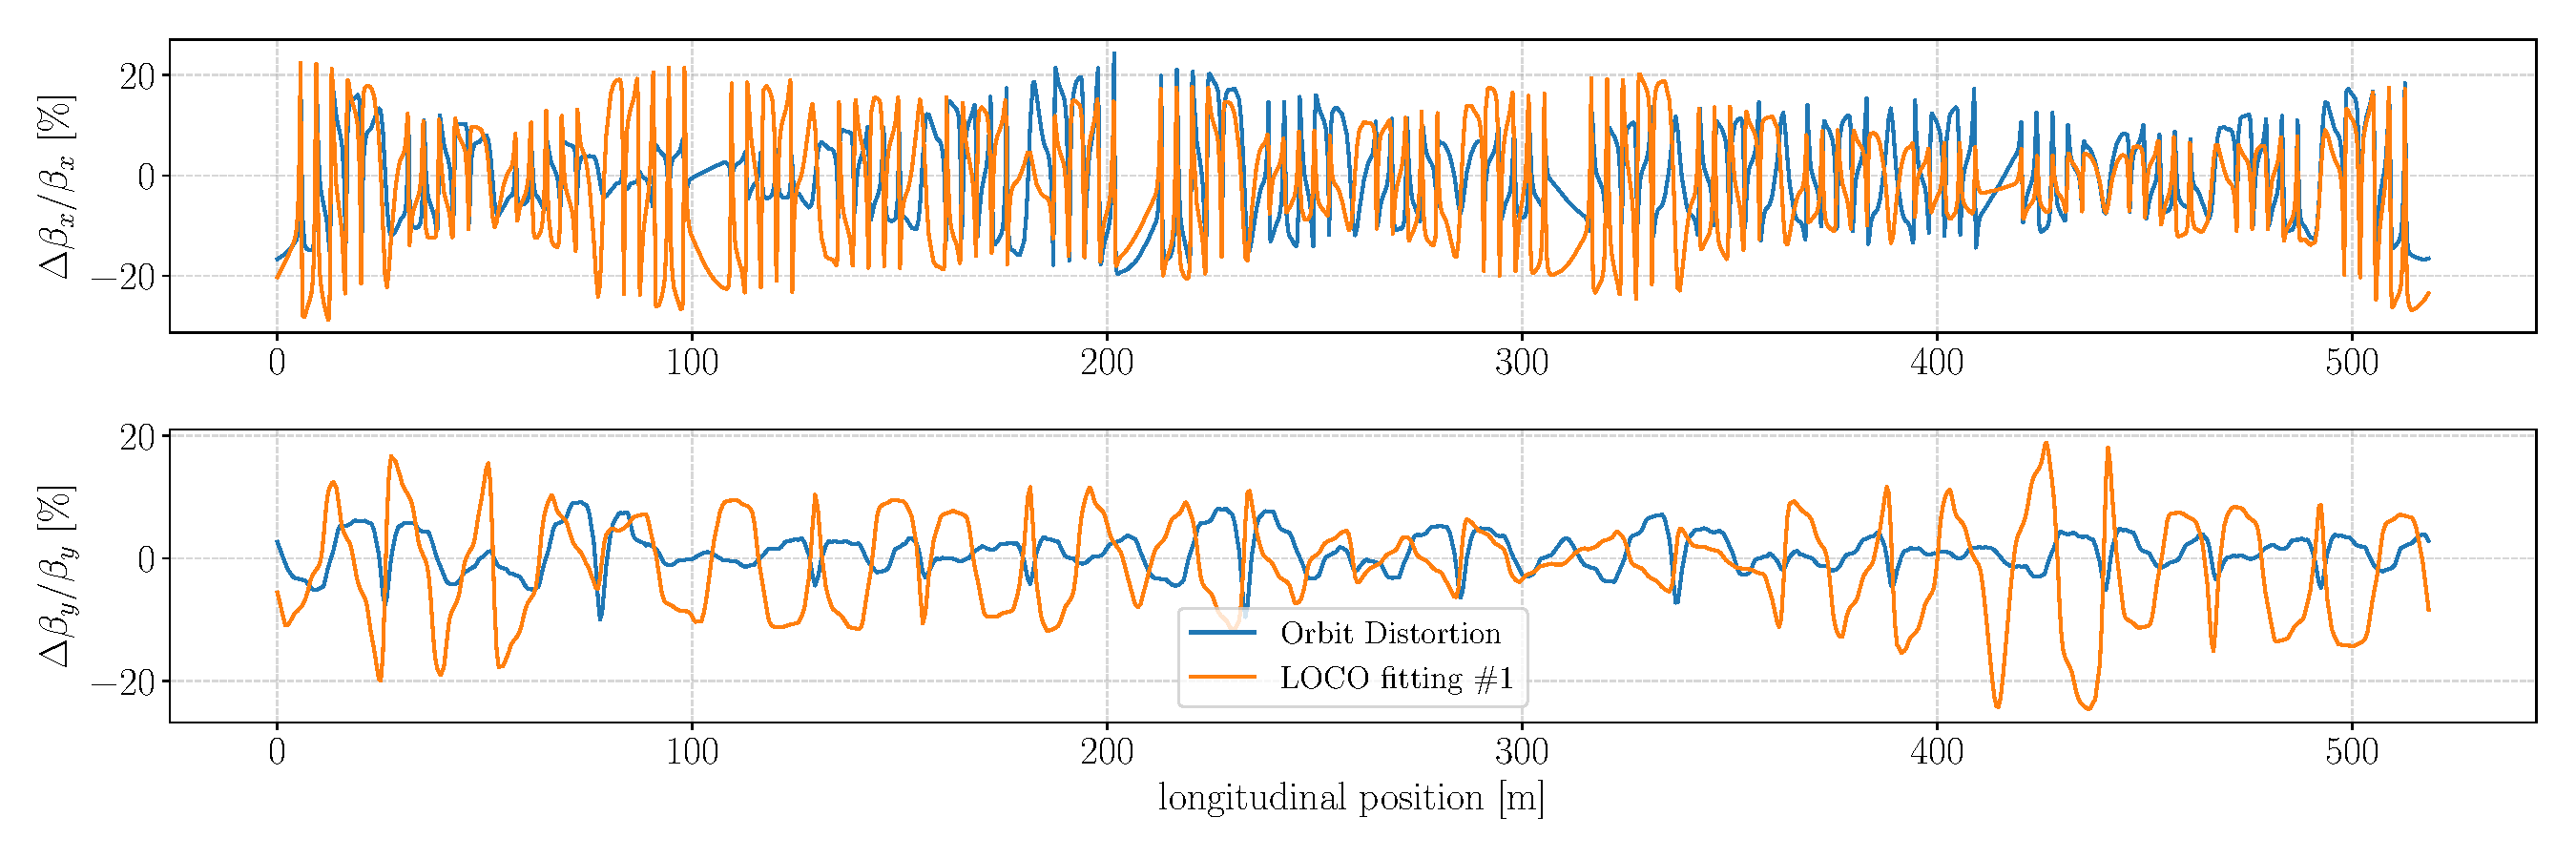
\includegraphics[width=1.0\textwidth]{figures/beta_beating_orbit_loco_iter0.pdf}
\caption{Beta-beating comparison from perturbed orbit model with first LOCO calibrated model.}
\label{fig:beta_beating_orb}
\end{figure}

Another comparison was performed between the dispersion functions from perturbed orbit model and the measurements realized on storage ring before LOCO corrections, plotted in Figure~\ref{fig:disperson_orb}. Once again, the actual errors are larger than the ones generated by feed-down effect, as expected. The vertical dispersion signature similarities draws attention. It is clear that the errors in $\eta_y$ caused by orbit distortion explain a great part of the measured $\eta_y$. The correlation between measured $\Delta\eta_x$ and the calculated with orbit distortions is $76\%$ and for $\Delta\eta_y$ the correlations is $53\%$. The main sources of $\eta_y$ are vertical dipolar fields created by vertical orbit distortions at quadrupoles.
\begin{figure}[h!]
\centering
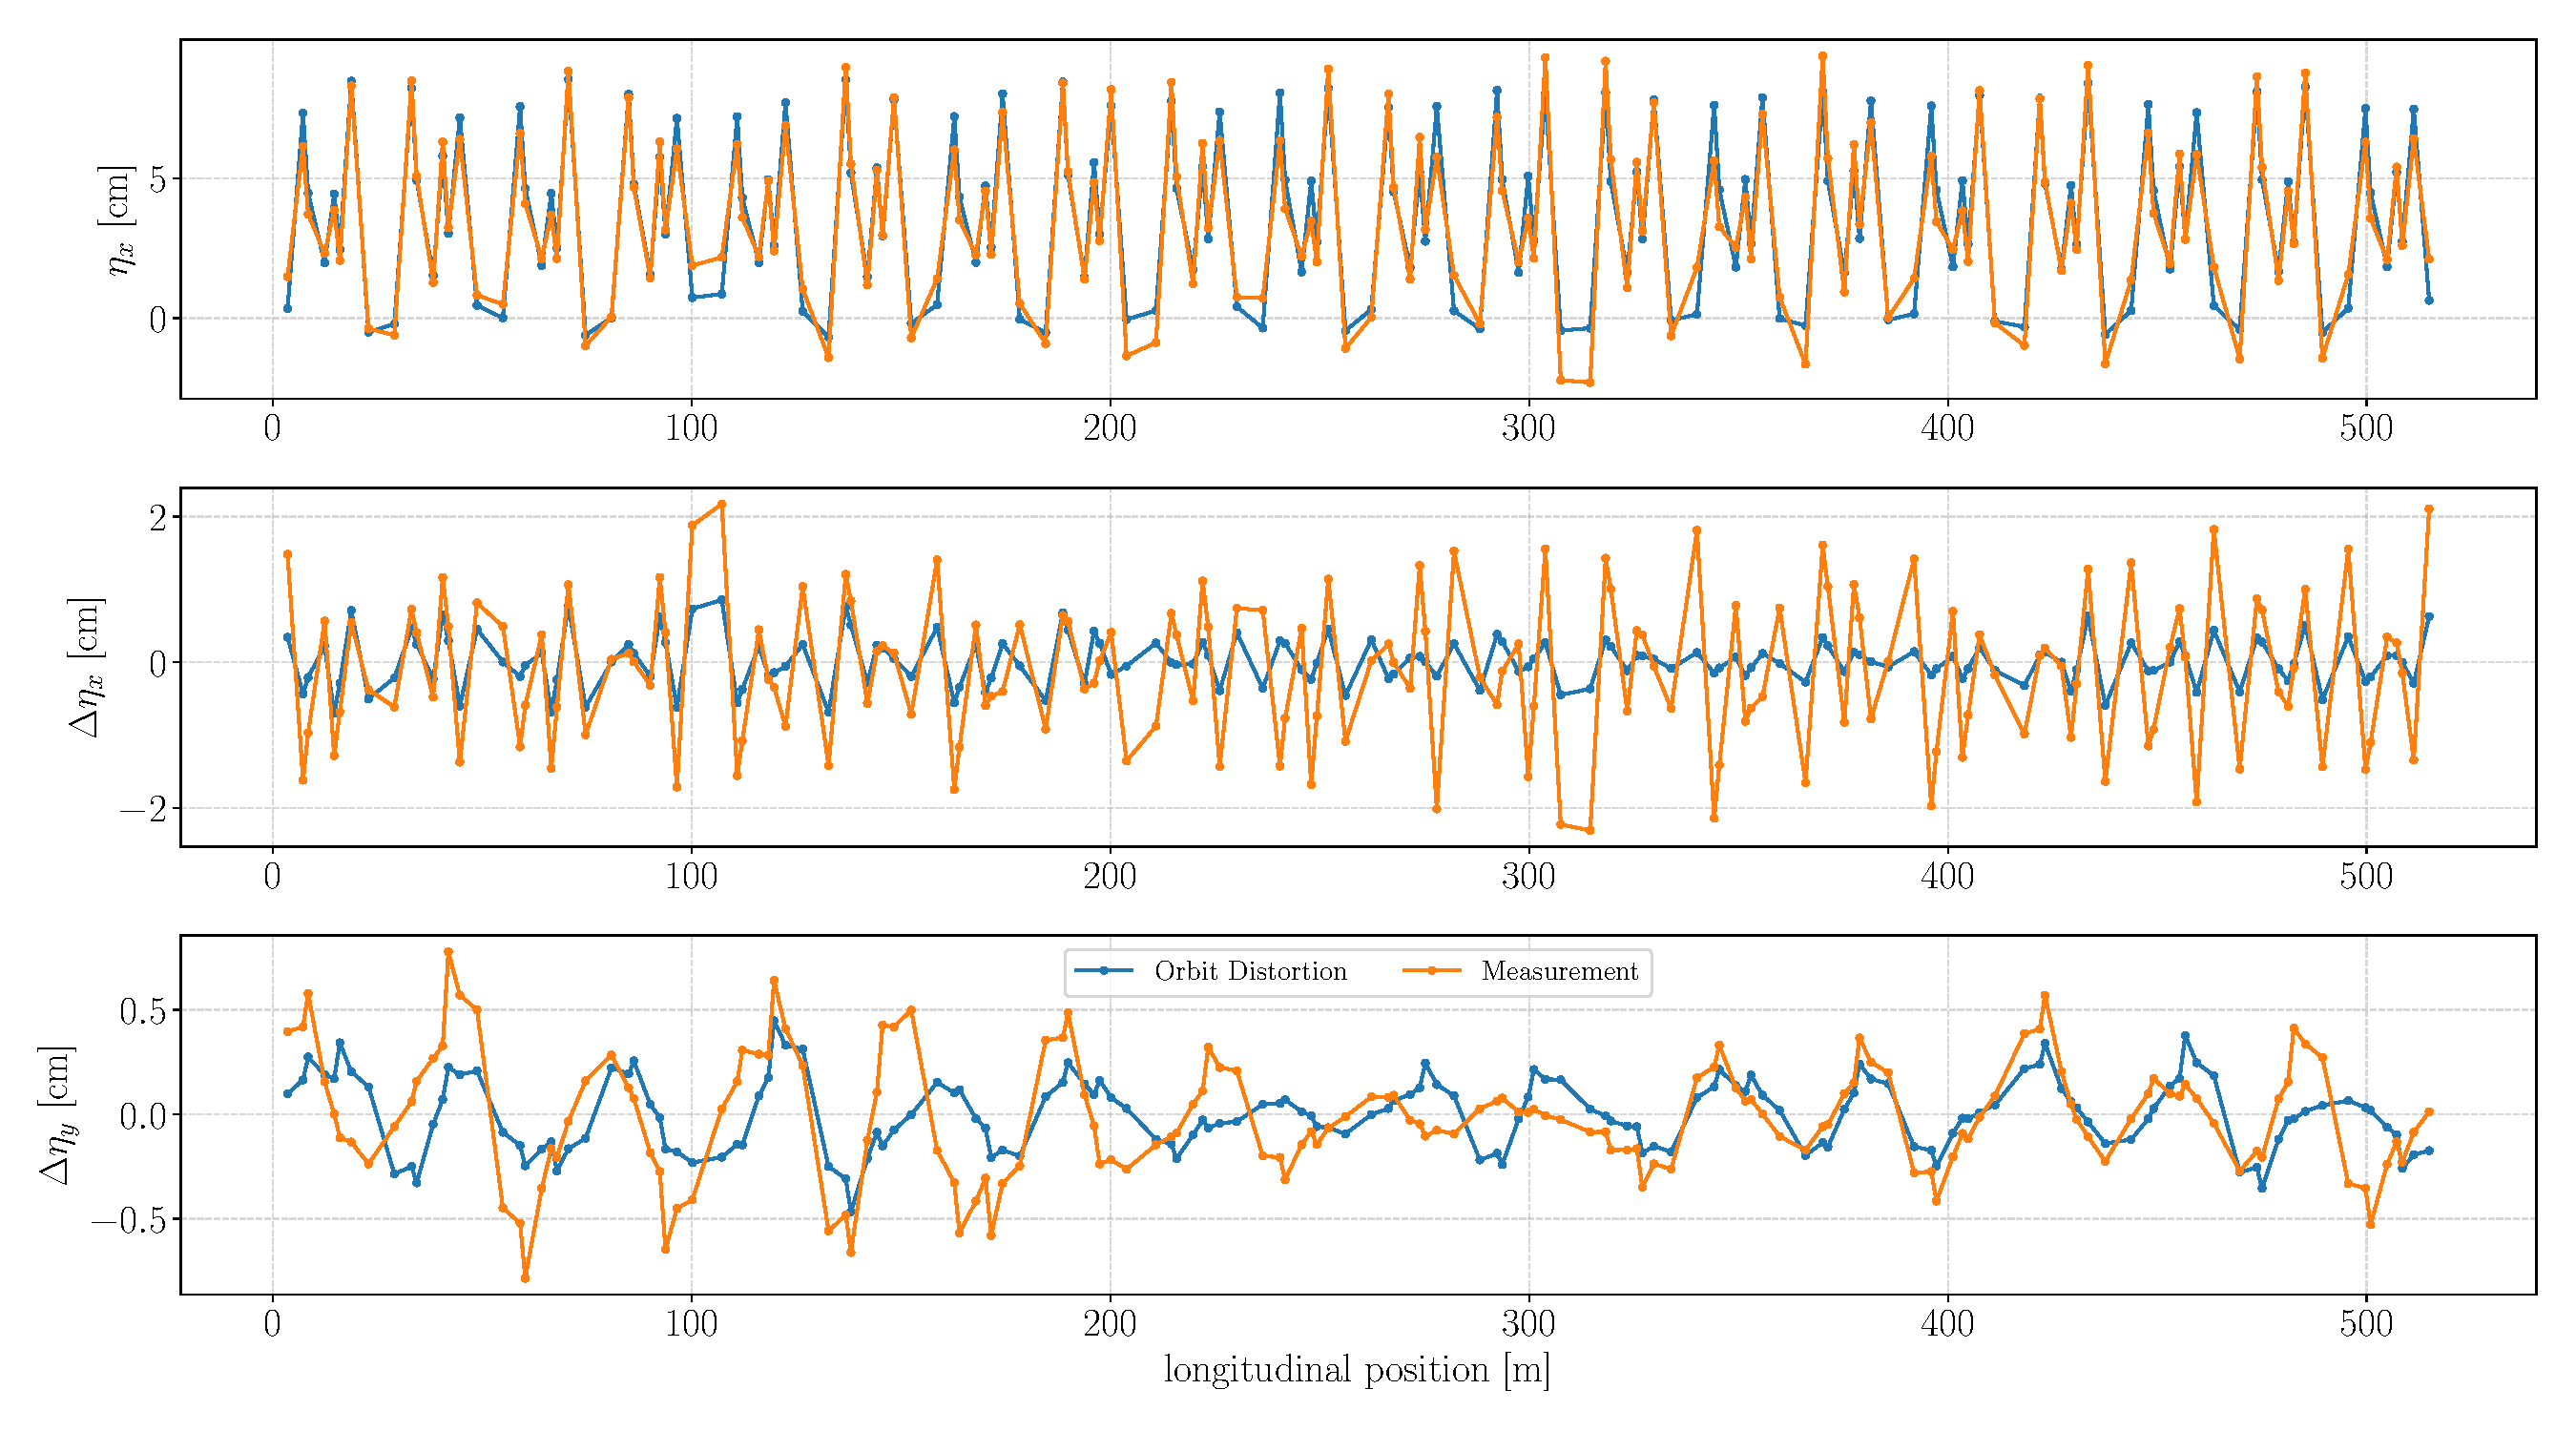
\includegraphics[width=1.0\textwidth]{figures/dispersion_orbit_iter0.pdf}
\caption{Comparison dispersion functions at BPMs obtained perturbed orbit model with measurement before optics corrections.}
\label{fig:disperson_orb}
\end{figure}

Finally, the variations in normal and skew quadrupoles obtained in this test were compared with LOCO corrections applied in storage ring, as can be seen in Figure~\ref{fig:corrections_orb}.
\begin{figure}[h!]
\centering
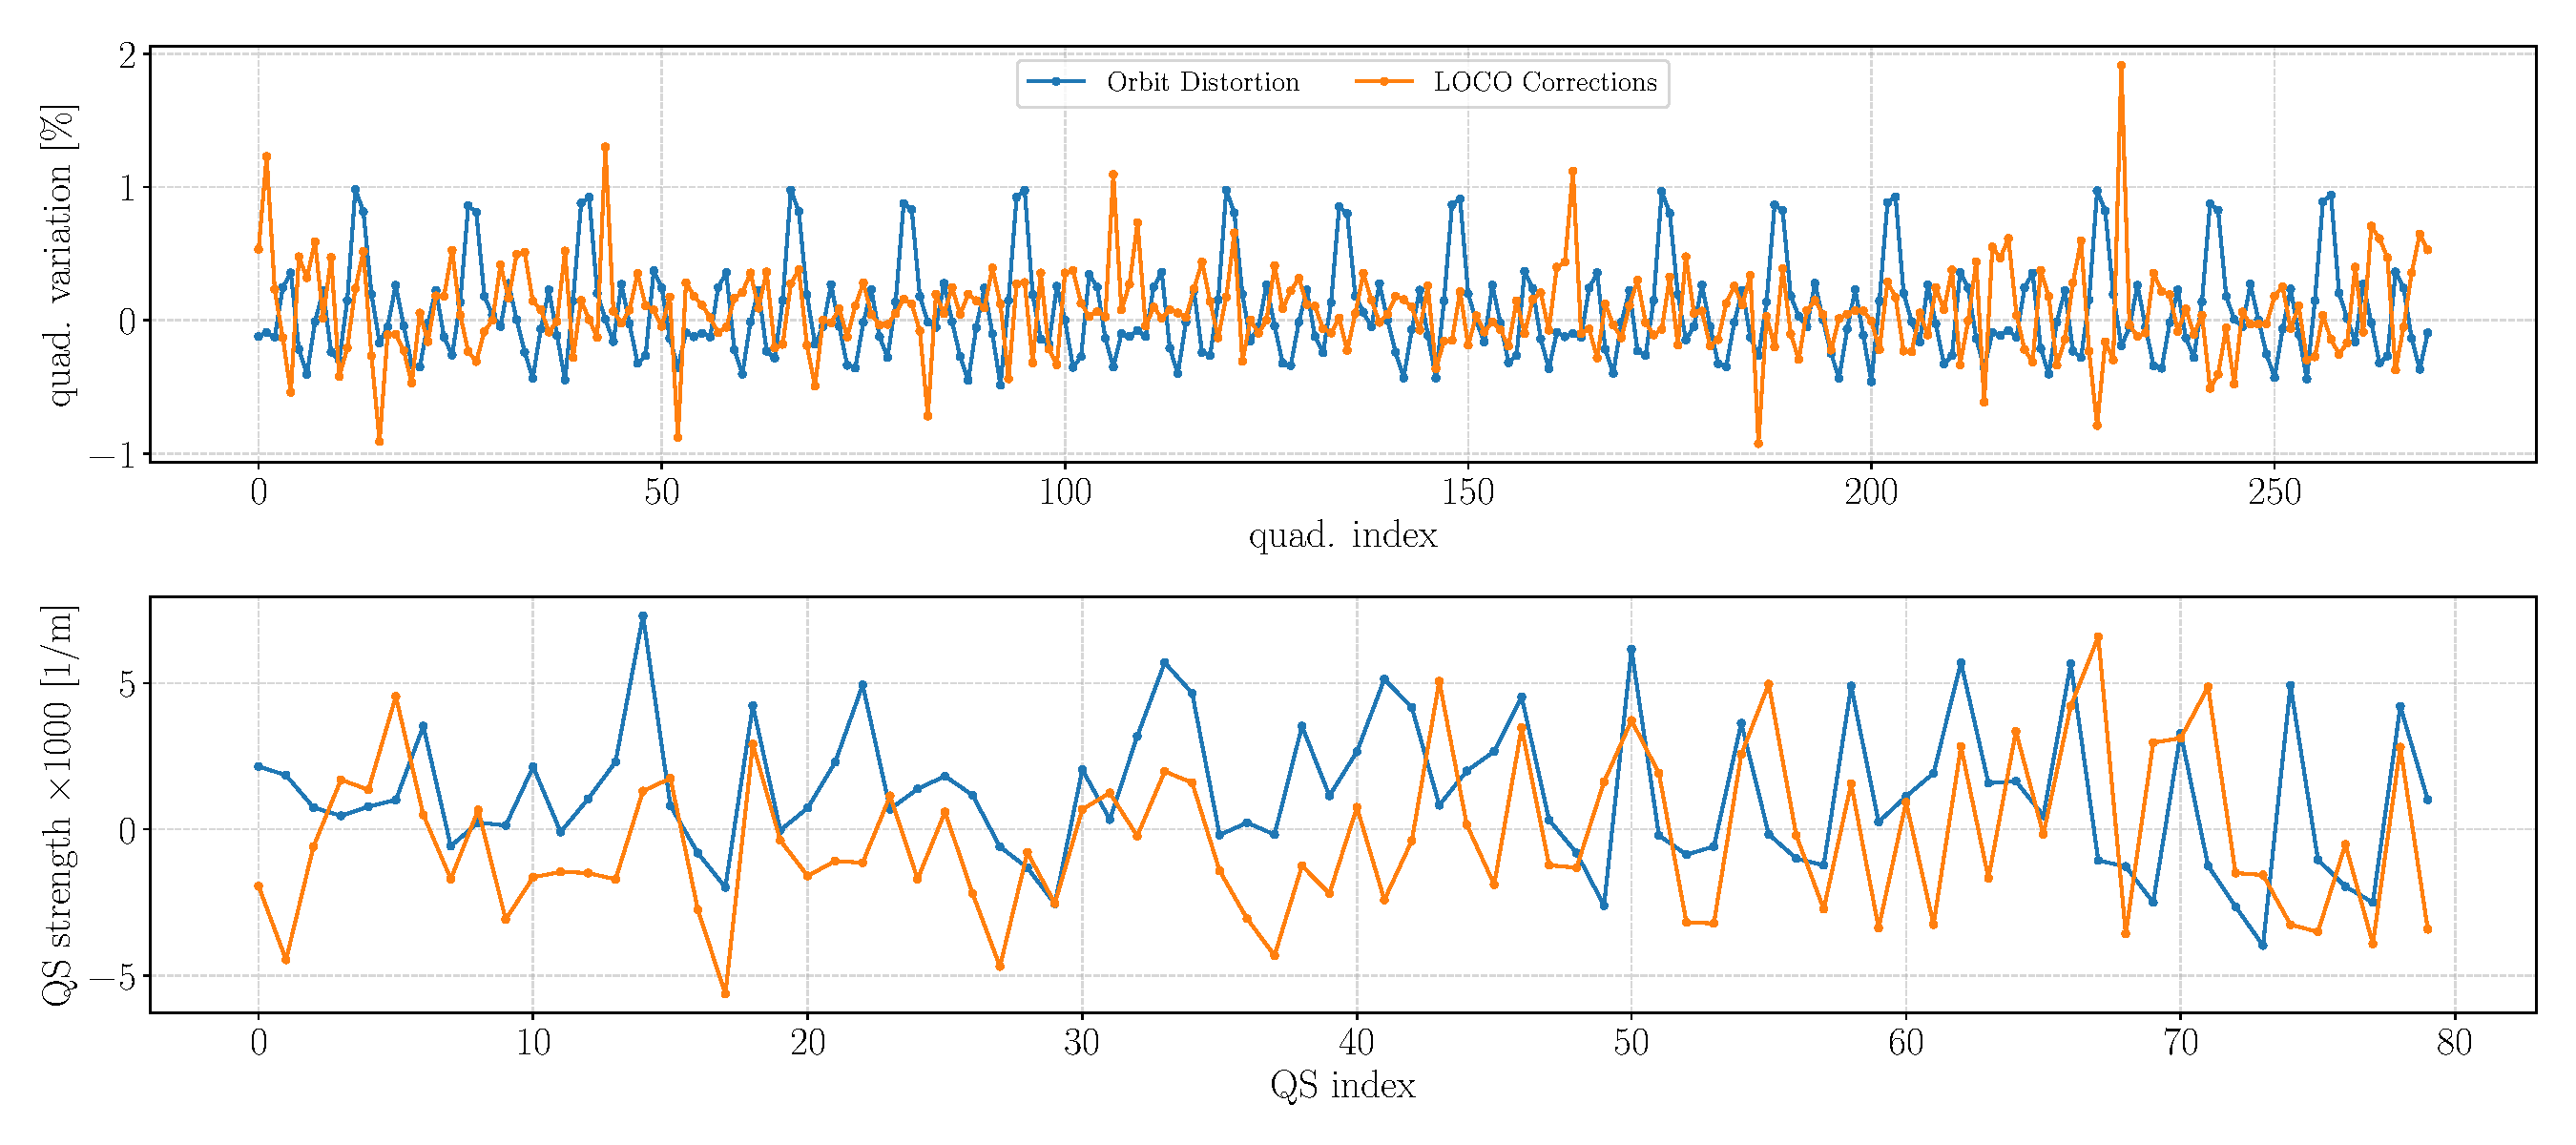
\includegraphics[width=1.0\textwidth]{figures/corrections_orb_residue_loco_iter0.pdf}
\caption{Normal and skew quadrupoles variation for perturbed orbit model and the first LOCO calibrated model.}
\label{fig:corrections_orb}
\end{figure}

The order of magnitude of variations in both cases are very similiar. For quadrupoles, the std variations are $\SI{0.36}{\%}$ for orbit perturbed model and $\SI{0.33}{\%}$ for LOCO corrections. For skew quadrupoles, the std variations are $\SI{2.4e-3}{\meter^{-1}}$ for orbit perturbed model and $\SI{2.7e-3}{\meter^{-1}}$ for LOCO corrections. When these corrections are applied in the perturbed model, the~\gls{orm} is approximated to the nominal matrix very well, the optics errors are reduced (except for $\eta_y$) but can not be eliminated, exactly as observed in the actual storage ring. The results of optics corrections on perturbed model is organized on Table~\ref{tab:params_corr}.
\begin{table}[h!]
    \centering
    \caption{Optics errors before and after LOCO corrections applied on perturbed model.}
    \label{tab:params_corr}
    \begin{tabular}{cccc}
        \toprule\toprule
        Parameter (std) & before corr. & after corr. & Unit\\
        \hline
        $\Delta\beta_x/\beta_x$ & \SI{8.6}{} & \SI{1.8}{} & \SI{}{\%}\\
        $\Delta\beta_y/\beta_y$ & \SI{3.0}{} & \SI{1.5}{} & \SI{}{\%}\\
        $\Delta\eta_x$ & \SI{3.3}{} & \SI{1.6}{} & \SI{}{\milli\meter} \\
        $\Delta\eta_y$ & \SI{1.7}{} & \SI{1.9}{} & \SI{}{\milli\meter}\\    
        \bottomrule\bottomrule
    \end{tabular}
\end{table}

% From this tests its is clear that the orbit plays an important role on Sirius storage ring optics. When the residual orbit measured on the actual ring is reproduced in the model, the behavior of LOCO fitting with measured data was also observed in the fitting of~\gls{orm} generated with the disturbed orbit. More than that, the magnitudes and signatures of betatron and dispersion function disturbances

From this results it can be seen that even with nominal gradients on lattice, the linear optics perturbations generated by orbit distortions could be reduced but there is a limitation for this scheme of correction. The off-diagonal elements in ORM can be greatly reduced with skew quadrupoles, however since the vertical dispersion function could not be adjusted with LOCO fitting, it could not be correct as well (in fact, the error was even increased). 

The qualitative behavior of LOCO analysis using an ORM calculated from a model with the same residual orbit as measured in Sirius storage ring reproduces the behavior that is observed with measured ORM. Since in the real machine there are other errors that also perturbs the linear optics, it is expected that the minimum level of optics correction with a disturbed orbit is higher than the level obtained in this test. 

This test provides an explanation for the incapacity of LOCO fitting to predict accurately the storage ring optics. LOCO, as included in the method name, is a process to obtain the linear optics. However, it can be concluded that non-linear effects are perturbing the Sirius optics, caused by orbit distortions. The origin for this residual orbit is the magnets misalignment in storage ring, which was already confirmed with measurements performed by LNLS Alignment Group. Another explanation for these problems might be the incompatibility between the storage ring model and the actual storage ring regarding the elements longitudinal positions, i.e., the model would not accurately describe the storage ring. 

The betatron function depends basically on the focusing strengths introduced by quadrupoles, while the dispersion function depends both on focusing and deflecting forces. Orbit distortions in quadrupoles introduce additional dipolar fields and in sextupoles extra gradients are introduced by the feed-down effect. With the LOCO fitting, only the quadrupoles are varied to fit the linear optics. So if the quadrupoles are used to compensate the gradients in sextupoles to fix the betatron function, the additional dipolar fields in quadrupole will also be changed, perturbing the dispersion function. On the other hand, if the quadrupoles are used to compensate the dipolar fields in quadrupoles and fix the dispersion function, the gradients in sextupoles are changed and the betatron functions are perturbed. Therefore, in the presence of large orbit distortions, it is only possible to balance the correction of betatron function without perturbing the dispersion (or vice-versa), reaching a limited level of correction effectiveness.

Furthermore, this type of correction that uses quadrupoles to compensate perturbations generated by orbit distortion are really inadequate. The actual solution is to mitigate the alignment problems that limit the residual orbit, so the orbit can be best corrected to the magnetic centers, reducing its effect on linear optics. After that, it is expected that the major contributions to the optics perturbations come mainly from gradient errors from fields discrepancies of quadrupoles. Hence, the LOCO corrections should fix these deviations and the optics errors should be corrected to a better level. A realignment campaign in Sirius is scheduled for January, 2021. In this campaign the devices longitudinal positions will also be measured and will be used to improve the storage ring model. After that, the machine will be re-commissioned and it is expected that LOCO analysis can be performed again to obtain a better level of correction for storage linear optics.
